\documentclass[oneside,letterpaper,12pt]{book}
\usepackage[margin=1in,letterpaper]{geometry}  
% http://graduateschool.usc.edu/wp-content/themes/fictional-university-theme/assets/doc/Manuscript_Formatting_and_Documentation_Styles.pdf
% Paper: 8.5" x 11" -- letter paper
% Margins:
%    All margins 1" 
%    Footer margin, page number must be 0.5" from the bottom
%    Except page number, everything else must fit within margin
% Spacing:
%    Double space text throughout manuscript and indent paragraphs
%    Sing space footnotes, long quoted para, fig and tab captions, items in lists and tables
%    Bibliography (if style manual requires ) single space within entry, and double space between entries  
% Font style and size:
%    be consistent
%    regular para text: 11 or 12 pt
%    chapter title and main section heading, at least 16pt
%    footnote, caption, eqns, within figs & tabs: atleast 9pt
%    Color: black, except for hyerplinks, within tabs and figs
%    bold for headings, chapter, section, sub section etc
% Page num:
%    0.5" from bottom; either center or right but be consistent
%    dont bold or italicize
%    same font family as body text
%    
% [[ Pagination and order see PDF in the above link]]  
%    

\usepackage{sectsty}
%\chapternumberfont{\Large} 
%\chaptertitlefont{\LARGE}
\chapternumberfont{\fontsize{20pt}{20pt}\selectfont} 
\chaptertitlefont{\fontsize{20pt}{20pt}\selectfont}


\usepackage[T1]{fontenc}
\usepackage[tt=false, type1=true]{libertine} 
\usepackage[varqu]{zi4}
\usepackage{amsfonts}
\usepackage{amsmath}
\usepackage{amssymb}
\usepackage[libertine]{newtxmath}


% Packages required by `USCthesis.sty`.
\usepackage{setspace}
\usepackage{tabularx}
%\usepackage{biblatex}

% Filler text for formatting. Comment these lines out for real writing.
% \usepackage[english]{babel}
% \usepackage{blindtext}

%\usepackage{times}
\usepackage{microtype}
% \usepackage{latexsym}


\usepackage{hyperref}
\usepackage{xcolor}		% make links dark blue
\definecolor{darkblue}{rgb}{0, 0, 0.5}
\hypersetup{colorlinks=true,citecolor=black, linkcolor=black, urlcolor=darkblue}
\hypersetup{colorlinks=true, citecolor=darkblue, linkcolor=black, urlcolor=darkblue}
  

\usepackage{makecell}
\usepackage{lscape} 
\usepackage{subcaption}
\usepackage{latexsym}
\usepackage{multirow}
\usepackage{rotating}
\usepackage{comment}
\usepackage{arydshln}
\usepackage{float}
\usepackage{subcaption}
\usepackage{enumitem}
\usepackage{xspace}
%\usepackage{textgreek}
\usepackage{booktabs}
\usepackage{tocbibind}
\usepackage{epigraph} 


\DeclareMathOperator*{\argmax}{arg\,max}
\DeclareMathOperator*{\argmin}{arg\,min}
\usepackage{mathtools}
\DeclarePairedDelimiter\abs{\lvert}{\rvert}

\usepackage{color}
\usepackage[finalizecache,cachedir=minted-cache]{minted} 
\usepackage{tikz}
\usepackage[normalem]{ulem}

\usetikzlibrary{positioning,fit,calc,backgrounds}
\tikzset{block/.style={draw,thick,text width=2cm,minimum height=1cm,align=center},
         line/.style={-latex}
}
\makeatletter
\def\ruwave{\bgroup \markoverwith{\lower3.5\p@\hbox{\textcolor{red}{\sixly \char58}}}\ULon}
\font\sixly=lasy6
\makeatother


% Weiqiu
\usepackage{wasysym}
\usepackage{etoolbox}
\usepackage{siunitx}
\robustify\bfseries
\sisetup{
 table-number-alignment=right,
 table-text-alignment=right,
 detect-weight,
 detect-shape,
 mode=math,
 math-rm=\mathtt
}
% \usepackage{enumitem}
\newcommand{\subscript}[2]{$#1 _ #2$}

\usepackage{natbib}
%\usepackage[nottoc,numbib]{tocbibind}
\renewcommand\cite{\citep}	% to get "(Author Year)" with natbib    
%\newcommand\shortcite{\citeyearpar} % to get "(Year)" with natbib    
\newcommand\newcite{\citet}	 % to get "Author (Year)" with natbib   


\usepackage{graphicx}
\graphicspath{{img/}{img/optimvocab/}}


\newlength\myheight
\newlength\mydepth
\settototalheight\myheight{Xygp}
\settodepth\mydepth{Xygp}
\setlength\fboxsep{0pt}
\newcommand*\inlinegraphics[1]{%
  \settototalheight\myheight{Xygp}%
  \settodepth\mydepth{Xygp}%
  \raisebox{-\mydepth}{\includegraphics[height=\myheight]{#1}}%
}


\newcommand\BibTeX{B\textsc{ib}\TeX}
\newcommand{\bleu}{{\textsc{Bleu}}}
\newcommand{\chr}[2]{{C\small{HR}{#1}$_{{#2}}$}}
\newcommand{\chrx}[1]{\text{\small{CHR}\large{#1}}}

\newcommand{\chrf}[1]{\textsc{ChrF}{$_{#1}$}}
\newcommand{\bleufx}[1]{{B\small{LEU}F$_{{#1}}$}}
\newcommand{\bleuf}{{\textsc{BleuF}}}

\newcommand{\maf}[1]{\textsc{MacroF}{\text{$_{{#1}}$}}}
\newcommand{\mif}[1]{\textsc{MicroF}{\text{$_{{#1}}$}}}
\newcommand{\mableu}{\textsc{MacroBleu}}
\newcommand{\mibleu}{\textsc{MicroBleu}}
\newcommand{\blrtmn}{\textsc{BLEURT}\text{\footnotesize{}mean}}
\newcommand{\blrtmd}{\textsc{BLEURT}\text{\footnotesize{}median}}

%\usepackage{amssymb}
\newcommand{\deleterious}[3]{{\Large\frownie{}}_{#1\to#2}^{#3}}
\newcommand{\beneficial}[3]{{\Large\smiley{}}_{#1\to#2}^{#3}}
\newcommand{\scoredel}[3]{\delta_{#3}^{#1^{#2}}}





\newcommand{\colorann}[3]{\textcolor{#1}{${}^{#2}[$#3$]$}}
\newcommand{\tg}[1]{\colorann{blue}{TG}{#1}}
%\newcommand{\colorann}[3]{\textcolor{#1}{${}^{#2}[$#3$]$}}
%\newcommand{\jon}[1]{\colorann{red}{Jon}{\footnotesize #1}}
%\newcommand{\tg}[1]{\colorann{cyan}{TG}{\footnotesize #1}}
%\newcommand{\wy}[1]{\colorann{orange}{WY}{\footnotesize #1}}
%\newcommand{\cl}[1]{\colorann{green}{CL}{\footnotesize #1}}

\newcommand{\insig}{$^{\times}$}



\newcommand{\mtdata}{\textsc{MTData}}
\newcommand{\nlcodec}{\textsc{NLCodec}}
\newcommand{\nldb}{\textsc{NLDb}}
\newcommand{\rtg}{\textsc{RTG}}

\newcommand{\sentpiece}{SentencePiece}
\newcommand{\sacrebleu}{\textsc{SacreBleu}}
\newcommand{\hftok}{HuggingfaceTokenizers}

  % all the imports and stuff
\pagestyle{plain}


\begin{document}

\begin{titlepage}
	\centering
	\vspace{1cm}
	{\large Dissertation Proposal \par}
	\vspace{2mm}
	{\large Submitted in partial fulfillment of \\ the requirements for the degree of }\\
	\vspace{1mm}
	{\scshape\large Doctor of Philosophy \\ \vspace{1mm} (Computer Science)}
	\vspace{1.5cm}
	
	{{\scshape \LARGE \bfseries Machine Learning on\\\vspace{2mm} Imbalanced Categorical Distributions}}
	\par
	\vspace{2mm}
	%\textcolor{gray6}{\scshape Affirmative Actions for Better Handling of Minority Categories}
	\par
	\vspace{5mm}
	{by\\
	{\large Thamme Gowda}\\
	\texttt{tnarayan@usc.edu}\\
	USC ID: \texttt{2074669439}\\\vspace{1cm} }

	{\large
    	\begin{tabular}{l}
    	\textit{Dissertation Committee:} \vspace{1mm} \\
    	Prof. Jonathan May {\footnotesize{(Chair)}} \\
     	Prof. Chris Mattmann \\
        Prof. Shri Narayan \\     	
     	Prof. Aiichiro Nakano \\
     	Prof. Nanyun Peng \\
     	Prof. Xiang Ren \\
    	\end{tabular}
	}
	\vfill
	
	{\scshape\large{Department of Computer Science\\ Viterbi School of Engineering \par}}
	
\includegraphics[width=0.5\textwidth, trim={0 1cm 0 1cm},clip]{USC-logo.pdf}
	\par
	\vspace{1cm}
	
% Bottom of the page
{\scshape \today \par}
\end{titlepage}

%\title[ML on Imbalanced Categories]{Machine Learning on Imbalanced Categorical Distributions}
%\author[]{Thamme Gowda, Computer Science Department,  University of Southern California}
%\maketitle

\setstretch{1.15}     % line stretch
%\setstretch{2}        % double space

%-----------------------------------------------------------------------------
%	PREFACE aka FRONT MATTER
%-----------------------------------------------------------------------------
\frontmatter



\chapter{Dedication}


\begin{quote} 
\centering 
\textit{
To my parents,\\
and \\
to Shivani.
}
\end{quote}

\vspace*{\fill} 
\begin{quote} 
\centering 
\textit{
While coding an artificial soul for machines \\
He wins his gifts, defeats his curses \\
And discovers his own soul that thinks and feels!} \\
\hfill -- Self-reflection
\end{quote}
\vspace*{\fill}


\chapter{Acknowledgments}


I'd like to thank ... 

Advisor, Committee ... teachers ...

Family and Friends ...

Collaborators:
Mozhdeh Geini,
Lukas Ferrer,
Michael Pust,
Ulf Harmjakob,
Weiqiu You,
Joel Mathew, 
Joe Mathai,
Joel Barry,
Shantanu Agarwal,
Scott Miller,


Lizsl De Leon,
Prem Natarajan

Funding:
USC Employee Benefits





\tableofcontents
\listoftables
\listoffigures

\chapter{Abstract}
%Most naturally occurring distributions are imbalanced; while some categories are very frequent, others are very rare.


Machine translation (MT) is one of the earliest and most successful applications of natural language processing. Many MT services have been deployed via web and smartphone apps, enabling communication and information access across the globe by bypassing language barriers. However, MT is not yet a solved problem. MT services that cover the most languages cover only about a hundred; thousands more are currently unsupported. Even for the currently supported languages, the translation quality is far from perfect.

A key obstacle in our way to achieving usable MT models for any language is data imbalance. On the one hand, machine learning techniques perform subpar on rare categories, having only a few to no training examples. On the other hand, natural language datasets are inevitably imbalanced with a long tail of rare types. The rare types carry more information content, and hence correctly translating them is crucial. In addition to the rare word types, rare phenomena also manifest in other forms as rare languages and rare linguistic styles.

Our contributions towards advancing rare phenomena learning in MT are four-fold: (1) We show that MT models have much in common with classification models, especially regarding the data imbalance and frequency-based biases. We describe a way to reduce the imbalance severity during the model training. (2) We show that the currently used automatic evaluation metrics overlook the importance of rare words. We describe an interpretable evaluation metric that treats important words as important. (3) We propose methods to evaluate and improve translation robustness to rare linguistic styles such as partial translations and language alternations in inputs. (4) Lastly, we present a set of tools intended to advance MT research across a wider range of languages. Using these tools, we demonstrate 600 languages to English translation, thus supporting 500 more rare languages currently unsupported by others.

%-----------------------------------------------------------------------------
%	MAIN MATTER
%-----------------------------------------------------------------------------
\mainmatter

\chapter{Introduction: Imbalanced Classification Learning}

%\setlength{\epigraphwidth}{3.5in} 
%\epigraph{\textit{``Most people do not listen with the intent to understand; they listen with the intent to reply."} --- Stephen R Covey}

%Artificial intelligence (AI), powered by machine learning (ML), is transforming the world we live in today. 
%AI and ML applications which were previously limited to constrained environments are nowadays widely deployed in almost every field in the wild. 
%ML techniques are broadly classified intro two categories based on the nature of output random variable.
%Firstly, classification models deal with discreet random variables and hence model categorical distributions. 
%Lastly, regression models deal with continuous random variables hence model continuous distributions.
Machine learning (ML) based classifiers have numerous applications in real world; e.g., spam email detection, cancerous tumor detection, fraudul transaction detection, text sentiment analysis and emotion analysis, image classification and object detection, named entity recognition and information extraction.
Classifiers are usually studied under balanced categorical distributions (BCD) for simplicity; many datasets curated and used by academia have balanced categories. %\footnote{Many text classification datasets made accessible via huggingface-datasets, tensorflow-datasets and torchtext are purposefully balanced: e.g. even though DBpedia ontology classes are imbalanced in nature, the commonly used DBpedia-14 dataset is balanced.},
%e.g., SNLI \cite{maccartney-manning-2008-snli}, Sentiment Classification (IMDb reviews) \cite{maas-etal-2011-imdbreview}, MultiNLI \cite{williams-etal-2018-multinli}, XNLI \cite{conneau-etal-2018-xnli}, CIFAR-\{10,100\} \cite{Krizhevsky-2009-CIFAR}, nearly balanced, e.g. MNIST \cite{lecun1998-mnist}.
However, naturally occurring categorical distributions are often imbalanced. 
In many real-world settings, imbalance is inevitable, e.g. fewer cancerous patients than non-cancerous, fewer fraud transactions than legit, spam and ham mails are not evenly distributed.
And in some scenarios balancing is impossible; e.g. image segmentation task has more background pixels than the foreground pixels, and in natural languages, the each stopword type has more tokens than each content type.
An imbalanced categorical distribution (ICD) results in the formation of majority and minority categories.\footnote{
The terms \textit{majority} and \textit{minority} may sometimes be referred as \textit{frequent} and \textit{rare}, respectively. The term \textit{category} is referred as \textit{class} in the context of machine learning, as \textit{group} in social sciences, \textit{symbol} in symbolic communication systems, and as \textit{type} in the context of natural language processing.} 
The minority categories are at least as important, if not more, as majority categories. 

When ML classification techniques are applied on imbalanced distributions without accounting for the imbalance, we face the following two problems:
\begin{enumerate}
\item There exist noticeable performance difference between majority and minority classes. 
% The difference varies based on the level of imbalance. 
Classifiers achieve higher performance (usually quantified using F-measure) on the majority classes whereas relatively poor performance on minority classes. 
Sometimes this phenomenon is attributed as frequency-based biases; specifically, minority classes suffer from under-recall, hence poor recall, and the majority classes suffer from over-recall, hence poor precision.

\item Evaluation metrics that do not consider imbalance into account, e.g, Accuracy, overlook performance on minority categories. 
Rounding the system level score to a few decimal points is a common practice which helps masking out unnecessary detail and establishing significance in the performance improvements. 
When majorities and minorities are put together without addressing the imbalance and rounded the resulting system level score to a few decimal points, the impact of minorities performance looks too small that they risk being \textit{ignored} or \textit{not significant}.
\end{enumerate}


The problem of imbalance in categorical distributions is studied in classical ML era \cite{provost2000-ml-imb-101, japkowicz2002ClassImbalance,chawla-etal-2004-special-issue}.
In the medical domain \citet{Maciej2008MedicalImbalance} find that classifier performance deteriorates with even modest imbalance in the training data.
However, with the neural networks, there is only scant effort:
Untreated class imbalance has been known to deteriorate the performance of image segmentation; 
\citet{Sudre2017GeneralizedDice} investigate the sensitivity of various loss functions.
\citet{buda-etal-2018-imbalance-cnn} investigate the impact of class imbalance on convolutional neural networks' classification performance and also conclude that class imbalance is detrimental. % definition and quantification method for two types of class imbalance: \textit{step imbalance} and \textit{linear imbalance}.
%Since the imbalance in Zipfian distribution of classes is neither single-stepped nor linear, we use a divergence based measure to quantify the imbalance.


%\textcolor{gray6}{
Though the imbalanced categorical distributions are prevalent in almost every domain, the efforts towards learning from imbalanced distributions is mostly targeted to computer vision tasks \cite{Johnson2019SurveyImbalance}.
With neural network being a universal function approximator and deeplearning becoming mainstream machine learning paradigm, the boundaries between different kinds of tasks are favorably blurred: the deeplearning models are borrowed from one domain to other: CNN models which were originally used for computer vision are now being used for natural language processing (NLP), and the Transformer models which were originally used for NLP tasks are now also being used for computer vision.
Hence, we believe the findings on imbalanced learning can also be transferrable from one domain to the other, although it is not formally verified before.

In this work, we like to take the learning from tasks where imbalanced learning is well explored and apply it to the areas such as natural language generation where the efforts are scant.
It is known that word types in natural languages resemble Zipfian distribution \cite{zipf1949human,powers-1998-zipf-apps}, which is an extremely imbalanced, long-tail distribution. 
In any natural language system, some word types occur very frequently and a vast number of types occur rarely. 
In a typical class imbalanced setting, ML models tends to have high performance on majority classes, as there are plenty of examples to learn from, while poor performance on minority classes for which there are only a limited number of examples.
In symbolic communication systems, the rare \textit{symbols} contain more \textit{information content} than frequent symbols \cite{shannon1948mathematical}.
Since natural languages are also symbolic communication systems, rare types are equally or more important than the frequent types \cite{gowda2021macroaverage}. 
The imbalance problem in language systems is particularly challenging and requires our attention due to the fact that rare types carry crucial information \cite{steedman-2008-last}.
For example, machine translation models trained have poor performance for the rare types where the crucial information is \cite{gowda-may-2020-finding,gowda2021-many-eng}.
Hence, we emphasize that extra care concerning the imbalance is necessary for the application of ML to natural language processing (NLP), and we attempt to address exactly that in this work.

We present our findings in the following order:
In Chapter \ref{ch:affirmative-action}, we describe that the objective of imbalance learning is \textit{going the extra mile} in favor of minority categories, whose parallel counterpart in the social sciences is called \textit{affirmative action} (AA), and discuss its ethical implications. 
In Chapter \ref{ch:nlg-imbalance}, we focus on (neural) machine translation (NMT), a natural language generation task and show the consequences of imbalance.
NMT is commonly not seen as classification task and class imbalance is ignored, we envision NMT model as a kind of multi-class classification task where classes are the target language vocabulary, we show that imbalance affects hyperparamaters such as vocabulary size and show that NMT models have biases resulting from class imbalance which was previously unknown.
In Chapter \ref{ch:eval-metrics}, we show that current evaluation metrics are ignorant of imbalance, and some new ones proposed are biased and opaque; we present an evaluation metric that accounts class imbalance at the testing stage.
In Chapter \ref{ch:imb-learning}, we study both the methods and our proposed methods for machine learning from imbalanced categorical distributions.
Here we consider NMT as a complex classification task, we start with simple classification tasks such as image classification, text classification and build our way to the NMT task.
In Chapter \ref{ch:applications}, by applying our simplified view of NMT as multi-classifier on the target language, we develop many-to-one translation model. While current multilingual NMT efforts are limited to 100 languages, we push its limits with 500 to English translation (i.e. 4 times more source languages). 


\begin{figure}[ht]
    \centering
    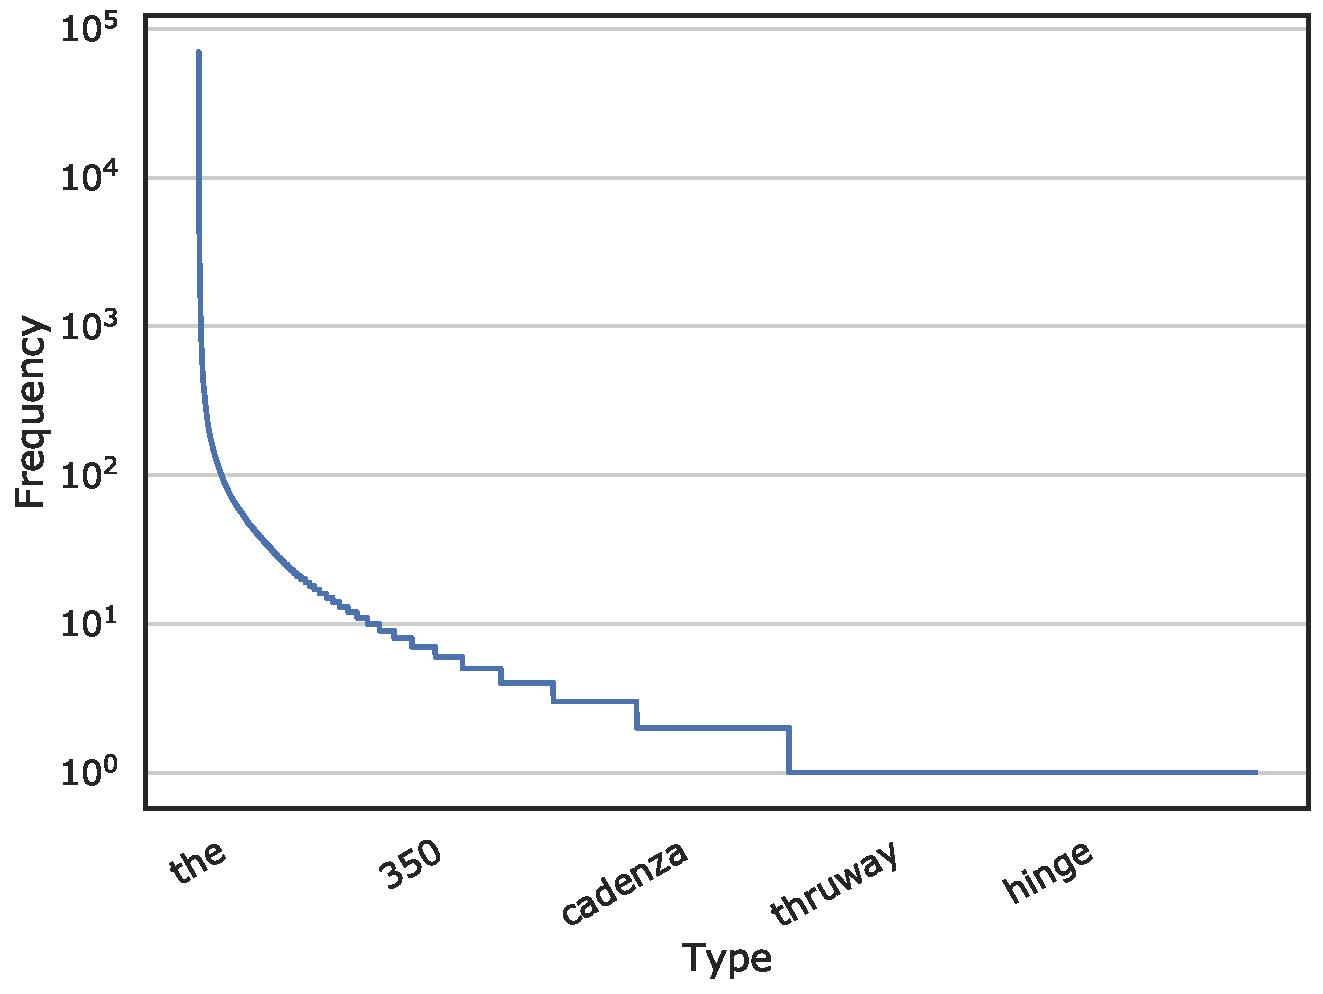
\includegraphics[width=0.75\textwidth]{img/background/brown-corpus-zipf.pdf}
    
    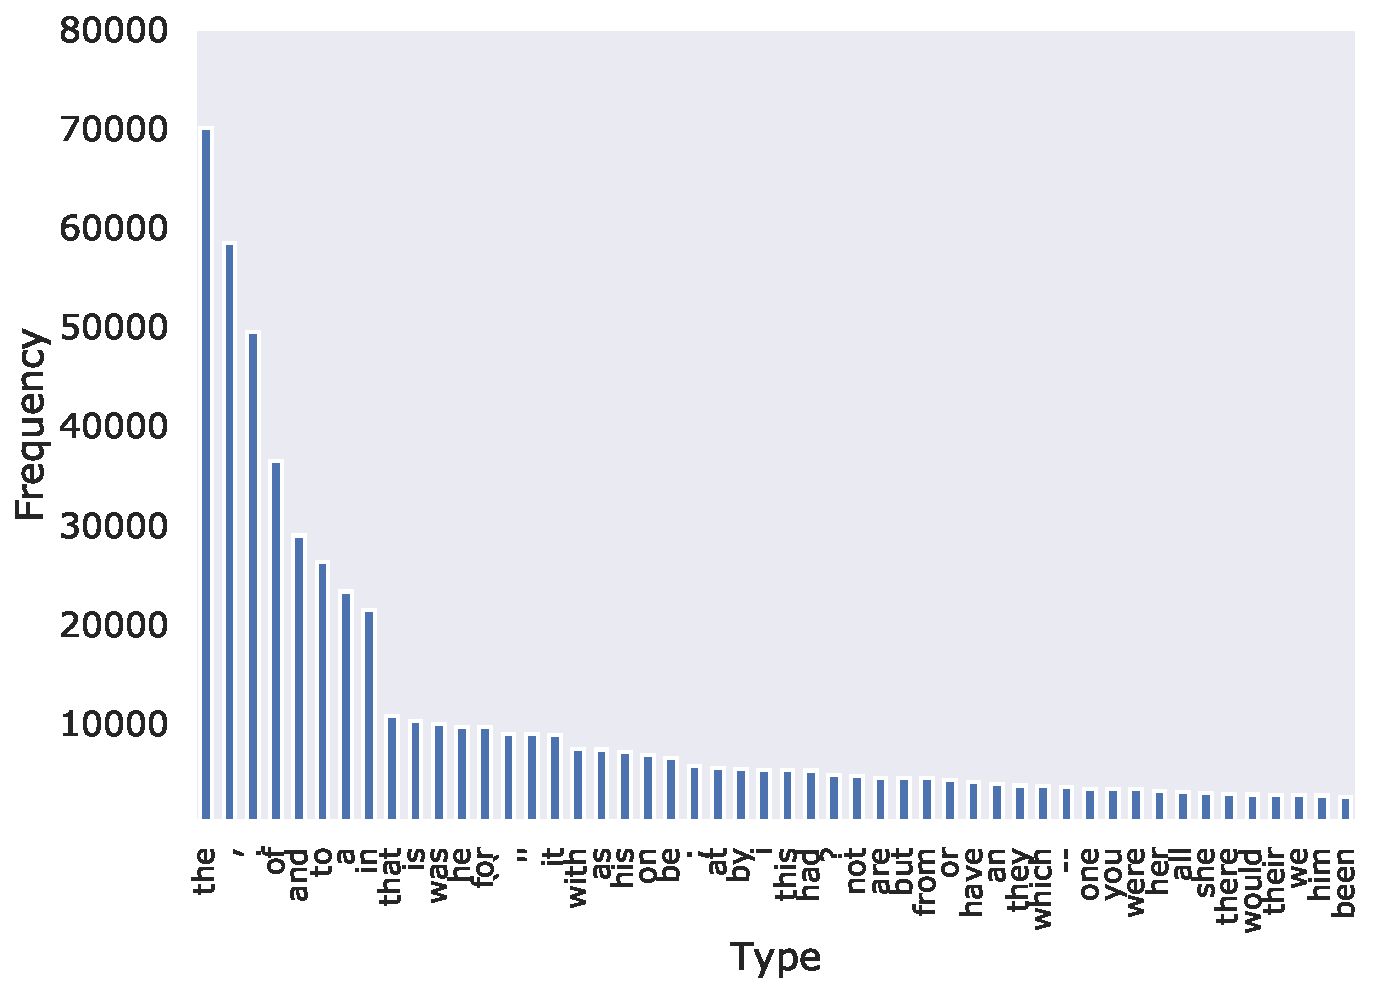
\includegraphics[width=0.75\textwidth]{img/background/brown-corpus-zipf-top50.pdf}
    \caption{Caption}
    \label{fig:my_label}
\end{figure}
\begin{figure}[ht]
    \centering
    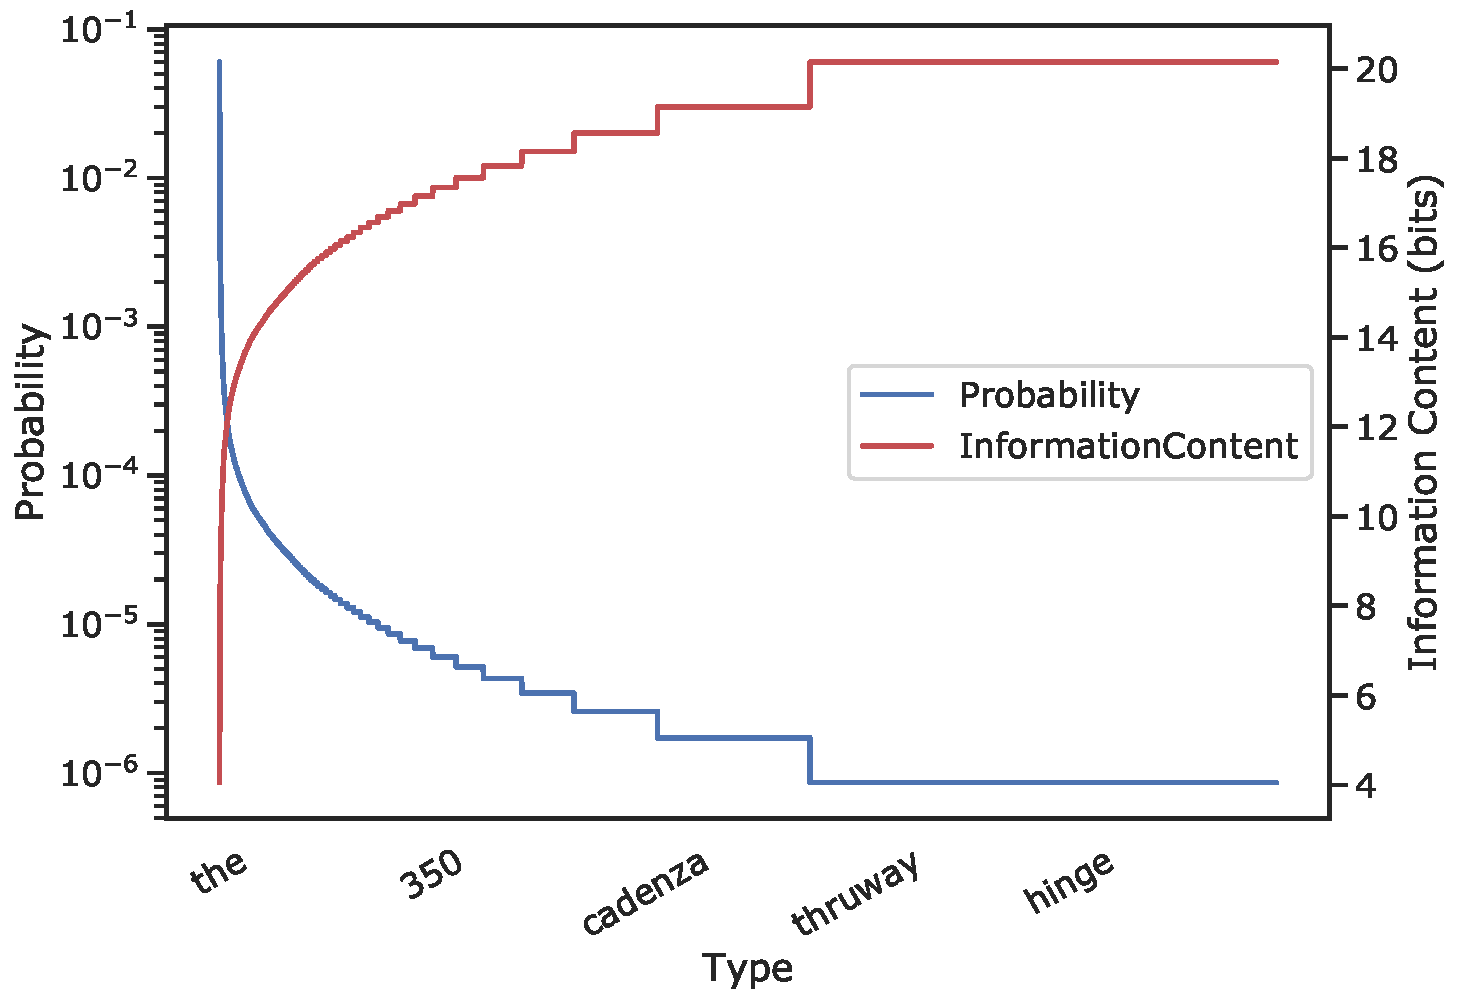
\includegraphics[width=0.75\textwidth, trim={3mm 0 3mm 0}, clip] {img/background/brown-corpus-shannons.pdf}
    \caption{Caption}
    \label{fig:my_label}
\end{figure}


%%---- COMMENT -----
\begin{comment}
Consider rare type translation: when the source and the target languages use the same alphabet,
%e.g. Romance languages such as English, French, Spanish, German, etc,
the rare types such as proper nouns and numeric types are often cognates which can be simply copied from the source to the target side without translation or transliteration. 
Shared vocabulary with tied embeddings which is widely used in the current translation models exploit this phenomenon ~\cite{press-wolf-2017-embeddings,vaswani2017attention}.
However, when translating between languages of heterogeneous scripts, rare word translation is more problematic.
Though techniques such as byte-pair-encoding \cite{sennrich-etal-2016-bpe} alleviate this problem, it is not entirely resolved ~\cite{gowda-may-2020-finding}.

\begin{figure}
    \centering
    \includegraphics[width=\linewidth]{img/gtranslate-error2.png}
    \caption{An example error from Google Translate {\footnotesize (accessed: June 15, 2021)}: `984' (in Kannada script) is translated to `2' in English; `984' is the crucial information in this example sentence.}
    \label{fig:gtrans-err}
\end{figure}
\end{comment}

%%---- COMMENT -----

\textbf{Proposal:} We propose to study and advance the following research arenas:
\begin{enumerate}
 \item How is class imbalance affecting NLG?
 \item Are the current NLG evaluation metrics addressing class imbalance? If not, how to create a metric that address imbalance?
 \item How to improve NLG performance in the light of imbalance?
\end{enumerate}

%We aim to study imbalanced learning under the realm of neural machine translation (NMT) task, however, since classifier is entangled with an autoregressor in NMT, certain imbalance learning strategies such as over-sampling and under-sampling are not directly applicable. 
%Imbalanced learning is widely studied under clearly defined classification tasks such as image classification. 

\chapter{Machine Learning Classification Modeling}

TODO:
1. Classification: traditional and deep learning
2. Traditional: naive bayes, SVM, decision trees, ...
3. Deep learning models: feed forward nets, RNNs, CNNs, Transformers, 


Machine learning is a field of study that enables creation of machines capable of learning from data instead of explicitly programming them.

Training and Prediction. \\ 
Random variables - discrete and continuous. -- Classification and Regression \\
Sometimes we convert continuous variables into discrete variables, e.g. quantization \\

Classification: binary and multi-class.  Single-label vs multi-label.



\section{NMT}
\subsection{NMT Architectures}
\label{sec:rel-nmt-arch}
Several variations of NMT models have been proposed and refined: \citet{sutskever2014seq2seq} and \citet{cho2014learning} introduce the RNN-based encoder-decoder model. 
\citet{bahdanau2014nmtattn} introduce the attention mechanism and \citet{luong2015effectiveAttn} propose several variations that became essential components of many future models.
RNN modules, either LSTM \cite{hochreiter1997LSTM} or GRU \cite{cho-etal-2014-properties}, have been popular choices for composing NMT encoders and decoders. 
The encoder uses bidirectional information, but the decoder is unidirectional, typically left-to-right, to facilitate autoregressive generation.
\citet{gehring2017CNNMT} use a CNN architecture that outperforms RNN models.
\citet{vaswani2017attention} propose the \textbf{Transformer}, whose main components are feed-forward and attention networks. 
There are only a few models that perform non-autoregressive NMT \cite{libovicky-helcl-2018-end,Gu-etal-17-NonAR-NMT}.
These are focused on improving the speed of inference; generation quality is currently sub-par compared to autoregressive models.
These non-autoregressive models can also be viewed as token classifiers with a different kind of feature extractor, whose strengths and limitations are yet to be theoretically understood.

\chapter{Rare Words at Training: Finding the Optimal Vocabulary}
\label{ch:nlg-imbalance}
%\section{Introduction}

Natural language processing tasks such as sentiment analysis \cite{maas-etal-2011-imdbreview, Zhang-etal-15-cnn-sentiment} and spam detection are modeled as classification tasks, where instances are independently labeled.
%\cite{CoNLL2017-shared-UD}
Tasks such as part-of-speech tagging and named entity recognition \cite{CoNLL-2003-NER} are examples of structured classification tasks, where instance classification is decomposed into a sequence of per-token contextualized labels.
We can similarly cast NMT, an example of a natural language generation task, as a form of structured classification, where an instance label (a translation) is generated as a sequence of contextualized labels, here by an autoregressor (see Section \ref{sec:classifier-nlg}).

Since the parameters of ML classification models are estimated from training data, whatever biases exist in the training data will affect model performance.
Among those biases, \textit{class imbalance} is a topic of our interest. 
Class imbalance is said to exist when one or more classes are not of approximately equal frequency in data.
%\change{this is good earlier in the intro in place of too much variable introduction}
The effect of class imbalance has been extensively studied in several domains where classifiers are used (see Section \ref{sec:rel-class-imb}).
With neural networks, the imbalanced learning problem is mostly targeted to computer vision tasks such as image segmentation; NLP tasks are under-explored \cite{Johnson2019SurveyImbalance}. 
% However neural networks are being used for many domains including NLP. 
 
Word types in natural language models resemble a Zipfian distribution, i.e., in any natural language corpus, we observe that a type's rank is roughly inversely proportional to its frequency. Thus, a few types are extremely frequent, while most of the rest lie on the long tail of infrequency. 
Zipfian distributions cause two problems in classifier-based NLG systems:
\begin{enumerate}
    \itemsep0em 
    \item \textbf{Unseen Vocabulary:} 
    Any hidden data set may contain types not seen in the finite set used for training. A sequence of words drawn from a Zipfian distribution is likely to have many rare types, and these are likely to have not been seen in training\cite{kornai2002many}. 
    \item \textbf{Imbalanced Classes:} There are a few extremely frequent types and many infrequent types, causing an extreme imbalance.  
    Such an imbalance, in other domains where classifiers are used, is known to cause undesired biases and severe performance degradation \cite{Johnson2019SurveyImbalance}. 
\end{enumerate} 

The use of \textit{subwords}, that is, decomposition of word types into pieces, such as the widely used Byte Pair Encoding (BPE) \cite{sennrich-etal-2016-bpe} addresses the open-ended vocabulary problem by ultimately allowing a word to be represented as a sequence of characters if necessary.
BPE has a single hyperparameter named \textit{merge operations} that governs the vocabulary size. 
The effect of this hyperparameter is not well understood. 
In practice, it is either chosen arbitrarily or via trial-and-error \cite{DBLP:journals/corr/abs-1810-08641}.

Regarding the problem of imbalanced classes, \citet{steedman-2008-last} states that ``\textit{the machine learning techniques that we rely on are actually very bad at inducing systems for which the crucial information is in rare events.}'' 
%They foresaw that \textit{``one day, either because of the demise of Moore’s law, or simply because we have done all the easy stuff, the Long Tail will comeback to haunt us"}.
However, to the best of our knowledge, this problem has not yet been directly addressed in the NLG setting.

In this chapter, we attempt to find answers to these questions: \textit{`What value of BPE vocabulary size is best for NMT?'}, and more crucially an explanation for \textit{`Why that value?'}.
As we will see, the answers and explanations for those are an immediate consequence of a broader question, namely \textit{`What is the impact of Zipfian imbalance on classifier-based NLG?'}

The organization of this chapter is as follows:
We offer a simplified view of NMT architectures by re-envisioning them as two high-level components: a \textit{classifier} and an \textit{autoregressor} (Section~\ref{sec:classifier-nlg}).
We describe some desired settings for the classifier (Section~\ref{sec:classifier-balance}) and autoregressor (Section~\ref{sec:ar-short-seq}) components.
In Section~\ref{sec:bpe}, we describe how vocabulary size choice relates to the desired settings for the two components. 
Our experimental setup is described in Section~\ref{sec:exp-setup}, followed by an analysis of results in Section~\ref{sec:nmt_analysis} that offers an explanation with evidence for \textit{why} some vocabulary sizes are better than others.  
Section~\ref{sec:class-bias} uncovers the impact of class imbalance, particularly frequency based discrimination on classes.\footnote{In this chapter, `type' and `class' are used interchangeably.}
% Section~\ref{sec:related-work} provides an overview of  related work, and in 
In Section~\ref{sec:conclusion}, we recommend a heuristic for choosing the BPE hyperparameter.

%%%%%%%%%%%%%%%%%%%%%%%%%%%%%%%%%%%%%%%%%%%%%%%%%%%%%%%%%%%%%%%%%%%%%%%%%%%%%%%%%%%%%%%%%%%%%%%
\section{Classifier based NLG}
\label{sec:classifier-nlg}

As discussed in Chapter \ref{ch:ml-background}, MT is the task of transforming sequences from the form $x = x_1 x_2 x_3 ... x_m$ to $y = y_1 y_2 y_3 ... y_n$, where, $x$ is in source language $X$ and $y$ is in target language $Y$. 
There are many variations of NMT architectures, however, all share the common objective of maximizing ${ \prod_{t=1}^{n} P(y_t | y_{<t}, x_{1:m})}$ for pairs $(x_{1:m}, y_{1:n})$ sampled from a parallel dataset. 
NMT architectures are commonly viewed as encoder-decoder networks.
We instead re-envision the NMT architecture as two higher level components: an autoregressor ($R$) and a multi-class classifier ($C$), as shown in Figure~\ref{fig:nmt-architecture}.
\begin{figure}[ht]
    \centering
    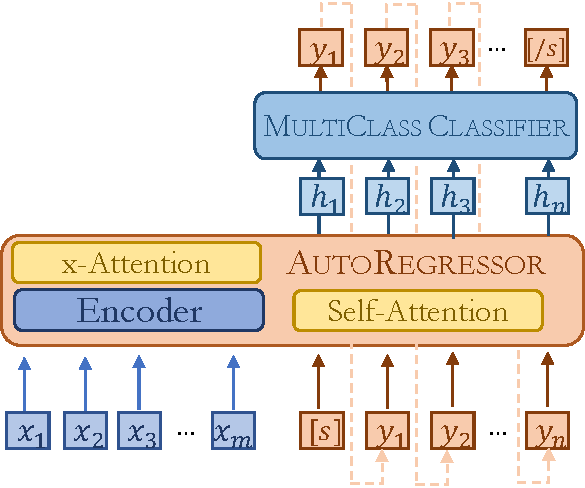
\includegraphics[width=0.65\linewidth]{img/optimvocab/nmt-arch-classifier-new}
    \caption{The NMT model re-envisioned as a token classifier with an autoregressive feature extractor.}
    \label{fig:nmt-architecture}
%% to edit this, go to https://docs.google.com/drawings/d/1Ei9m3WanLJRvoegurFZpiSRQTz7p1Mmde25G0ZwnmAU/edit 
\end{figure}

Autoregressor $R$, \cite{box2015time} being the most complex component of the NMT model, has many implementations based on various neural network architectures: recurrent neural networks (RNN) such as long short-term memory (LSTM) and gated recurrent unit (GRU), convolutional neural networks (CNN), and Transformer. 
At time step $t$, $R$ transforms the input context $y_{<t}, x_{1:m}$ into hidden state vector $h_t = R(y_{<t}, x_{1:m})$.

Classifier $C$ is the same across all architectures.
It maps $h_t$ to a distribution $P(y_j | h_t) \forall y_j \in V_Y$, where $V_Y$ is the vocabulary of $Y$. 
Input to classifiers such as $C$ is generally described as features that are either hand-engineered or automatically extracted.
In our high-level view of NMT architectures, $R$ is a neural network that serves as an automatic feature extractor for $C$.

\subsection{Balanced Classes for Token Classifier}
\label{sec:classifier-balance}

Untreated, class imbalance leads to bias based on class frequencies.
Specifically, classification learning algorithms focus on frequent classes while paying relatively less importance to infrequent classes.
Frequency-based bias leads to poor recall of infrequent classes \cite{Johnson2019SurveyImbalance}. 

When a model is used in a \textit{domain mismatch} scenario, i.e., where test and training set distributions do not match, model performance generally degrades.
It is not surprising that frequency-biased classifiers show particular degradation in domain mismatch scenarios, as  types that were infrequent in the training distribution and were ignored by the learning algorithm may appear with high frequency in the new domain.
\citet{koehn2017sixchallenges} showed empirical evidence of poor generalization of NMT to out-of-domain datasets.

In other classification tasks, where each instance is classified independently, methods such as up-sampling infrequent classes and down-sampling frequent classes are used.
In NMT, since classification is done within the context of sequences, it is possible to accomplish the objective of balancing by altering sequence lengths.
This can be done by choosing the level of subword segmentation \cite{sennrich-etal-2016-bpe}.

\textbf{Quantification of Zipfian Imbalance:}
We use two statistics to quantify the imbalance of a training distribution:

The first statistic relies on a measure of \textbf{Divergence} ($D$) from a balanced (uniform) distribution. 
We use a simplified version of Earth Mover Distance, in which the total cost for moving a probability mass between any two classes  is the sum of the total mass moved.
Since any mass moved \textit{out of} one class is moved \textit{into} another, we divide the total per-class mass moves in half to avoid double counting.  
Therefore, the imbalance measure $D$ on $K$ class distributions where $p_i$ is the observed probability of class $i$ in the training data is computed as:
$$D = \frac{1}{2} \sum_{i=1}^{K}| p_i - \frac{1}{K}|; \quad 0 \le D \le 1 $$

A lower value of $D$ is the desired setting for $C$, since the lower value results from a balanced class distribution. 
When classes are balanced, they have approximately equal frequencies; $C$ is thus less likely to make errors due to class bias.

The second statistic is \textbf{Frequency at 95th\% Class Rank (\textbf{$F_{95\%}$})}, defined as the least frequency in the $95^{th}$ percentile of most frequent classes.
More generally, $F_{\large{P\%}}$ is a simple way of quantifying the minimum number of training examples for at least the $P$th percentile of classes.
The bottom $(1-P)$ percentile of classes are ignored to avoid the noise that is inherent in the real-world natural-language datasets.

A higher value for $F_{95\%}$ is the desired setting for $C$, as a higher value indicates the presence of many training examples per class, and ML methods are known to perform better when there are many examples for each class.  


\subsection{Shorter Sequences for Autoregressor}
\label{sec:ar-short-seq}

Every autoregressive model is an approximation; some may be better than others, but no model is perfect. 
The total error accumulated grows in proportion to the length of the sequence.
These accumulated errors alter the prediction of subsequent tokens in the sequence.
Even though beam search attempts to mitigate this, it does not completely resolve it.  
These challenges with respect to long sentences and beam size are examined by \citet{koehn2017sixchallenges}.


We summarize sequence lengths using \textbf{Mean Sequence Length}, $\mu$, 
computed trivially as the arithmetic mean of the lengths of \textit{target} language sequences after encoding them:
$\mu = \frac{1}{N} \sum_{i=1}^N |y^{(i)}|$
where $y^{(i)}$ is the $i$th sequence in the training corpus of $N$ sequences.
Since shorter sequences have relatively fewer places where an imperfectly approximated autoregressor model can make errors, a smaller $\mu$ is a desired setting for $R$.

%%%%%%%%%%%%%%%%%%%%%%%%%%%%%%%%%%%%%%%%%%%%%%%%%
\subsection{Choosing the Vocabulary Size Systematically}
\label{sec:bpe}

BPE~\cite{sennrich-etal-2016-bpe} is a greedy iterative algorithm often used to segment a vocabulary into useful \textit{subwords}. 
The algorithm starts with characters as its initial vocabulary.
In each iteration, it greedily selects the most frequent type bigram in the training corpus, and replaces the sequence with a newly created compound type.
Once the subword vocabulary is learned, it can be applied to a corpus by greedily segmenting words with the longest available subword type. These operations have an effect on $D$, $F_{95\%}$, and $\mu$.

\textbf{Effect of BPE on $\mu$}:
BPE expands rare words into two or more subwords, lengthening a sequence (and raising $\mu$) relative to simple white-space segmentation.
BPE merges frequent-character sequences into one subword piece, shortening a sequence (and lowering $\mu$) relative to character segmentation.
Hence, the sequence length of BPE segmentation lies in between the sequence lengths obtained by white-space and character-only segmentation methods \cite{morishita-etal-2018-improving}. 

\textbf{Effect of BPE on $F_{95\%}$ and $D$}:
Whether BPE is viewed as a merging of frequent subwords into a relatively less frequent compound, or a splitting of rare words into relatively frequent subwords, BPE alters the class distribution by moving the probability mass of classes.
Hence, by altering the class distribution, BPE also alters both $F_{95\%}$ and $D$. The BPE hyperparameter controls the amount of probability mass moved between subwords and compounds.

Figure~\ref{fig:BPE-imbalance} shows the relation between number of BPE merges (i.e. the BPE hyperparameter), and both $D$ and $\mu$.
When few BPE merge operations are performed, we observe the lowest value of $D$, which is a desired setting for $C$, but at the same point $\mu$ is large and undesired for $R$ (Section~\ref{sec:classifier-nlg}).
When a large number of BPE merges are performed, the effect is reversed, i.e. we observe that $D$ is large and unfavorable to $C$ while $\mu$ is small and favorable to $R$. 
In the following sections we describe our experiments and analysis to locate the optimal number of BPE merges that achieves the right trade-off for both $C$ and $R$. 

 \begin{figure}[ht]
  \centering
    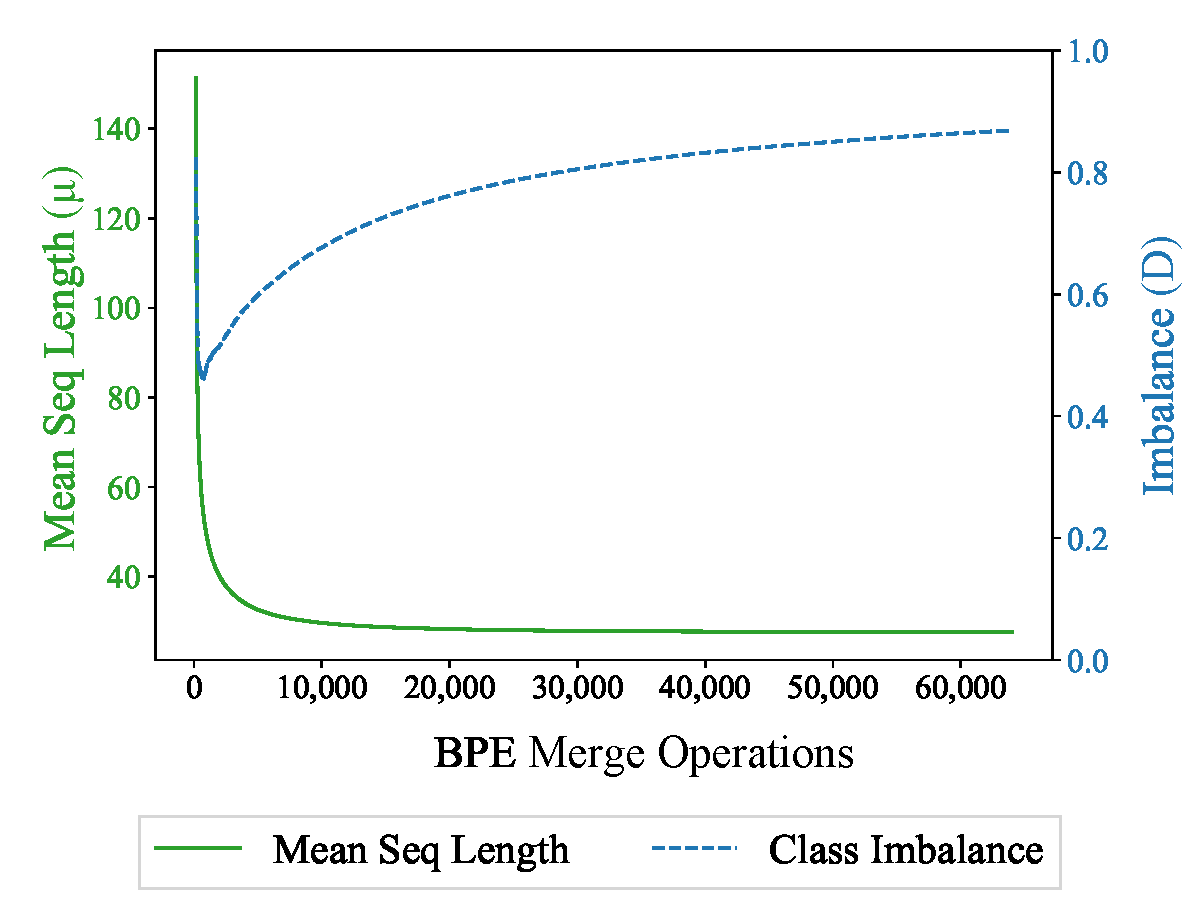
\includegraphics[width=0.7\linewidth]{bpe64k-deen-en.pdf}
    \caption{Effect of BPE merge operations on mean sequence length ($\mu$) and class imbalance ($D$).
    } 
    \label{fig:BPE-imbalance}
\end{figure}


\section{Experimental Setup}
\label{sec:exp-setup}

Our NMT experiments use the base Transformer model \cite{vaswani-2017-attention} on four different target languages at various training data sizes, described in the following subsections. 

\subsection{Datasets}
We use the following four language pairs for our analysis: English$\rightarrow$German, German$\rightarrow$English, English$\rightarrow$Hindi, and English$\rightarrow$Lithuanian. 
To analyze the impact of different training data sizes, we randomly sub-select smaller training corpora for English$\leftrightarrow$German and English$\rightarrow$Hindi language pairs. 
Statistics regarding the corpora used for validation, testing, and training are in Table~\ref{tab:datasets}.
The datasets for English$\leftrightarrow$German, and English$\rightarrow$Lithuanian are retrieved from the News Translation task of WMT2019~\cite{wmt19proceedings}.\footnote{\href{http://www.statmt.org/wmt19/translation-task.html}{http://www.statmt.org/wmt19/translation-task.html}}
For English$\rightarrow$Hindi, we use the IIT Bombay Hindi-English parallel corpus v1.5~\cite{kunchukuttan-etal-2018-iit}.
English, German, and Lithuanian sentences are tokenized using \textsc{SacreMoses}.\footnote{\href{https://github.com/alvations/sacremoses}{https://github.com/alvations/sacremoses}} 
Hindi sentences are tokenized using \textsc{IndicNlpLibrary}.\footnote{\href{https://github.com/anoopkunchukuttan/indic_nlp_library}{https://github.com/anoopkunchukuttan/indic\_nlp\_library}}

The training datasets are trivially cleaned: we exclude sentences with length in excess of five times the length of their parallel counterparts. 
Since the vocabulary is a crucial part of this analysis, we exclude all sentence pairs containing URLs. 

\begin{table*}[ht]
    \centering
    \setlength{\tabcolsep}{3pt}
\begin{tabular}{ l  : l  : r  r  r  : l : l }
  Languages & Training & Sentences & EN Toks & XX Toks & Validation & Test \\ \hline
\multirow{4}{1.5cm}{DE$\rightarrow$EN\\EN$\rightarrow$DE} 
    & \multirow{4}{4cm}{Europarl v10 \\ WMT13CommonCrawl \\ NewsCommentary v14}
         & 30K  &  0.8M & 0.8M & \multirow{4}{*}{ {\small NewsTest18} }
            & \multirow{4}{*}{ \small{NewsTest19}} \\ \cdashline{3-5}
    &    & 0.5M  & 12.9M & 12.2M &  &  \\ \cdashline{3-5}
    &    & 1M    & 25.7M & 24.3M &  &  \\ \cdashline{3-5} 
    &    & 4.5M  & 116M & 109.8M &  &  \\ \hdashline

\multirow{2}{*}{EN$\rightarrow$HI } 
     & \multirow{2}{*}{ IITB Training } 
         & 0.5M & 8M & 8.6M  & \multirow{2}{*}{ \small{IITB Dev} } 
     & \multirow{2}{*}{ \small{IITB Test} }  \\\cdashline{3-5} 
     &   & 1.3M & 21M & 22.5M   &   &  \\ \hdashline 
EN$\rightarrow$LT & Europarl v10 & 0.6M & 17M & 13.4M  & \small{NewsDev19} & \small{NewsTest19} \\
\end{tabular} 
    \caption{Training, validation, and testing datsets, along with sentence and token counts in training sets. We generally refer to dataset's sentences as size in this chapter.}
    \label{tab:datasets}
\end{table*}

\subsection{Hyperparameters}
Our model is a 6 layer Transformer encoder-decoder that has 8 attention heads, 512 hidden vector units, and a feed forward intermediate size of 2048, with GELU activation. 
We use label smoothing at 0.1, and a dropout rate of 0.1.
We use the Adam optimizer \cite{kingma2015adam} with a controlled learning rate that warms up for 16K steps followed by the decay rate recommended for training Transformer models~\cite{popel2018tfm-train-tips}. 
To improve performance at different data sizes, we set the mini-batch size to 6K tokens for the 30K-sentence datasets, 12K tokens for 0.5M-sentence datasets, and 24K for the remaining larger datasets~\cite{popel2018tfm-train-tips}. 
All models are trained until no improvement in validation loss is observed, with patience of 10 validations, each done at 1,000 update steps apart. 
Our model is implemented using PyTorch and run on NVIDIA P100 and V100 GPUs.
To reduce padding tokens per batch, mini-batches are made of sentences having similar lengths \cite{vaswani-2017-attention}.
We trim longer sequences to a maximum of 512 tokens after BPE.
To decode, we average the last 10 checkpoints, and use a beam size of 4 with length penalty of 0.6, similar to \citet{vaswani-2017-attention}.

Since the vocabulary size hyperparameter is the focus of this analysis, we use a range of vocabulary sizes that include character vocabulary and BPE operations that yield vocabulary sizes between 500 and 64K types.
A common practice, as seen in \citet{vaswani-2017-attention}'s setup, is to jointly learn BPE for both source and target languages, which facilitates three-way weight sharing between the encoder's input, the decoder's input, and the output (i.e., classifier's class) embeddings \cite{press-wolf-2017-embeddings}.
However, to facilitate fine-grained analysis of vocabulary sizes and their effect on class imbalance, our models separately learn source and target vocabularies; weight sharing between the encoder's and decoder's embeddings is thus not possible.
For the target language, however, we share weights between the decoder's input and the classifier's class embeddings.

\section{Results and Analysis}
\label{sec:nmt_analysis}

\begin{figure}[h!t]
\centering
\begin{subfigure}{\linewidth}
    \centering
    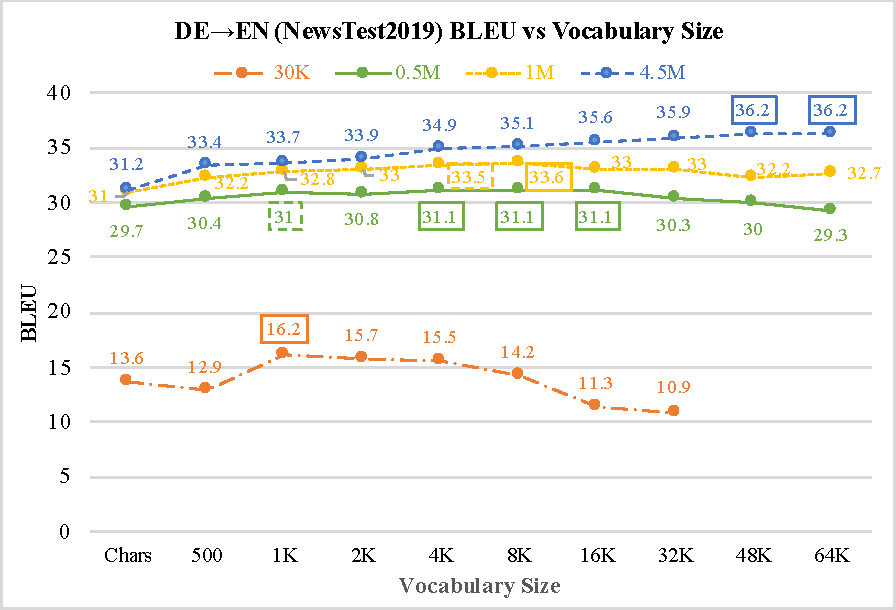
\includegraphics[width=0.7\linewidth]{bleu-deen.pdf}
    \caption{DE$\rightarrow$EN BLEU on NewsTest2019}
    \label{fig:bleu-deen}
\end{subfigure}

\vspace{5mm}

\begin{subfigure}{\linewidth}
    \centering
    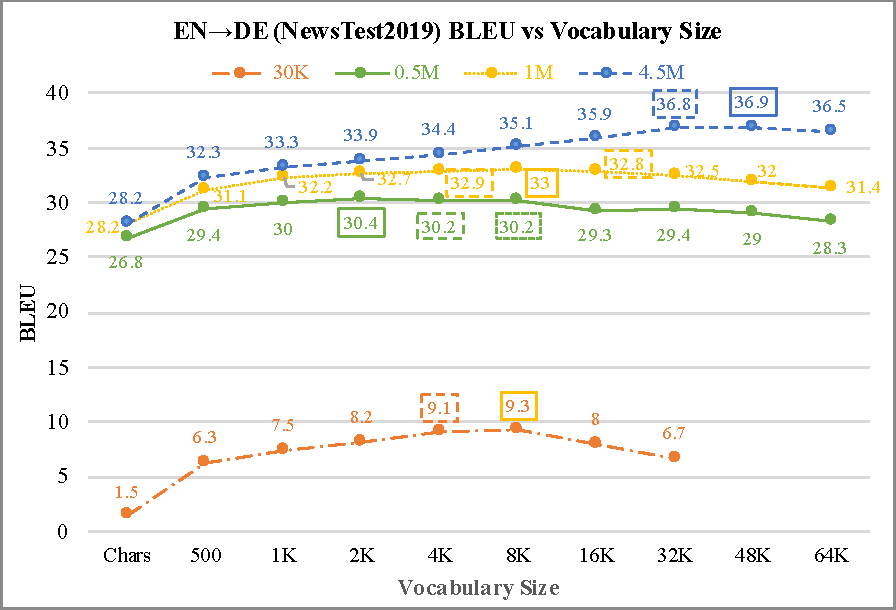
\includegraphics[width=0.7\linewidth]{bleu-ende.pdf}
    \caption{EN$\rightarrow$DE BLEU on NewsTest2019}
    \label{fig:bleu-ende}
\end{subfigure}
\caption{EN$\leftrightarrow$DE NewsTest2019 BLEU as a function of vocabulary size at various training set sizes. 
Only the large dataset with 4.5M sentences has its best performance at a large vocabulary; all others peak at an 8K or smaller vocabulary size.}
\label{fig:bleu-ende-deen}
\end{figure}

\begin{figure}[ht]
    \centering    
    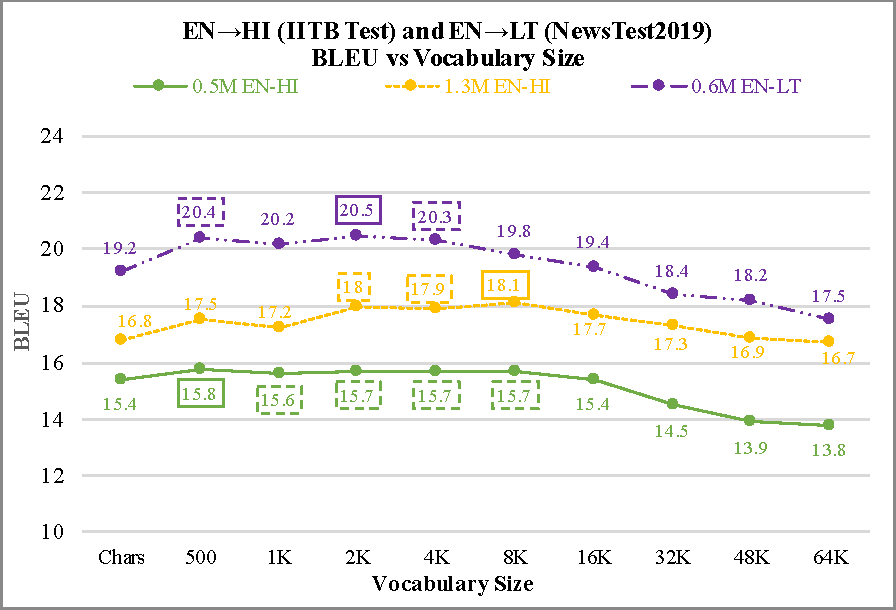
\includegraphics[width=0.7\linewidth]{bleu-enhi-enlt.pdf}
    \caption{BLEU on EN$\rightarrow$HI IITB Test and EN$\rightarrow$LT NewsTest2019 as a function of vocabulary size.
    These language pairs observed the best BLEU scores in the range of 500 to 8K vocabulary size.}
    \label{fig:bleu-enhilt}
\end{figure}

BLEU scores for DE$\rightarrow$EN and EN$\rightarrow$DE experiments are reported in Figures~\ref{fig:bleu-deen} and \ref{fig:bleu-ende} respectively.
Results from EN$\rightarrow$HI, and EN$\rightarrow$LT are combined in Figure~\ref{fig:bleu-enhilt}.
All the reported BLEU scores are obtained using \textsc{SacreBleu} \cite{post-2018-sacrebleu}.\footnote{\texttt{BLEU+case.mixed+numrefs.1+smooth.exp+tok.13a+version.1.4.6}}

We make the following observations: smaller vocabulary such as characters have not produced the best BLEU for any of our language pairs or dataset sizes. 
A vocabulary of 32K or larger is unlikely to produce optimal results unless the data set is large e.g. the 4.5M DE$\leftrightarrow$EN sets.
The BLEU curves as a function of vocabulary sizes have a shape resembling a hill. 
The position of the peak of the hill seems to shift towards a larger vocabulary when the datasets are large. 
However, there is a lot of variance in the position of the peak: one extreme is at 500 types on 0.5M EN$\rightarrow$HI, and the other extreme is at 64K types in 4.5M DE$\rightarrow$EN. 
    
Although Figures~\ref{fig:bleu-ende-deen} and \ref{fig:bleu-enhilt} indicate \textit{where} the optimal vocabulary size is for these chosen language pairs and datasets, the question of \textit{why} the peak is where it is remains unanswered.
We visualize $\mu$, $D$, and $F_{95\%}$ in Figures \ref{fig:mu-d-freq-bleu} and \ref{fig:mu-d-freq-bleu-continued} to answer that question, and report these observations:
\begin{enumerate}
    \itemsep0em 
    \item Small vocabularies have a relatively larger $F_{95\%}$ (favorable to classifier), yet they are suboptimal. We reason that this is due to the presence of a larger $\mu$, which is unfavorable to the autoregressor.
    \item Larger vocabularies such as 32K and beyond have a smaller $\mu$, which favors the autoregressor, yet rarely achieves the best BLEU.
    We reason this is due to the presence of a lower $F_{95\%}$ and a higher $D$ being unfavorable to the classifier.
    Since the larger datasets have many training examples for each class, as indicated by a generally larger $F_{95\%}$, we conclude that bigger vocabularies tend to yield optimal results compared to smaller datasets in the same language.
    
    \item On small (30K) to medium (1.3M) data sizes, the vocabulary size of 8K seems to find a good trade-off between $\mu$ and $D$, as well as between $\mu$ and $F_{95\%}$.
\end{enumerate}

 There is a \textit{simple heuristic} to locate the peak: the near-optimal vocabulary size is where sentence length $\mu$ is small, while $F_{95\%}$ is approximately $100$ or higher.
 
 
 \begin{figure}[h!t]
    \centering
    \begin{subfigure}{0.8\textwidth}
    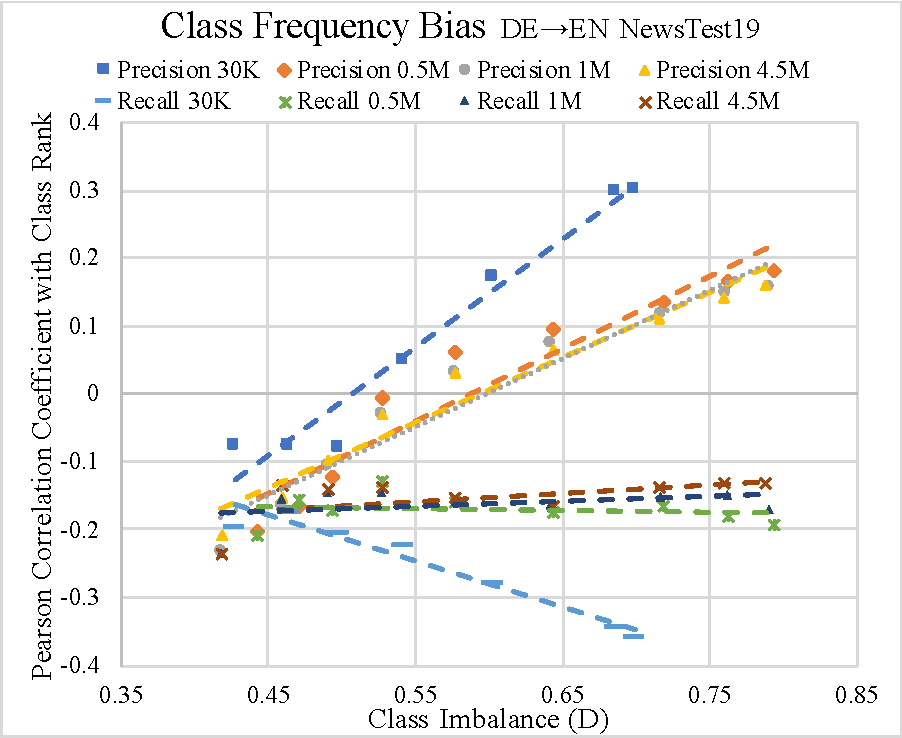
\includegraphics[width=\linewidth]{corr-deen-test.pdf}
    \end{subfigure}
    
    \vspace{5mm}

    \begin{subfigure}{0.8\textwidth}
    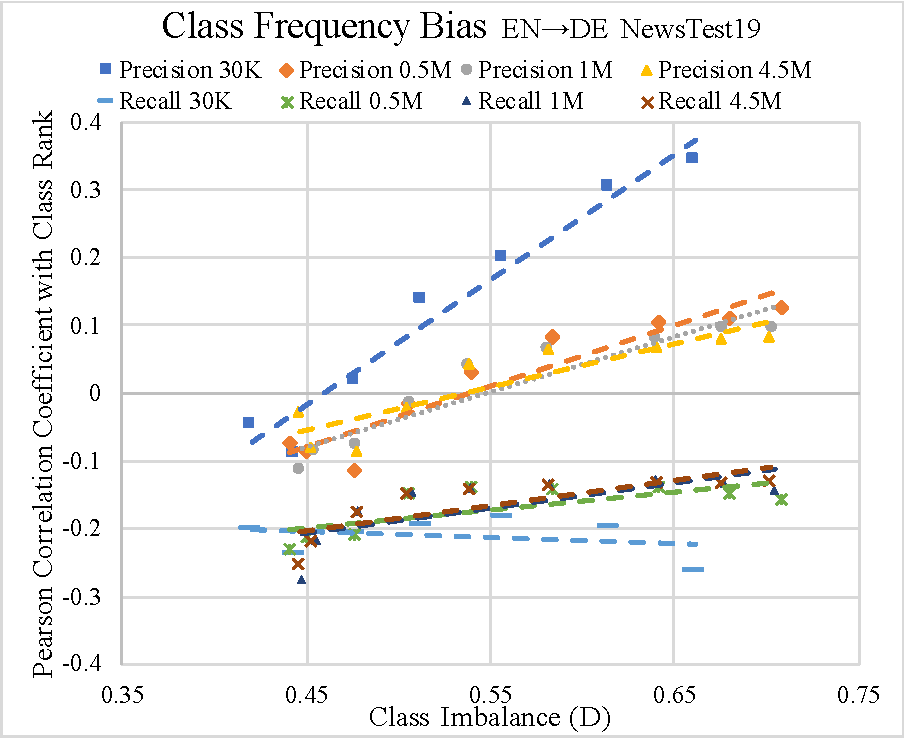
\includegraphics[width=\linewidth]{corr-ende-test.pdf}
    \end{subfigure}
    
    \caption{Correlation analysis on DE$\rightarrow$EN and EN$\rightarrow$DE shows that NMT models suffer from frequency based class bias, indicated by non-zero correlation of both precision and recall with class rank. Reduction in class imbalance (D), as shown by the horizontal axis, generally reduces the bias as indicated by the reduction in magnitude of correlation.}
         \label{fig:corr-deen-test}
\end{figure}
 
 

\begin{figure}[h!t]
\centering
\begin{subfigure}{\textwidth}
  \centering
  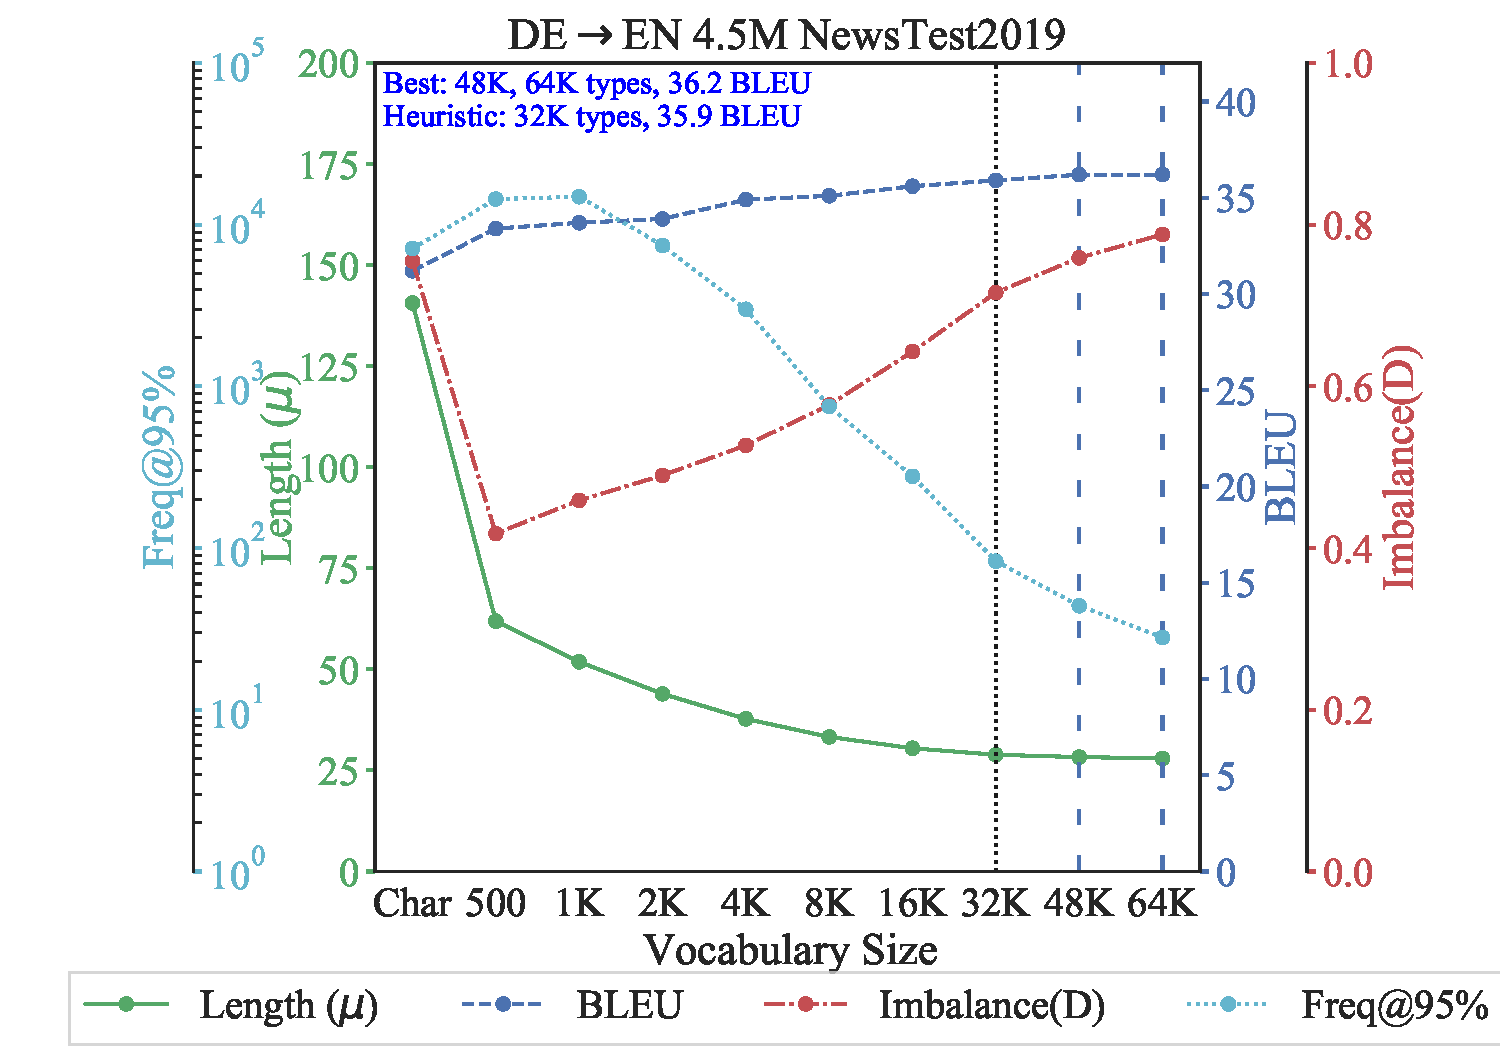
\includegraphics[width=0.7\linewidth,trim={1.4cm 0 0.2cm 16.45cm},clip]{4axv-test-deen-4.5m.pdf}
\end{subfigure}

\vspace{1mm}

\begin{subfigure}{.44\textwidth}
  \centering
  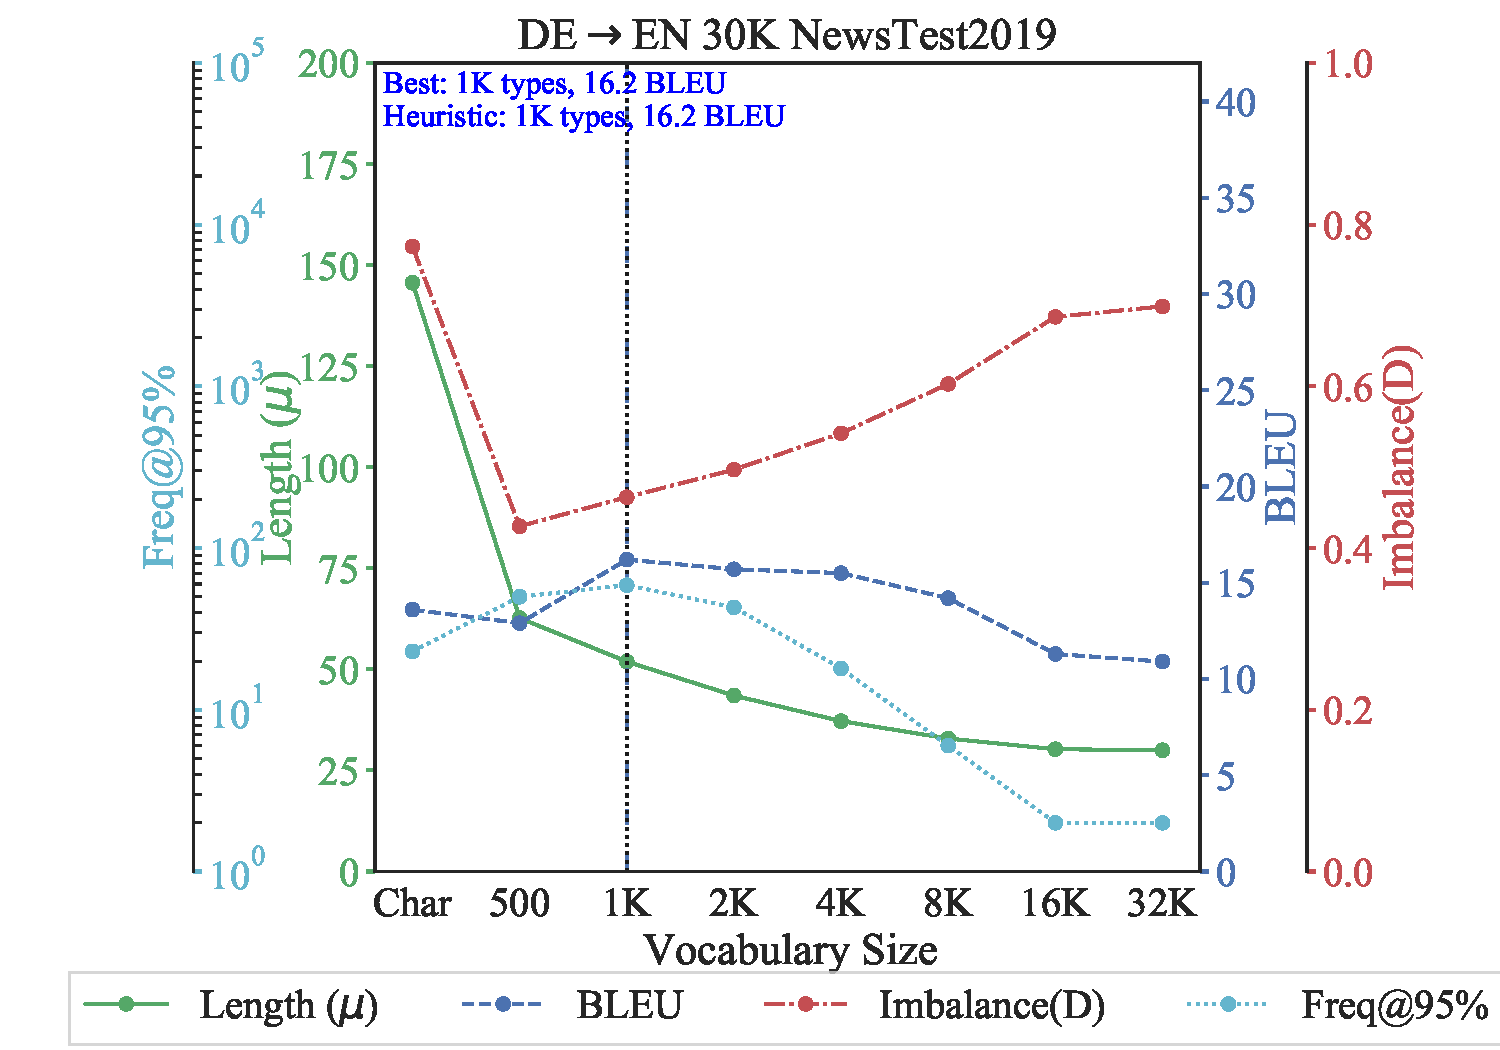
\includegraphics[width=0.99\linewidth,trim={2.4cm 1.32cm 4.1cm 0},clip]{4axv-test-deen-30k.pdf}
  %\caption{1a}
  %\label{fig:sfig1}
\end{subfigure}
\begin{subfigure}{.44\textwidth}
  \centering
  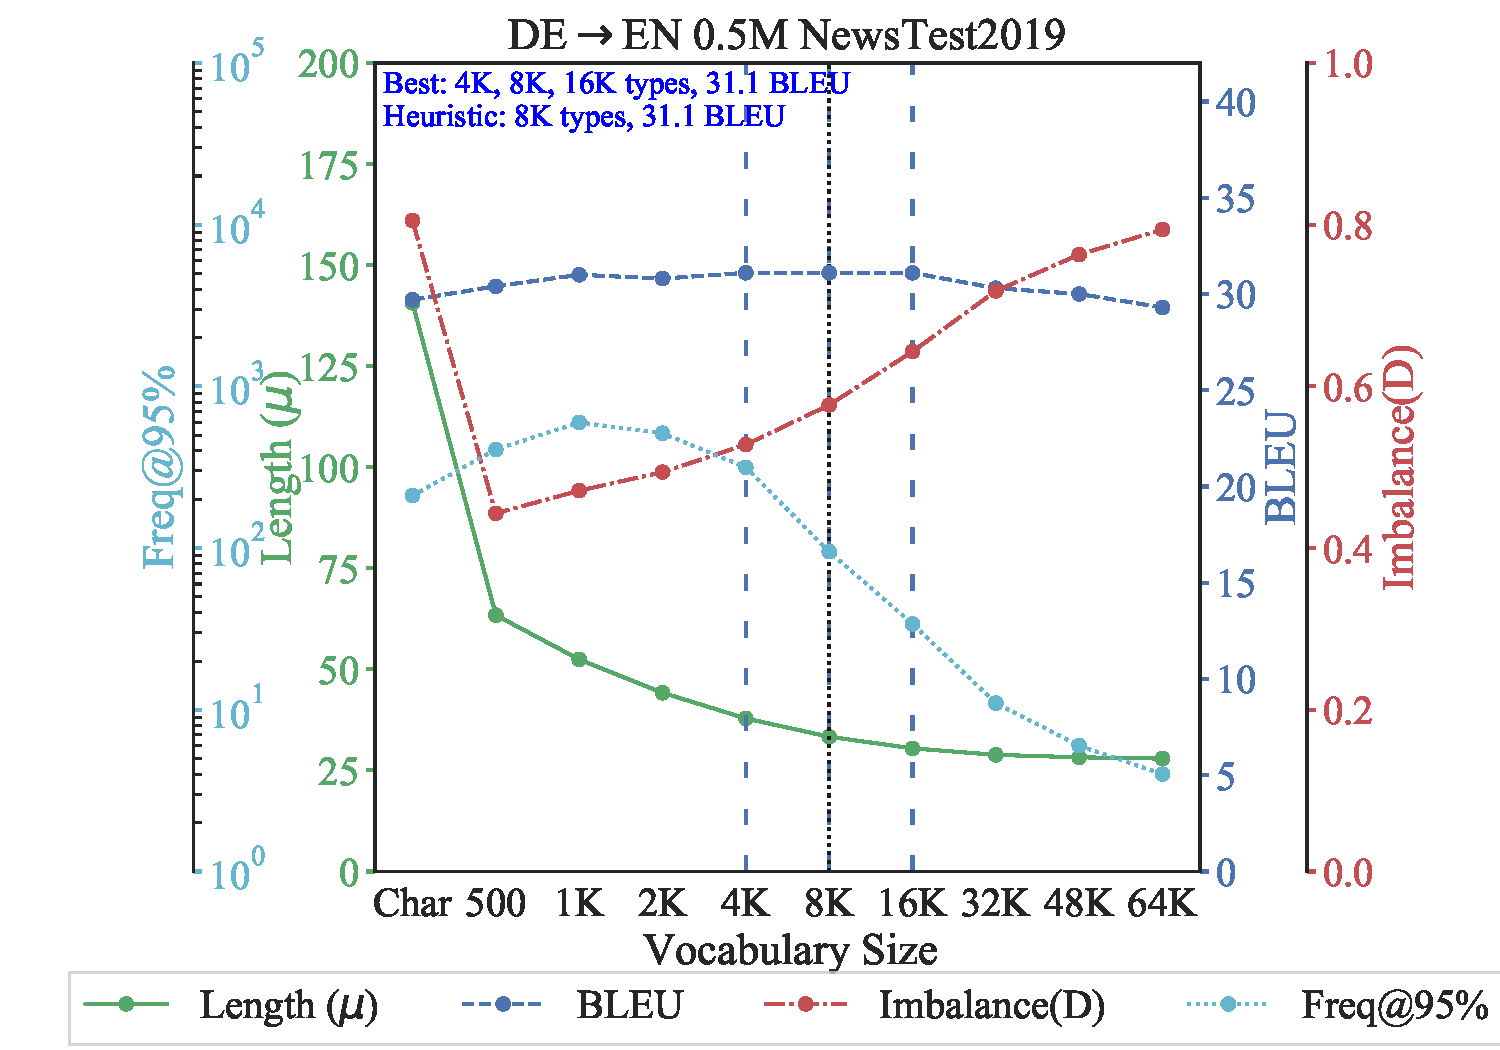
\includegraphics[width=0.99\linewidth,trim={5.1cm 1.32cm 1.4cm 0},clip]{4axv-test-deen-0.5m.pdf}
  %\caption{1c}
  %\label{fig:sfig2}
\end{subfigure}


\begin{subfigure}{.44\textwidth}
  \centering
  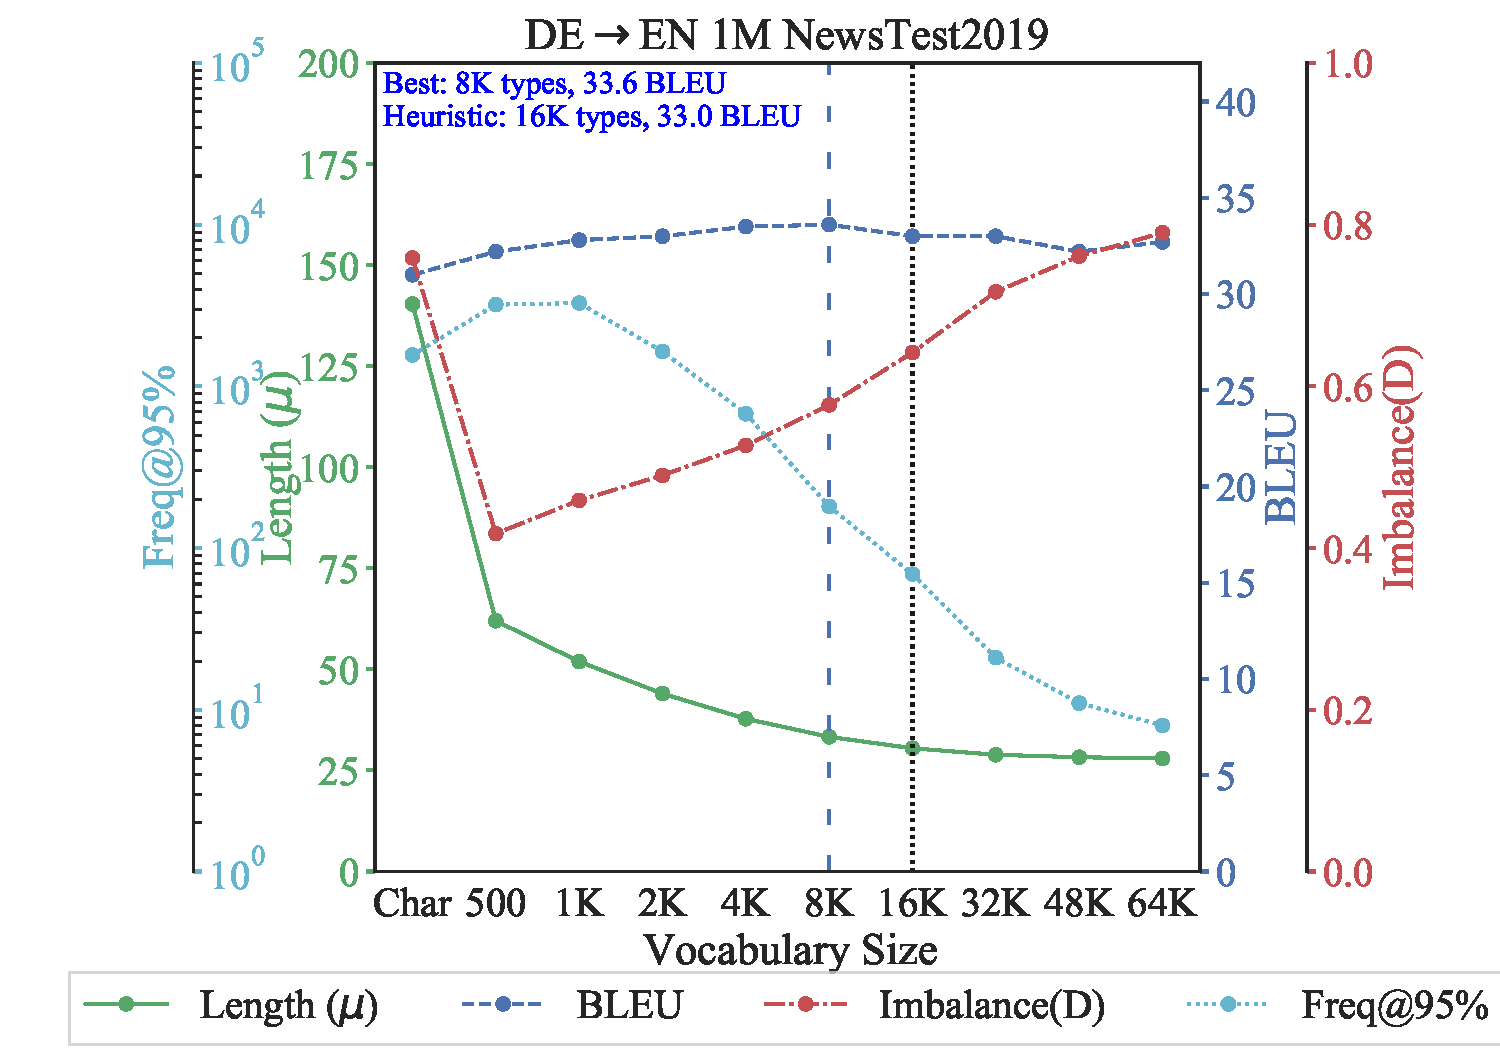
\includegraphics[width=0.99\linewidth,trim={2.4cm 1.32cm 4.1cm 0},clip]{4axv-test-deen-1m.pdf}
  %\caption{1c}
  %\label{fig:sfig2}
\end{subfigure}
\begin{subfigure}{.44\textwidth}
  \centering
  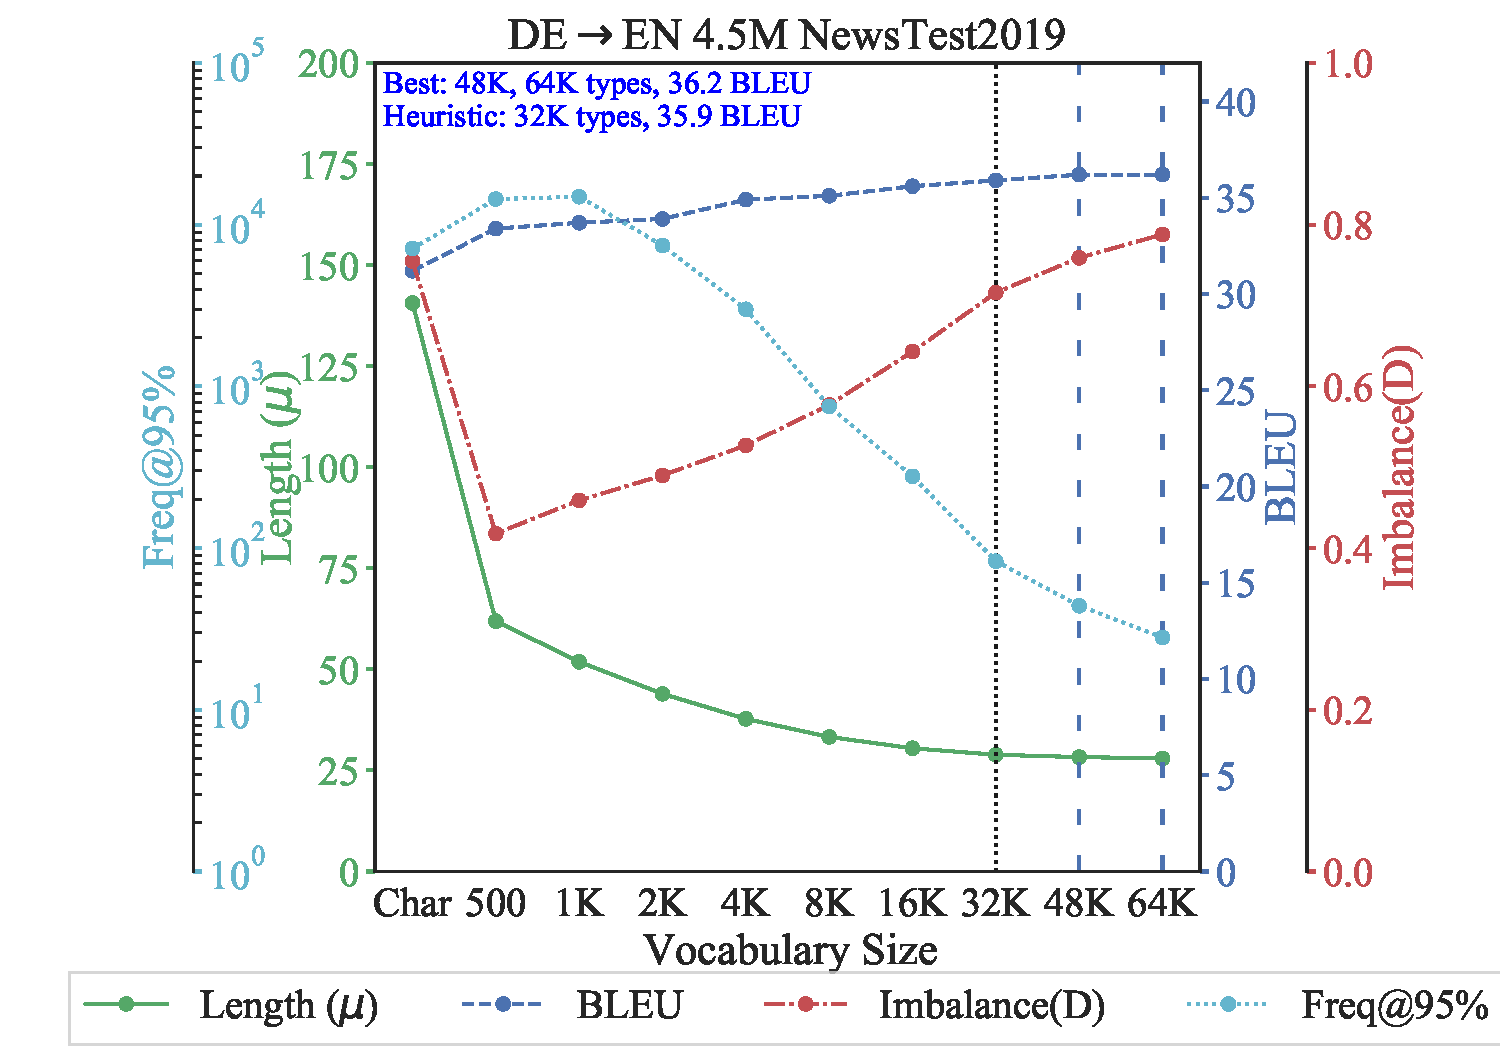
\includegraphics[width=0.99\linewidth,trim={5.1cm 1.32cm 1.4cm 0},clip]{4axv-test-deen-4.5m.pdf}
  %\caption{1c}
  %\label{fig:sfig2}
\end{subfigure}

\begin{subfigure}{.44\textwidth}
  \centering
  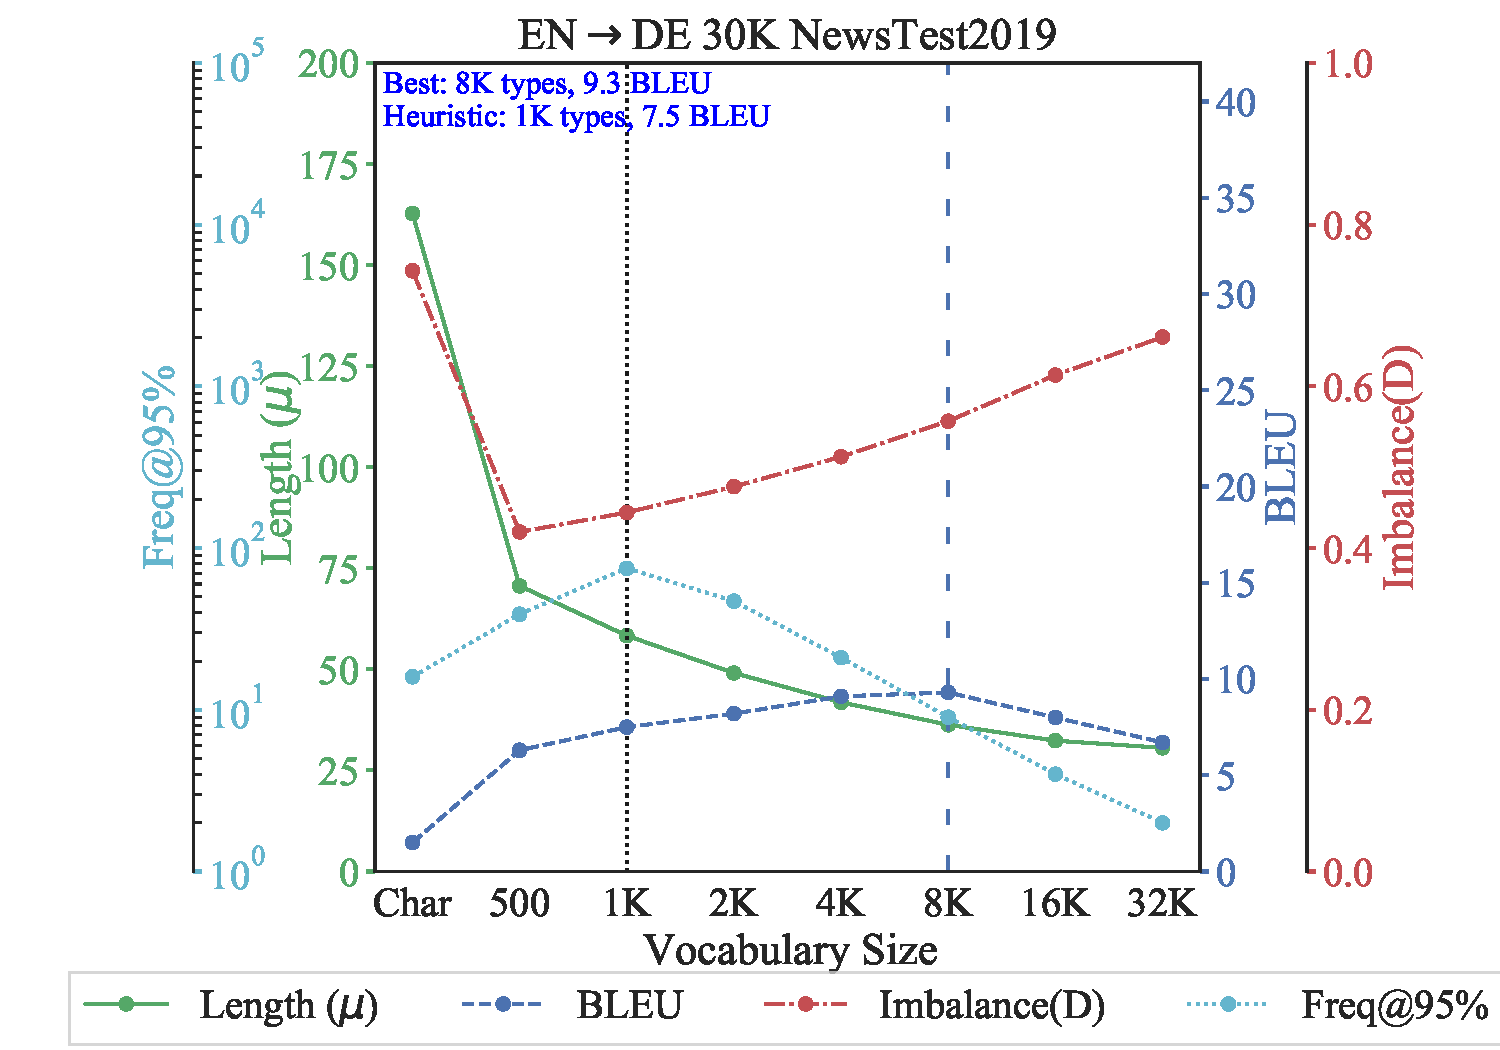
\includegraphics[width=0.99\linewidth,trim={2.4cm 1.32cm 4.1cm 0},clip]{4axv-test-ende-30k.pdf}
 % \caption{1a}
  %\label{fig:sfig1}
\end{subfigure}
\begin{subfigure}{.44\textwidth}
  \centering
  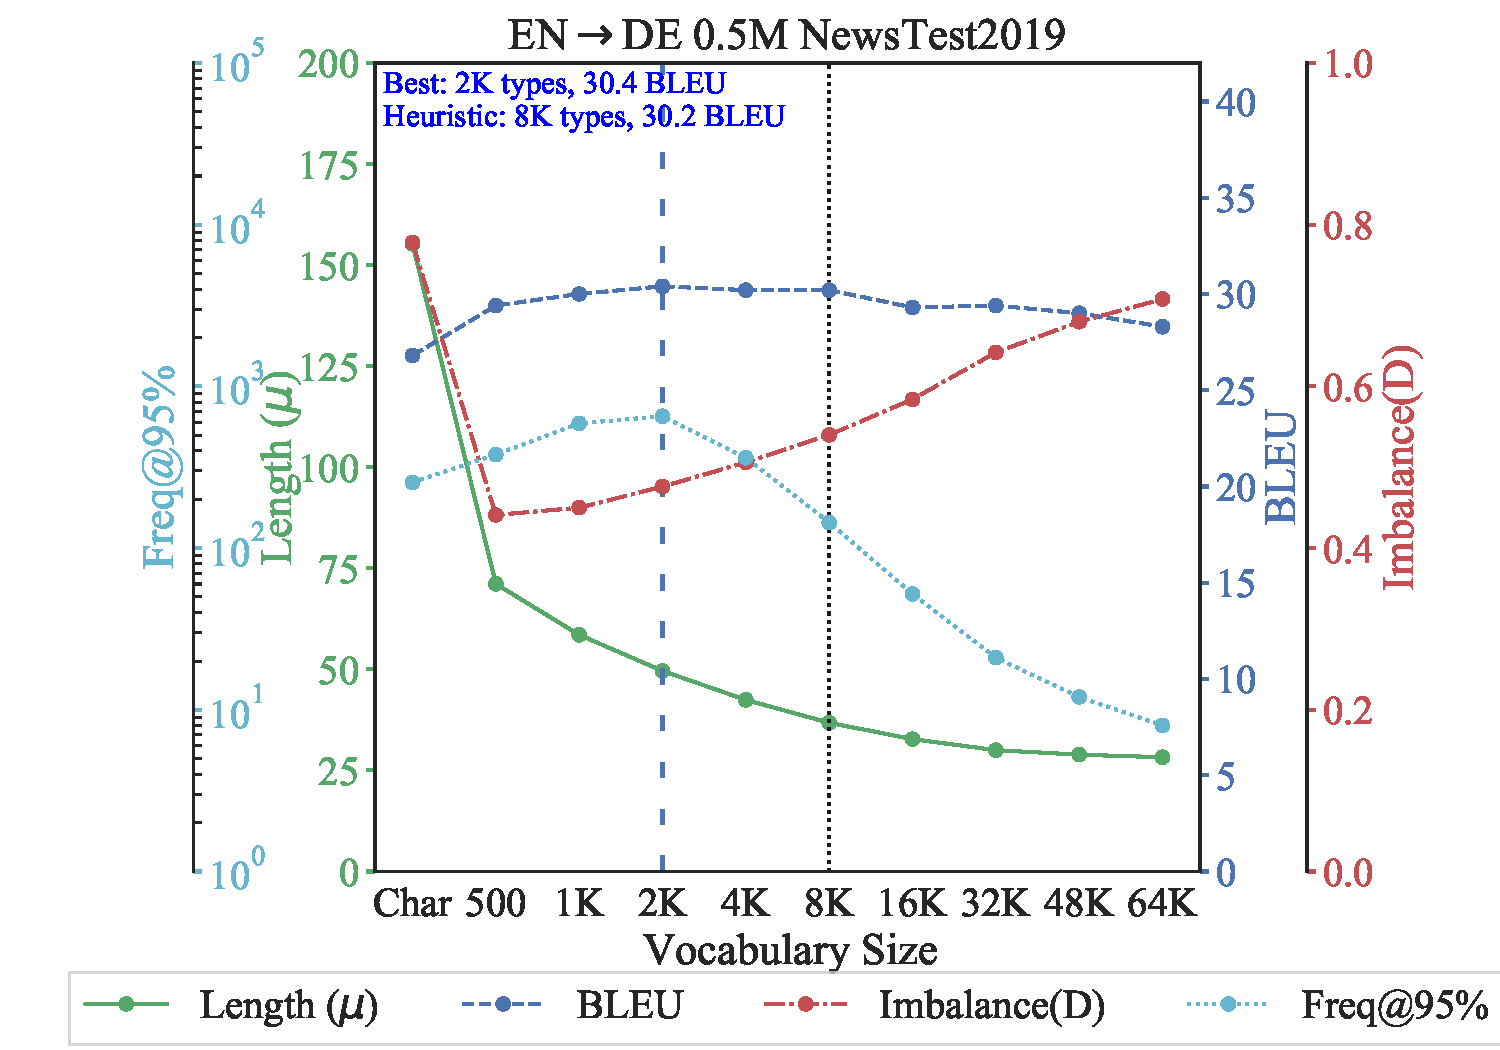
\includegraphics[width=0.99\linewidth,trim={5.1cm 1.32cm 1.4cm 0},clip]{4axv-test-ende-0.5m.pdf}
  %\caption{1c}
  %\label{fig:sfig2}
\end{subfigure}

\caption[Visualization of sequence length, class imbalance, frequency of $95^{th}$ percentile class, and test set BLEU.]{Visualization of sequence length ($\mu$) (lower is better), class imbalance (D) (lower is better), frequency of $95^{th}$ percentile class ($F_{95\%}$) (higher is better; plotted in logarithmic scale), and test set BLEU (higher is better) on all language pairs and training data sizes.
%DE$\leftrightarrow$EN of 1M resembles resembles DE$\leftrightarrow$EN of 0.5M and is provided in Appendix~\ref{sec:appendix} along with visualizations on validation sets.
The vocabulary sizes that achieved highest BLEU are indicated with dashed vertical lines, and the vocabulary our heuristic selects is indicated by dotted vertical lines.}
\label{fig:mu-d-freq-bleu}
\end{figure}

\begin{figure}[h!t]
\ContinuedFloat
\centering

\begin{subfigure}{\textwidth}
  \centering
  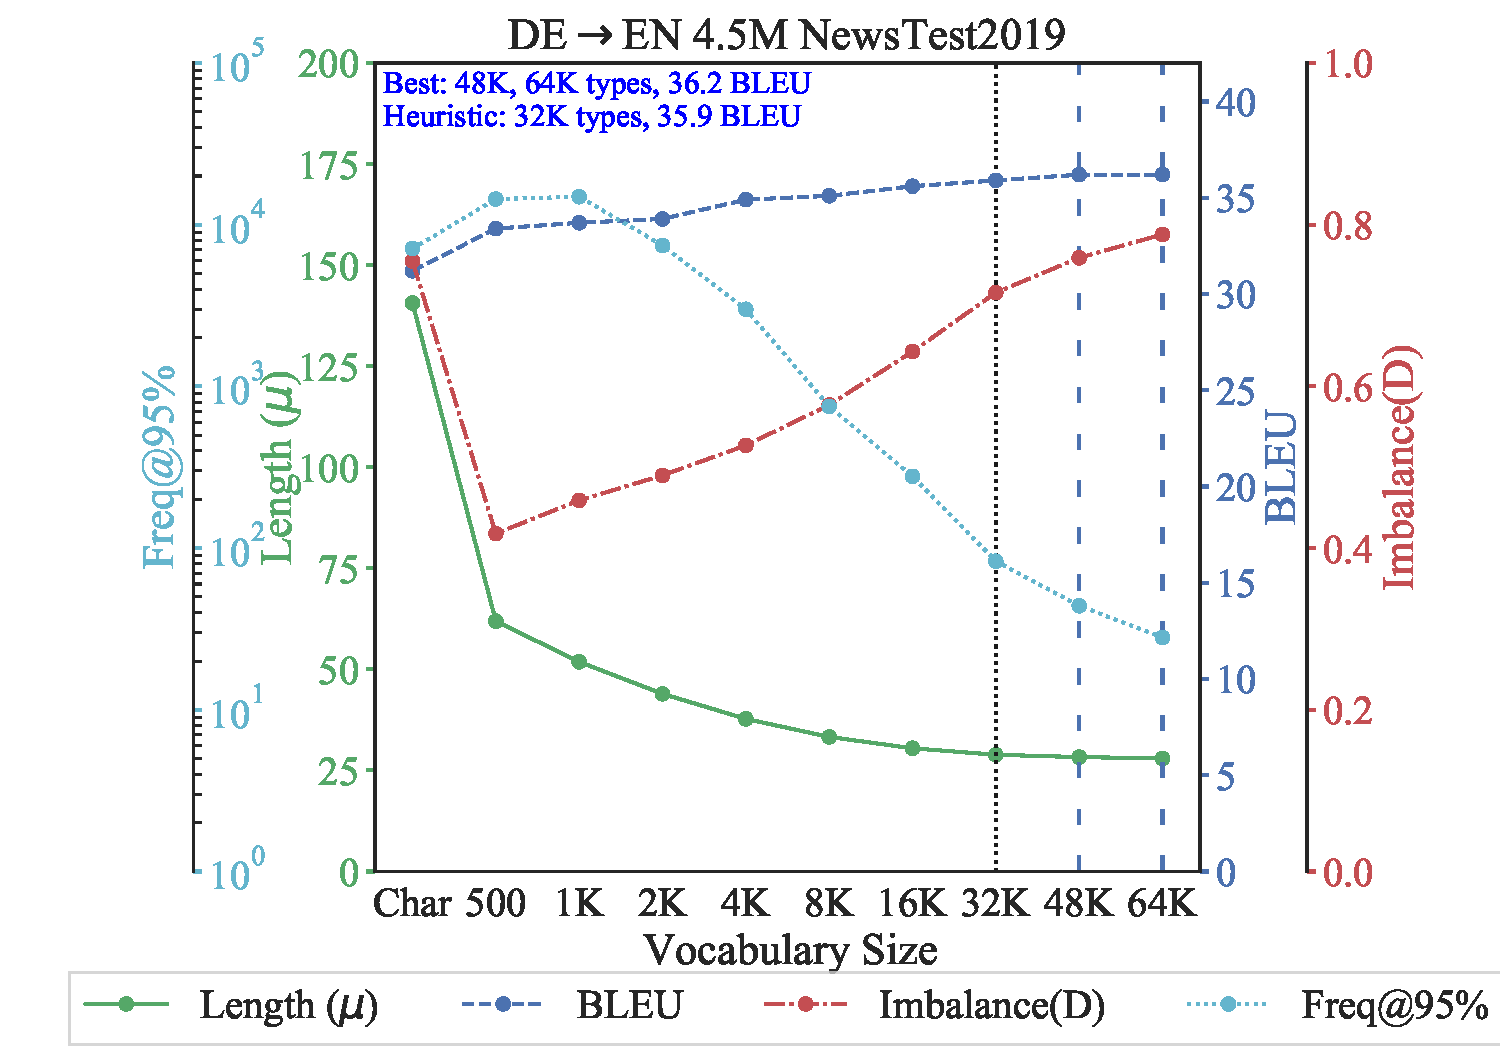
\includegraphics[width=0.7\linewidth,trim={1.4cm 0 0.2cm 16.45cm},clip]{4axv-test-deen-4.5m.pdf}
\end{subfigure}

\vspace{2mm}

\begin{subfigure}{.45\textwidth}
  \centering
  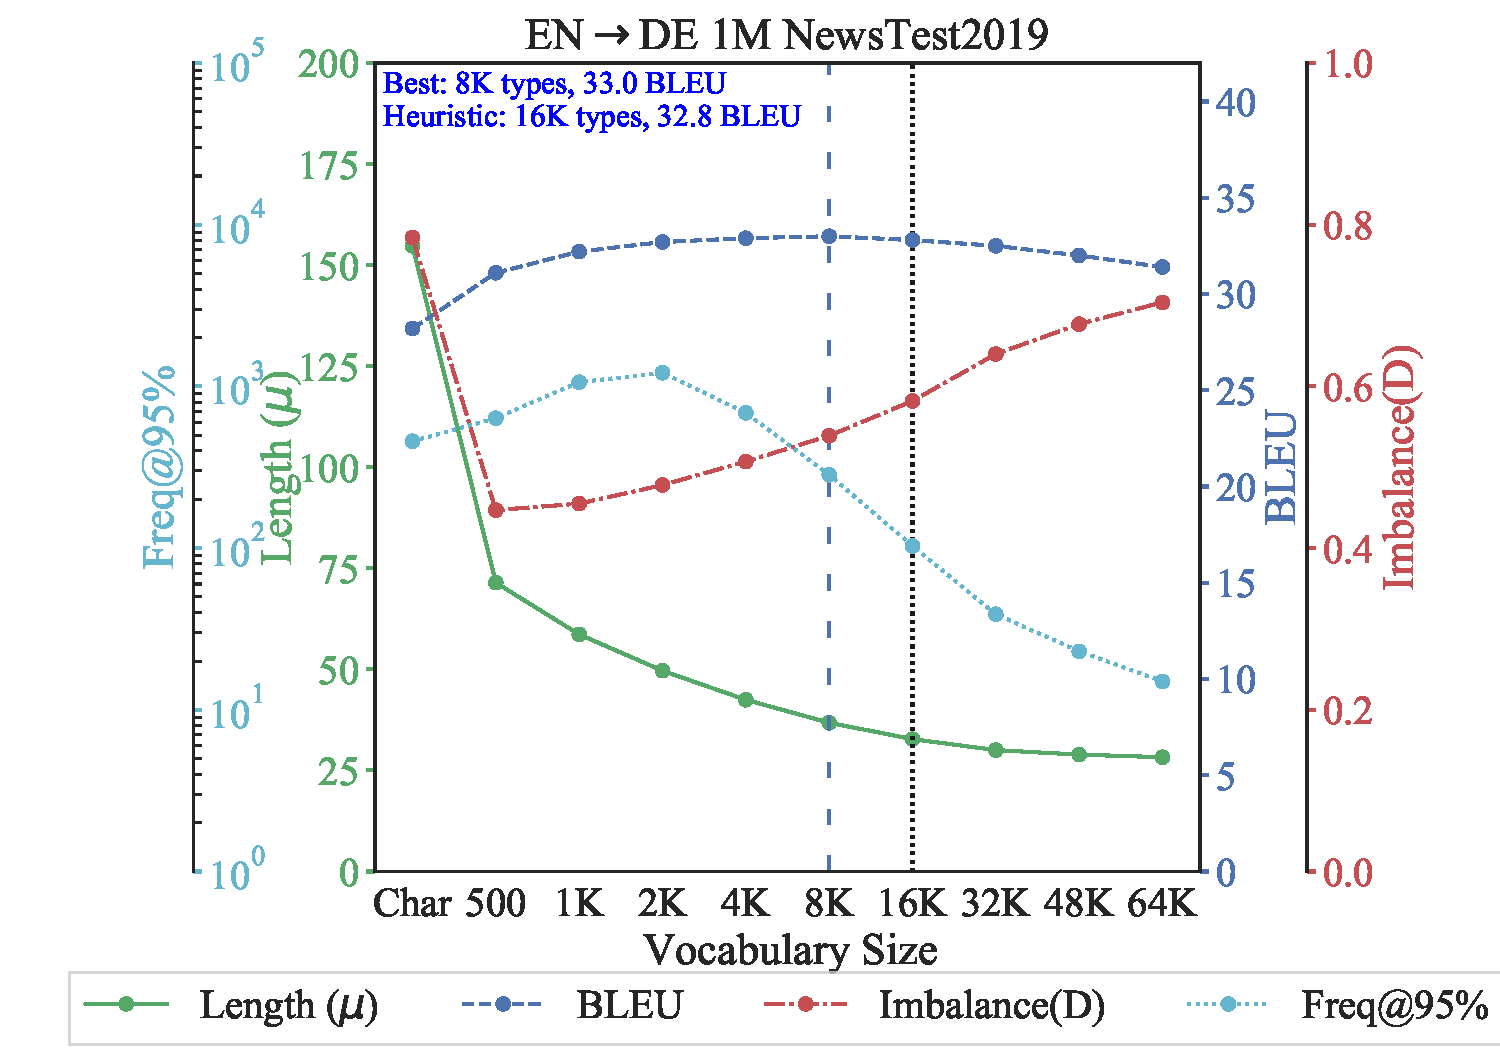
\includegraphics[width=0.99\linewidth,trim={2.4cm 1.32cm 4.1cm 0},clip]{4axv-test-ende-1m.pdf}
 % \caption{1c}
  %\label{fig:sfig2}
\end{subfigure}
\begin{subfigure}{.45\textwidth}
  \centering
  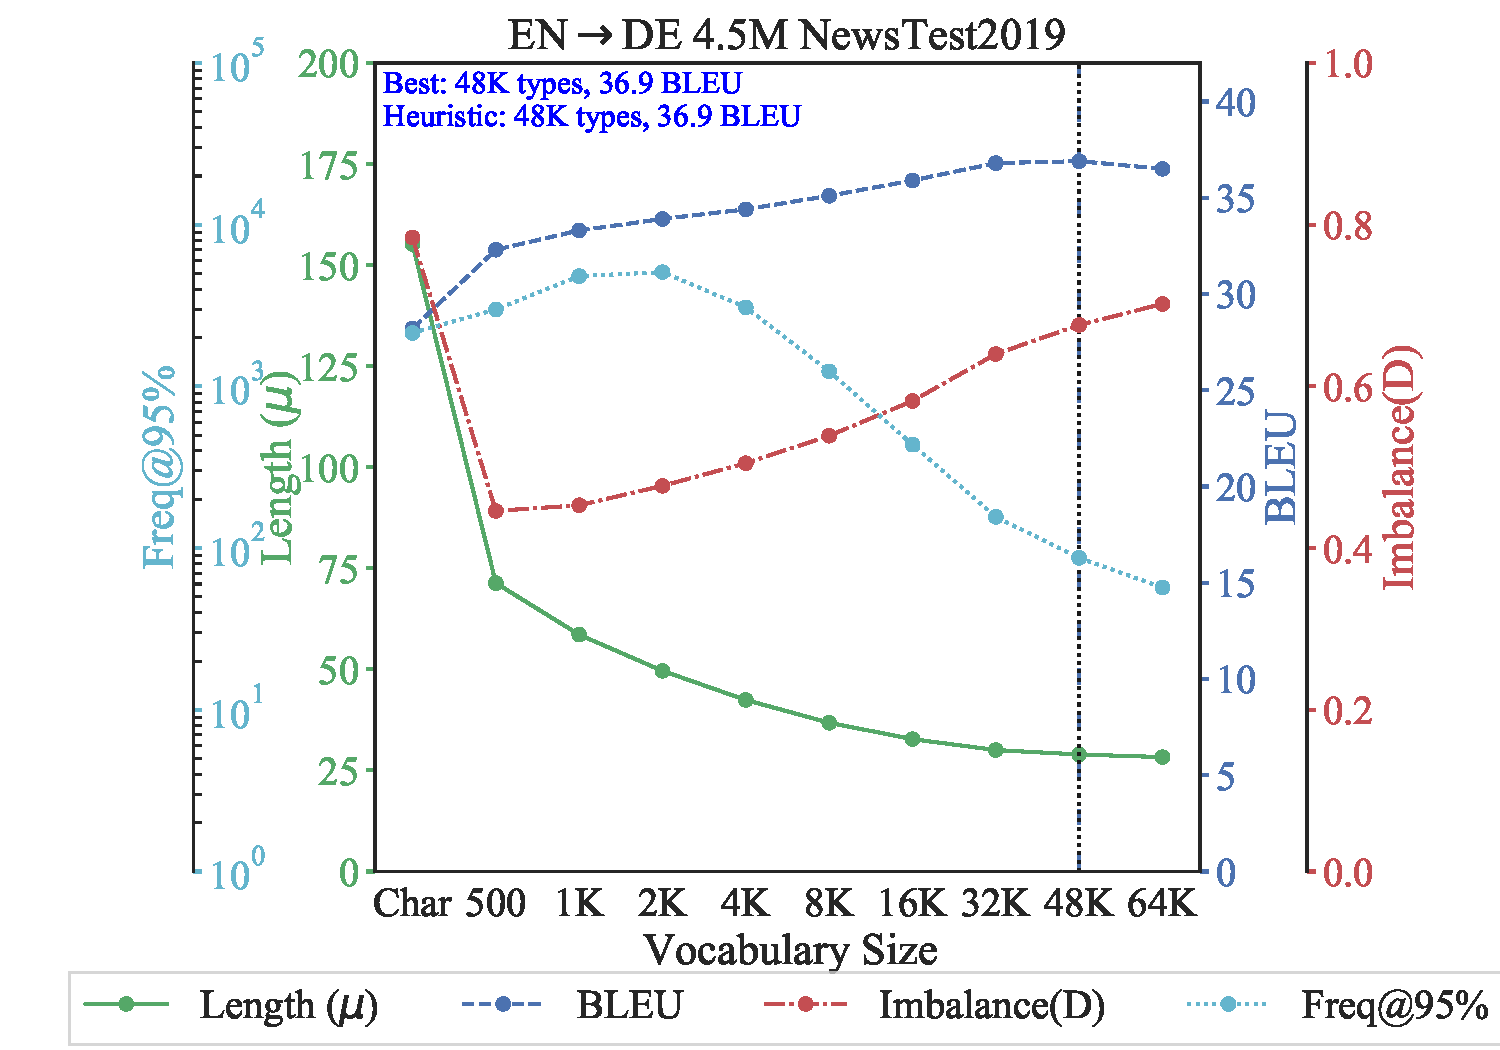
\includegraphics[width=0.99\linewidth,trim={5.1cm 1.32cm 1.4cm 0},clip]{4axv-test-ende-4.5m.pdf}
 % \caption{1c}
  %\label{fig:sfig2}
\end{subfigure}


\begin{subfigure}{.45\textwidth}
  \centering
  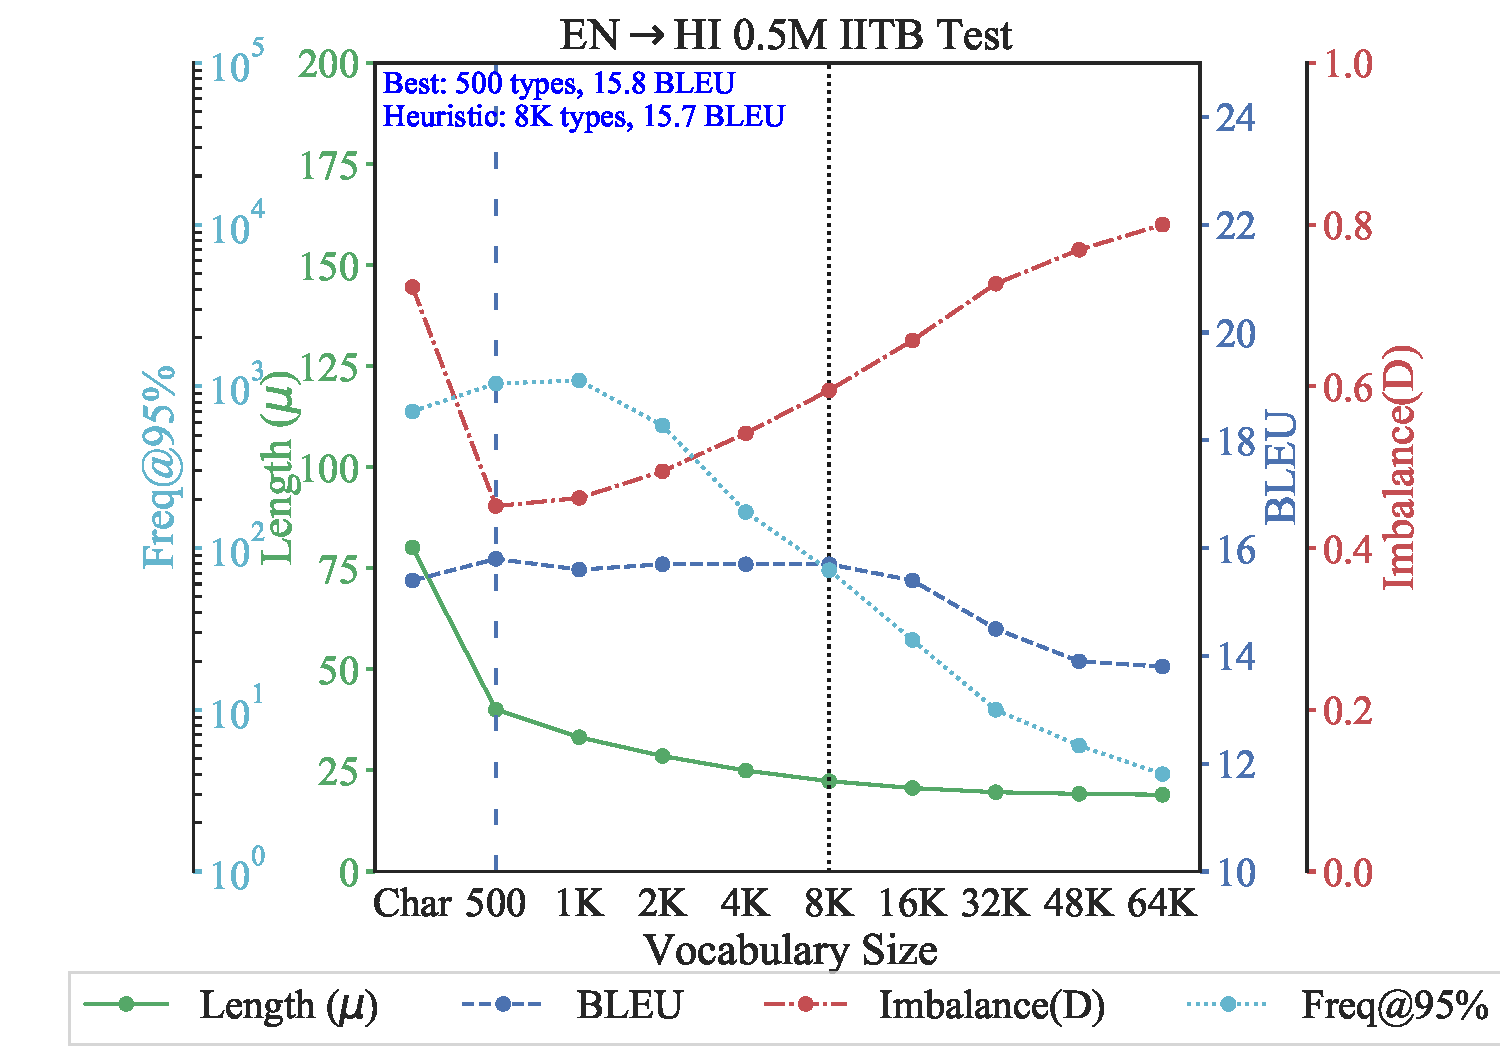
\includegraphics[width=0.99\linewidth,trim={2.4cm 1.32cm 4.1cm 0},clip]{4axv-test-enhi-0.5m.pdf}
 % \caption{1a}
  %\label{fig:sfig1}
\end{subfigure}
\begin{subfigure}{.45\textwidth}
  \centering
  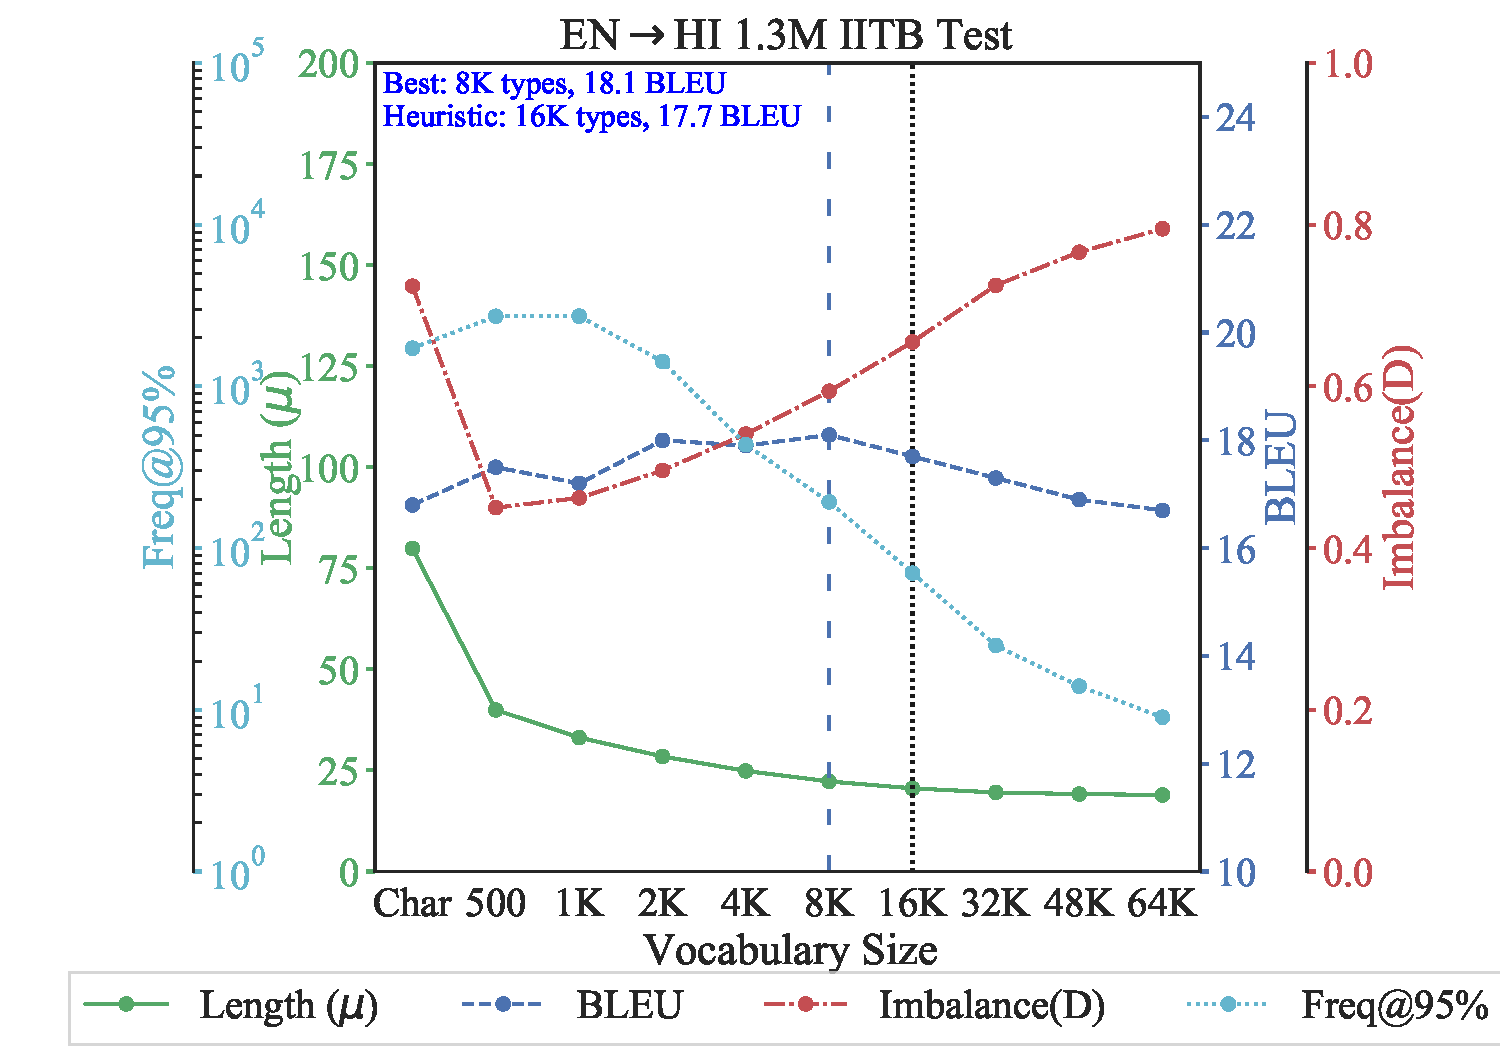
\includegraphics[width=0.99\linewidth,trim={5.1cm 1.32cm 1.4cm 0},clip]{4axv-test-enhi-1.3m.pdf}
  %\caption{1c}
  %\label{fig:sfig2}
\end{subfigure}

\begin{subfigure}{.54\textwidth}
  \centering
  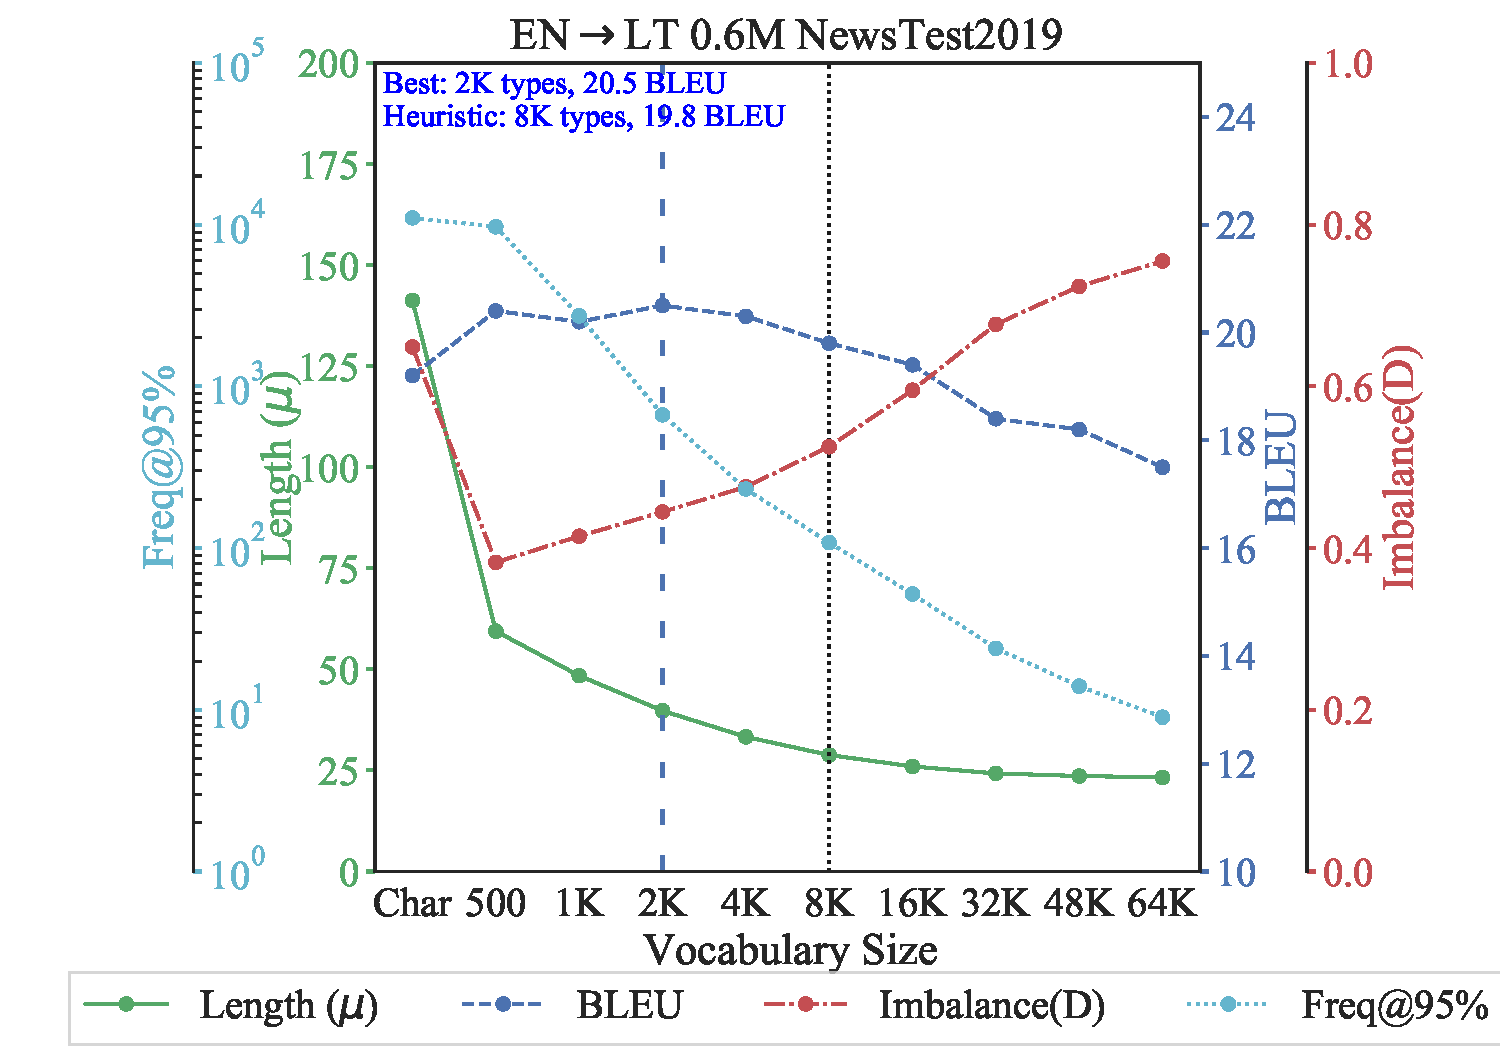
\includegraphics[width=0.99\linewidth,trim={2.4cm 1.32cm 1.4cm 0},clip]{4axv-test-enlt-0.6m.pdf}
  %\caption{1c}
  %\label{fig:sfig2}
\end{subfigure}

\caption{Continuation of Figure~\ref{fig:mu-d-freq-bleu} (see previous page for caption)}
\label{fig:mu-d-freq-bleu-continued}
\end{figure}

BLEU scores are often lower at larger vocabulary sizes---where $\mu$ is (favorably) low but $D$ is (unfavorably) high (Figure~\ref{fig:mu-d-freq-bleu}). This calls for a further investigation that is discussed in the following section.

\section{Measuring Classifier Bias Due to Imbalance}
\label{sec:class-bias}

In a typical classification setting with imbalanced classes, the classifier learns an undesired bias based on frequencies. 

A balanced class distribution debiases in this regard, leading to improvement in the precision of frequent classes as well as recall of infrequent classes.
However, BLEU focuses only on the \textit{precision} of classes; except for adding a global brevity penalty, it is ignorant of the poor recall of infrequent classes. 

Therefore, the BLEU scores shown in Figures~\ref{fig:bleu-deen}, \ref{fig:bleu-ende} and \ref{fig:bleu-enhilt} capture only a part of the improvements and biases. 
In this section, we perform a detailed analysis of the impact of class balancing by considering both precision \textit{and} recall of classes. 

We accomplish this in two stages:
First, we define a method to measure the bias of the model for classes based on their frequencies.
Second, we track the bias in relation to vocabulary size and class imbalance, and report DE$\rightarrow$EN, as it has many data points.

\subsection{Frequency Based Bias}
We measure frequency bias using the Pearson correlation coefficient, $\rho$, between class rank and class performance, while for performance measures we use precision and recall.
Classes are ranked based on descending order of frequencies in the training data, encoded with the same encoding schemes used for reported NMT experiments.
With this setup, the class with rank 1, say $F_1$, is the one with the highest frequency, rank 2 is the next highest, and so on.
More generally, $F_c$ is an index in the class rank list which has an inverse relation to class frequencies.

Following our definitions in Section~\ref{ch:background-sec:eval}, we compute precision ($P_c$) and recall ($R_c$) for each class $c$.
The Pearson correlation coefficients between class rank and precision ($\rho_{F, P}$), and class rank and recall ($\rho_{F, R})$ are reported in Figure \ref{fig:corr-deen-test}.
In datasets where $D$ is high, the performance of classifier correlates with class rank. Such correlations are undesired for a classifier.


\subsection{Analysis of Class Frequency Bias}
An ideal classifier is one that does not discriminate classes based on their frequencies, i.e., one that exhibits no correlation between $\rho_{F, P}$, and$\rho_{F, R}$.  
However, we see in Figure~\ref{fig:corr-deen-test} that:
\begin{enumerate}
    \itemsep0em
    \item $\rho_{F, P}$ is positive when the dataset has high $D$; i.e. if the class rank increases (frequency decreases), precision increases in relation to it.
    This indicates that frequent classes have relatively less precision than infrequent classes.
    The bias is strongly positive on smaller datasets such as 30K DE$\rightarrow$EN, which gradually diminishes if the training data size is increased or a vocabulary setting is chosen to reduce $D$.
    \item $\rho_{F, R}$ is negative, i.e., if the class rank increases, recall decreases in relation to it. 
    This is an indication that infrequent classes have relatively lower recall than frequent classes.
\end{enumerate}
Figure~\ref{fig:corr-deen-test} shows a trend that frequency based bias measured by correlation coefficient is lower in settings that have lower $D$.
However, since $D$ is non-zero, there still exists non-zero correlation between recall and class rank ($\rho_{F, R}$), indicating the poorer recall of low-frequency classes.

%%%%%%%%%%%%%%%%%%%%%%%%%%%%%%%%%%%%%%%%%%%%%%%%%%%%%%%%%%%%%%%%%%%%%%%%%%%%
\section{Conclusion}
\label{sec:conclusion}
Envisioning NMT as a multi-class classifier with an autoregressor helps in analyzing its weaknesses.
Our analysis provides an explanation of \textit{why} text generation using BPE vocabulary is more effective compared to word and character vocabularies, and \textit{why} certain BPE hyperparameters are better than others.
We show that the number of BPE merges is not an arbitrary hyperparameter, and that it can be tuned to address the class imbalance and sequence length problems. 
Our recommendation for Transformer NMT is to \textit{use the largest possible BPE vocabulary, such that at least 95\% of classes have 100 or more examples in training}.
Even though certain BPE vocabulary sizes indirectly reduce the class imbalance, they do not completely eliminate it.
The class distributions after applying BPE contain sufficient imbalance for inducing the frequency based bias, especially affecting the recall of rare classes. 
Hence, more effort in the future is needed to directly address the Zipfian imbalance.

%\section*{Acknowledgments}
%This research is based upon work supported in part by the Office of the Director of National Intelligence (ODNI), Intelligence Advanced Research Projects Activity (IARPA), via contract \# FA8650-17-C-9116, and by research sponsored by Air Force Research Laboratory (AFRL) under agreement number FA8750-19-1-1000. The views and conclusions contained herein are those of the authors and should not be interpreted as necessarily representing the official policies, either expressed or implied, of ODNI, IARPA, Air Force Laboratory, DARPA, or the U.S. Government. The U.S. Government is authorized to reproduce and distribute reprints for governmental purposes notwithstanding any copyright annotation therein.

\chapter{Minority Categories and Affirmative Action}
\label{ch:affirmative-action}

\setlength{\epigraphwidth}{5.6in} 
\epigraph{\textit{``The test of our progress is not whether we add more to the abundance of those who have much; it is whether we provide enough for those who have too little."} --- Franklin D. Roosevelt, 1937.}

%ML applications are being deployed in human society; they are automating many services historically handled by humans.

Human society is imbalanced in various forms, e.g., people are categorized based on their gender, age, race, religious affiliation, and nationality, which result in imbalanced classes.
This imbalance lead to the formation of majority and minority groups in the society.
A lot of policies are made to address it.
In this chapter, we consider the policies and strategies aimed to address the societal imbalance as an opportunity to study and translate them into machine learning setting.
When policies are decided based on the support or benefit of majority number of citizens, the minority groups have little say in such system and are usually corned. 
In machine learning, certain metrics such as Accuracy that do not account for imbalance lead to overlooking of minority classes. 
The historic negative discrimination towards minority classes affect the opportunities of disadvantaged groups and their fair competitiveness in the present times.
To combat this historical negative discrimination, several governing bodies either encourage or mandate positive discrimination towards minority categories.
These positive discrimination -- called Affirmative Action (AA) \cite{affirmative-action} -- are a set of policies and strategies installed by government aiming to boost the career and educational opportunities for minority groups.  
Since the opportunities in most competitive settings are of zero-sum game, boosting the minority groups implies that the majority groups are deliberately put to a disadvantage.
Similar to how the negative discrimination is problematic, even the positive discrimination can also be problematic and it is controversial, especially since it violates the notion of equality. 
However, some social scientists argue that there is some merit to the positive discrimination if the intention is to reverse the imbalance that already exists, especially if it can be accomplished without significantly hurting the majority categories.
%\footnote{``\textit{The test of our progress is not whether we add more to the abundance of those who have much; it is whether we provide enough for those who have too little.}" -- Franklin D. Roosevelt, 1937. \url{https://www.fdrlibrary.org/fdr}; accessed: June 2021.}
AA methods are broadly classified into two kinds: (1) quota-based in which certain percentile of opportunities are reserved for disadvantaged groups, and (2) preference-based in which disadvantaged groups are given a special preference in the selection process.

Since ML techniques deal with imbalanced categories in which some categories are at a disadvantage, we wonder if teaching machines the affirmative actions is a good idea.
We rephrase it more concretely as the following questions: 
\begin{enumerate}
    \item When AA is required in ML?
    \item What are the ethical implications of having AA in ML?
    \item How to quantify the impact of AA in ML?
    \item What AA approaches are most effective in ML?
\end{enumerate}

The above questions are addressed briefly in the following subsections:

\section{When AA is required in ML?}
ML techniques perform well on, and often favorably biased towards, the majority classes. 
If the performance on majority classes is more important than the minority classes, then AA methods are not needed.
In some extreme cases of such scenarios, the ML itself may not be needed, as one could  ignore minority classes and simply assign majority category label to \textit{all} examples.
More often in practice, the classifier performance on minority classes is at least as important, if not more, as that of majority classes.
Even in such scenarios, if ML techniques are fair and just for all categories, then AA is not needed. 
However, an extensive body of work confirms that in the presence of imbalanced categories, ML techniques are often unfavorably biased towards minority categories.
Hence AA (i.e. positive discrimination) is required to counter act the frequency-based biases and achieve better performance across all classes and especially the minority classes. 

\section{Ethical implications of having AA in ML}
TODO:

No free-lunch theorem.

\section{How to quantify the impact of AA in ML?}
Evaluation metrics are a key component of ML pipeline.
To assess the impact of AA, we need evaluation metrics that offer performance breakdown to the granularity of individual categories.
Some metrics, e.g. \textit{accuracy},  offer only the system's overall performance and not its breakdown to individual categories, and hence they are less useful.
By using metrics that break down scores to each category, we can directly compare the difference in performance between the baseline non-AA versus AA methods for all categories individually.
AA method is effective if it has a significant performance improvement for crucial categories without significantly hurting the performance of other less-important categories. 
Although we do not aim for reducing the performance on less-important classes, in practice, due to the zero-sum game nature of the setting, there may be negative impact on some categories.

\section{What AA approaches are effective in ML?}
Efforts towards addressing imbalance in the context of ML classifiers are as follows:
\textit{Imbalanced learning} are some of the techniques that favor minority classes by counter acting the inherent frequency based biased of ML modeling.
We survey, and report in detail in Chapter ~\ref{ch:imb-learning}.
The recent trend is to simply add more training examples; although the imbalance ratio retains,  due to the \textit{`law diminishing returns'}, the minority classes are often more benefited more than majority classes from adding more training examples.
  % <-- not sure where this goes

\chapter{Evaluation: Rare Words are Important Too}
\label{ch:eval-metrics}

\setlength{\epigraphwidth}{5.6in} 
\epigraph{\textit{``The test of our progress is not whether we add more to the abundance of those who have much; it is whether we provide enough for those who have too little."} --- Franklin D. Roosevelt, 1937}



Model-based metrics for evaluating machine translation such as BLEURT \cite{sellam-etal-2020-bleurt}, ESIM \cite{mathur-etal-2019-ESIM}, and YiSi \cite{lo-2019-yisi} have recently attracted attention due to their superior correlation with human judgments \cite{WMT19-metrics-proceedings}. However, \bleu~\cite{papineni-etal-2002-bleu} remains  the most widely used corpus-level MT metric. It correlates reasonably well with human judgments, and moreover is easy to understand and cheap to calculate, requiring only reference translations in the target language. By contrast, model-based metrics require tuning on thousands of examples of human evaluation for every new target language or domain \cite{sellam-etal-2020-bleurt}. Model-based metric scores are also opaque and can hide undesirable biases, as can be seen in Table~\ref{tab:bleurt-bias}.


\begin{table}[ht]
    \centering
    %\footnotesize
    \begin{tabular}{l l l }
Reference: & \multicolumn{2}{l}{You must be a doctor.} \\
Hypothesis: & \multicolumn{2}{l}{$\rule{1cm}{0.15mm}$ must be a doctor.} \\
    % & You &	~0.990 \\
    & He	&-0.735 \\
    & Alexandra & -0.888 \\
    & Alexander & -0.975 \\
    & Joe & -0.975 \\
    & Sue & -1.043 \\
    & She & -1.100 \\\hline
Reference:& \multicolumn{2}{l}{It is the greatest country in the world.} \\
Hypothesis:& \multicolumn{2}{l}{$\rule{1cm}{0.15mm}$ is the greatest country in the world.} \\
    %& It	& ~0.957 \\
    & France &	-0.022 \\
    & America	& -0.060 \\
    & Russia &	-0.161 \\
    & China  & -0.166 \\
    & USA    & -0.168 \\
    & India   &	-0.211 \\
    & Canada  & -0.309 
    \end{tabular}
    \caption{A demonstration of BLEURT's internal biases; model-free metrics like BLEU would consider each of the errors above to be equally wrong.}
    \label{tab:bleurt-bias}
\end{table}

The source of model-based metrics' (e.g., BLEURT) correlative superiority over model-free metrics (e.g., BLEU) appears to be the former's ability to focus evaluation on \textit{adequacy}, while the latter are overly focused on \textit{fluency}. BLEU and most other generation metrics consider each output \textit{token} equally. Since natural language is dominated by a few high-count types, an MT model that concentrates on getting its \textit{if}s, \textit{and}s and \textit{but}s right will benefit from BLEU in the long run more than one that gets its \textit{xylophone}s, \textit{peripatetic}s, and \textit{defenestrate}s right. Can we derive a metric with the discriminating power of BLEURT that does not share its bias or expense and is as interpretable as BLEU? 

As it turns out, the metric may already exist and be in common use. Information extraction and other areas concerned with classification have long used both \textit{micro averaging}, which treats each token equally, and \textit{macro averaging}, which instead treats each \textit{type} equally, when evaluating. The latter in particular is useful when seeking to avoid results dominated by overly frequent types. In this chapter, we take a classification-based approach to evaluating machine translation by considering word type imbalance into account. We obtain an easy-to-calculate metric that focuses on adequacy as much as BLEURT but does not have the expensive overhead, opacity, or bias of model-based methods. 


Our contributions are as follows:
We consider MT as a classification task, and thus admit \maf1 as a legitimate approach to evaluation~(Section ~\ref{sec:mt-as-cls}). 
We show that \maf1 is competitive with other popular methods at tracking human judgments in translation (Section~\ref{sec:wmt-metrics}). 
We offer an additional justification of \maf1 as a performance indicator on adequacy-focused downstream tasks such as cross-lingual information retrieval (Section \ref{sec:clir}). 
Finally, we demonstrate that \maf1 is just as good as the expensive BLEURT at discriminating between structurally different MT approaches in a way \bleu\ cannot, especially regarding the adequacy of generated text (Section \ref{sec:unmt}).


\section{MT Evaluation: Micro and Macro Metrics}
\label{sec:mt-as-cls}
In section~\ref{sec:classifier-nlg}, we have provided a high-level view of NMT. 
Specifically, we view NMT as a multi-class classifier that operates on representations from an autoregressor.
We may thus consider classifier-based evaluation metrics for MT.  

As per the notation and definitions in Section~\ref{ch:background-sec:eval}, consider a test corpus, $T = \{ (x^{(i)}, h^{(i)}, y^{(i)}) | i = 1,2,3 ... N \}$ where $x^{(i)}$, $h^{(i)}$, and $y^{(i)}$ are source, system hypothesis, and reference translation, respectively. Let $x = \{x^{(i)} \forall i\}$ and similar for $h$ and $y$.  Let $V_h, V_y, V_{h\cap y},$ and $V$ be the vocabulary of $h$, the vocabulary of $y$, $V_h \cap V_y$, and $V_h \cup V_y$, respectively.
Following our definitions in Section~\ref{ch:background-sec:eval}), we compute $F_\beta$ measure ($F_{\beta;c}$) for each unigram type $c \in V_{h \cap y}$:\footnote{We consider $F_{\beta;c}$ for $c \not\in V_{h \cap y}$ to be 0.}

The \textit{macro-average} consolidates individual performance by averaging by type, while the \textit{micro-average} averages by token:
\begin{align*}
\maf\beta &= \frac{\sum_{c \in V} F_{\beta;c}} {|V|}\\
\mif\beta &= \frac{\sum_{c\in V} freq(c) \times F_{\beta;c}} {\sum_{c'\in V} f(c')}
\end{align*}
\noindent where $freq(c) = \textsc{Refs}(c)+k$ for smoothing factor $k$.\footnote{We use $k=1$. When $k \rightarrow \infty, \space \mif\beta \rightarrow \maf\beta. $} We scale $\maf\beta$ and $\mif\beta$ values to percentile, similar to \bleu, for the sake of easier readability.

\section{Justification for \texorpdfstring{\maf1}{MacroF1}}
\label{sec:justific}

In the following sections, we verify and justify the utility of \maf1 while also offering a comparison with popular alternatives such as \mif1, \bleu, \chrf{1}, and BLEURT.\footnote{\bleu\ and \chrf1 scores reported in this work are computed with \textsc{SacreBleu}; see the Appendix for details.
BLEURT scores are from the \textit{base} model \citep{sellam-etal-2020-bleurt}. We consider two varieties of averaging to obtain a corpus-level metric from the segment-level BLEURT: mean and median of segment-level scores per corpus.}
We use Kendall's rank correlation coefficient, $\tau$, to compute the association between metrics and human judgments.
Correlations with p-values smaller than $\alpha=0.05$ are considered to be statistically significant.

\begin{figure}[ht]
    \centering
    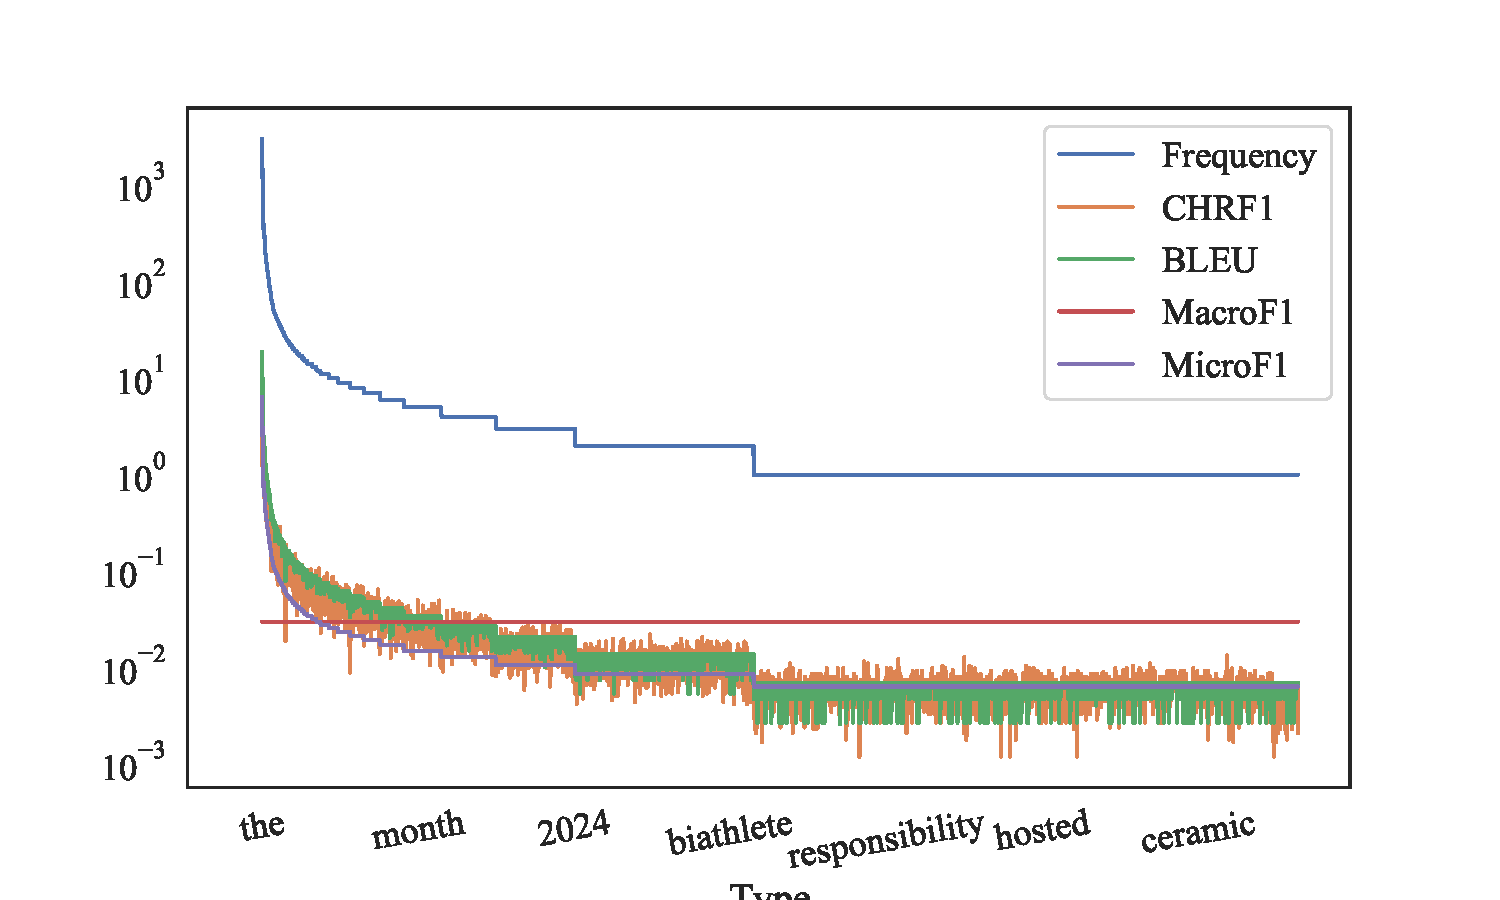
\includegraphics[width=\textwidth,trim={0mm 5mm 0mm 0mm},clip]{img/macroavg/bleu-chrf-macro-micro-swapin-lenmatch.pdf}
    \caption{MT metrics and their weights assigned to word types.
    Statistics are from WMT 2019 German-English NewsTest reference corpus.
    While \maf1{} treat each type equally, all others treat each token equally. }
    \label{fig:bleu-damage}
\end{figure}

\subsection{Data-to-Text: WebNLG}
\label{sec:webnlg}


\begin{table}[ht]
%    \footnotesize
    \centering
    \begin{tabular}{lrr}
Name & Fluency \& Grammar & Semantics \\ \hline\hline
\bleu\  & \insig.444 & \insig.500 \\
\chrf1 & \insig.278    & .778   \\
\maf1  & \insig.222    & .722   \\
\mif1  & \insig.333    & .611   \\ \hline
\blrtmn & \insig.444   & .833   \\
\blrtmd & .611  & .667   \\
\end{tabular}
    \caption{WebNLG data-to-text task: Kendall's $\tau$ between system-level MT metric scores and human judgments.
    Fluency and grammar are correlated identically by all metrics.
    Values that are \textit{not} significant at $\alpha=0.05$ are indicated by \insig{}.}
    \label{tab:webnlg-kendall}
\end{table}


We use the 2017 WebNLG Challenge dataset \cite{gardent2017webNLG-corpus, shimorina2018webnlg-human-eval}\footnote{\url{https://gitlab.com/webnlg/webnlg-human-evaluation}} to analyze the differences between micro- and macro- averaging. 
WebNLG is a task of generating English text for sets of triples extracted from DBPedia.
Human annotations are available for a sample of 223 records each from nine NLG systems.
The human judgments provided have three linguistic aspects---fluency, grammar, and semantics\footnote{Fluency and grammar, which are elicited with nearly identical directions \cite{gardent2017webNLG-corpus}, are identically correlated.}---which enable us to perform a fine-grained analysis of our metrics.
We compute Kendall's $\tau$ between metrics and human judgments, which are reported in Table~\ref{tab:webnlg-kendall}.

As seen in Table~\ref{tab:webnlg-kendall}, the metrics exhibit much variance in agreements with human judgments. %Fluency and grammar display same correlations and hence are com  
For instance, \blrtmd\ is the best indicator of fluency and grammar, however \blrtmn\ is best on semantics. 
BLEURT, being a \textit{model-based} measure that is directly trained on human judgments, scores relatively higher than others.
Considering the model-free metrics, \chrf1 does well on semantics but poorly on fluency and grammar compared to \bleu.
Not surprisingly, both \mif1 and \maf1, which rely solely on unigrams, are poor indicators of fluency and grammar compared to \bleu, however \maf1 is clearly a better indicator of semantics than \bleu. 
The discrepancy between \mif1 and \maf1 regarding their agreement with fluency, grammar, and semantics is expected: micro-averaging pays more attention to function words (as they are frequent types) that contribute to fluency and grammar whereas macro-averaging pays relatively more attention to the content words that contribute to semantic adequacy. 

The takeaway from this analysis is as follows: \maf1 is a strong indicator of semantic adequacy, however, it is a poor indicator of fluency. We recommend using either \maf1 or \chrf1 when semantic adequacy and not fluency is a desired goal.

\subsection{Machine Translation: WMT Metrics}
\label{sec:wmt-metrics}

\begin{table*}[ht!]
    %\footnotesize
    %\small
    \centering
    
\begin{tabular}{r r l r r r r r }
Year & Pairs  & & $\star$\bleu\ & \bleu\ & \maf1 & \mif1 & \chrf1 \\ \hline\hline
\multirow{3}{*}{ 2019 } 
    & \multirow{3}{*}{18}
     & Mean   & .751 & .771 & .821 & .818 & .841  \\ 
   & & Median & .782 & .752 & .844 & .844 & .875  \\
   & & Wins   &     3 &     3 &  \textbf{6}    &     3 &   5 \\ \hline
\multirow{3}{*}{ 2018 } 
  & \multirow{3}{*}{14}
   & Mean   & .858 & .857 & .875 & .873 & .902  \\ 
  & & Median & .868 & .868 & .901 & .879 & .919  \\
  & & Wins    &  1  &  2 & 3 &  2 &  \textbf{6}\\ \hline  
\multirow{3}{*}{ 2017 }
   & \multirow{3}{*}{13}
    & Mean   & .752 & .713 & .714 & .742 & .804 \\  
  & & Median & .758 & .733 & .735 & .728 & .791 \\
  & & Wins   & 5 & 4 & 2 & 2 & \textbf{6} \\
\end{tabular}   
\caption[WMT 2017--19 Metrics task: Mean and median Kendall's $\tau$ between MT metrics and human judgments.]{WMT 2017--19 Metrics task: Mean and median Kendall's $\tau$ between MT metrics and human judgments.
Correlations that are not significant at $\alpha=0.05$ are excluded from the calculation of mean, and median, and wins.
See Appendix Tables \ref{tab:wmt19-kendall}, \ref{tab:wmt18-kendall}, and \ref{tab:wmt17-kendall} for full details.
$\star$\bleu\ is pre-computed scores available in the metrics packages.
In 2018 and 2019, both \maf1 and \mif1 outperform \bleu, \maf1 outperforms \mif1.
\chrf1 has strongest mean and median agreements across the years.
Judging based on the number of wins, \maf1 has steady progress over the years, and outperforms others in 2019.
}
\label{tab:wmt-summary}
\end{table*}

In this section, we verify how well the metrics agree with human judgments using Workshop on Machine Translation (WMT) metrics task datasets for 2017--2019~\cite{WMT17-metrics,WMT18-metrics,WMT19-metrics-proceedings}.\footnote{\url{http://www.statmt.org/wmt19/metrics-task.html}}
We first compute scores from each MT metric, and then calculate the correlation $\tau$ with human judgments.

As there are many language pairs and translation directions in each year, we report only the mean and median of $\tau$, and number of wins per metric for each year in Table \ref{tab:wmt-summary}.
We have excluded BLEURT from comparison in this section since the BLEURT models are fine-tuned on the same datasets on which we are evaluating the other methods.\footnote{\url{https://github.com/google-research/bleurt}}
\chrf1 has the strongest mean and median agreement with human judgments across the years.
In 2018 and 2019, both \maf1 and \mif1 mean and median agreements outperform \bleu\, whereas in 2017 \bleu\ was better than \maf1 and \mif1.


As seen in Section~\ref{sec:webnlg}, \maf1 weighs towards semantics whereas \mif1 and \bleu\ weigh towards fluency and grammar.
This indicates that recent MT systems are mostly fluent, and adequacy is the key discriminating factor amongst them.
\bleu\ served well in the early era of statistical MT when fluency was a harder objective. 
Recent advancements in neural MT models such as Transformers \cite{vaswani-2017-attention} produce fluent outputs, and have brought us to an era where semantic adequacy is the focus.


% save it for the slides
%We envision that the methods such as \maf1 that emphasize the long tail be more successful in the future years, and this vision is inline with \citet{steedman-2008-last}:
%One day, either because of the demise of Moore’slaw, or simply because we have done all the easy stuff, the Long Tail will come back to haunt us.
%\textit{``One day, ... simply because we have done all the easy stuff, the Long Tail will come back to haunt us.''}


%\section{Agreement with WMT Human Judgments}
%\label{sec:apphuman}

Tables \ref{tab:wmt19-kendall}, \ref{tab:wmt18-kendall}, and \ref{tab:wmt17-kendall} provide $\tau$ between MT metrics and human judgments on WMT Metrics task 2017--2019. 
$\star$\bleu\ is based on pre-computed scores in WMT metrics package, whereas \bleu\ is based on our recalculation using \textsc{SacreBleu}. 
Values marked with \insig are not significant at $\alpha=0.05$, and hence corresponding rows are excluded from the calculation of mean, median, and standard deviation.

Since \maf1 is the only metric that does not achieve statistical significance in the WMT 2019 EN-ZH setting, we carefully inspected it.
Human scores for this setting are obtained without looking at the references by bilingual speakers \cite{WMT19-metrics-proceedings}, but the ZH references are found to have a large number of bracketed EN phrases, especially proper nouns that are rare types.
When the text inside these brackets is not generated by an MT system, \maf1 naturally penalizes heavily due to the poor recall.
Since other metrics assign lower importance to poor recall of such rare types, they achieve relatively better correlation to human scores than \maf1. 
However, since the $\tau$ values for EN-ZH are relatively lower than the other language pairs, we conclude that poor correlation of \maf1 in EN-ZH is due to poor quality references.
Some settings did not achieve statistical significance due to a smaller sample set as there were fewer MT systems submitted, e.g. 2017 CS-EN.

\begin{table}[ht!]
    %\footnotesize
\small 
\parbox{.48\linewidth}{
\centering
\begin{tabular}{l @{\hspace{1mm}} r @{\hspace{1mm}} r @{\hspace{1mm}} r @{\hspace{1mm}} r @{\hspace{1mm}} r}
 & $\star$\bleu & \bleu & \maf1 & \mif1 & \chrf1 \\ \hline \hline
DE-CS & .855 & .745 & .964 & .917 & \textbf{.982}  \\
DE-EN & .571 & .655 & .723 & .695 & \textbf{.742} \\
DE-FR & .782 & .881 & \textbf{.927} & .844 & .915 \\
EN-CS & .709 & \textbf{.954} & .927 & .927 & .908  \\
EN-DE & .540 & .752 & .741 & .773 & \textbf{.824} \\
EN-FI & .879 & .818 & .879 & .848 & \textbf{.923}  \\
EN-GU & .709 & .709 & .600 & \textbf{.734} & .709  \\
EN-KK & .491 & .527 & \textbf{.685} & .636 & .661  \\
EN-LT & .879 & .848 & \textbf{.970} & .939 & .881 \\
EN-RU & .870 & .848 & \textbf{.939} & .879 & .930  \\
FI-EN & .788 & .809 & \textbf{.909} & .901  & .875 \\
FR-DE & \textbf{.822} & .733 & .733 & .764  & .815 \\
GU-EN & .782 & .709 & .855 & .891 & \textbf{.945}  \\
KK-EN & \textbf{.891} & .844 & .796 & .844 & .881 \\
LT-EN & .818 & \textbf{.855} & .844 & \textbf{.855}  & .833 \\
RU-EN & .692 & .729 & .714 & \textbf{.780} & .757 \\
ZH-EN & .695 & .695 & \textbf{.752} & .676 & .715 \\ \hline
Median & .782 & .752 & .844 & .844 & .875\\
Mean & .751 & .771 & .821 & .818 & .841  \\
SD & .124 & .101 & .112 & .093 & .095  \\ \hline
EN-ZH & \textbf{.606} & \textbf{.606} & \insig.424 & .595 & .594 \\ \hline
Wins & 3 & 3 & 6 & 3 & 5 
\end{tabular} 
\caption{ WMT19 Metrics task: Kendall's $\tau$ between metrics and human judgments.}
\label{tab:wmt19-kendall}
}
\hfill
%\end{table}
%\vspace{2px}
%\begin{table}[ht]
    %\footnotesize
\parbox{.48\linewidth}{
%    \centering
\begin{tabular}{l @{\hspace{1mm}} r @{\hspace{1mm}} r @{\hspace{1mm}} r @{\hspace{1mm}} r @{\hspace{1mm}} r}
 & $\star$\bleu & \bleu & \maf1 & \mif1 & \chrf1 \\ \hline \hline
DE-EN & .828 & .845 & .917 & .883 & \textbf{.919}  \\
EN-DE & .778 & .750 & \textbf{.850} & .783 & .848  \\
EN-ET & .868 & .868 & .934 & .906 & \textbf{.949}  \\
EN-FI & .901 & .848 & .901 & .879 & \textbf{.945}  \\
EN-RU & .889 & .889 & \textbf{.944} & .889 & .930  \\
EN-ZH & .736 & .729 & .685 & \textbf{.833} & .827 \\
ET-EN & .884 & .900 & .884 & .878 & \textbf{.904}  \\
FI-EN & .944 & .944 & .889 & .915 & \textbf{.957}  \\
RU-EN & .786 & .786 & \textbf{.929} & .857 & .869 \\
ZH-EN & .824 & \textbf{.872} & .738 & .780 & .820  \\ 
EN-CS & \textbf{1.000} & \textbf{1.000} & .949 & \textbf{1.000} & .949  \\ \hline

Median & .868 & .868 & .901 & .879 & .919  \\
Mean   & .858 & .857 & .875 & .873 & .902  \\
SD     & .077 & .080 & .087 & .062 & .052  \\ \hline

TR-EN & \insig.200 & \insig.738 & \insig.400 & \insig.316 & \insig.632 \\
EN-TR & \insig.571 & \insig.400 & .837 & \insig.571 & \textbf{.849}  \\
CS-EN & \insig.800 & \insig.800 & \insig.600 & \insig.800 & \insig.738 \\ \hline
Wins &  1  &  2 & 3 &  2 & 6
\end{tabular}
\caption{ WMT18 Metrics task: Kendall's $\tau$ between metrics and human judgments.}
\label{tab:wmt18-kendall}
}
\end{table}


%\vspace{2px}
\begin{table}[ht]
    %\footnotesize
    \centering
\begin{tabular}{l @{\hspace{1.5mm}} r @{\hspace{1.5mm}} r @{\hspace{1.5mm}} r @{\hspace{1.5mm}} r @{\hspace{1.5mm}} r}
 & $\star$\bleu & \bleu & \maf1 & \mif1 & \chrf1 \\ \hline \hline
DE-EN & .564 & .564 & .734 & .661 & \textbf{.744}  \\
EN-CS & .758 & .751 & .767 & .758 & \textbf{.878} \\
EN-DE & .714 & \textbf{.767} & .562 & .593 & .720  \\
EN-FI & .667 & .697 & .769 & .718 & \textbf{.782} \\
EN-RU & .556 & .556 & \textbf{.778} & .648 & .669  \\
EN-ZH & \textbf{.911} & \textbf{.911} & .600 & .854 & .899 \\
LV-EN & \textbf{.905} & .714 & \textbf{.905} & \textbf{.905} & \textbf{.905}  \\
RU-EN & .778 & .611 & .611 & .722 & \textbf{.800}  \\
TR-EN & \textbf{.911} & .778 & .674 & .733 & .907  \\
ZH-EN & .758 & \textbf{.780} & .736 & .824 & .732  \\ \hline
Median & .758 & .733 & .735 & .728 & .791 \\
Mean & .752 & .713 & .714 & .742 & .804  \\
SD & .132 & .110 & .103 & .097 & .088  \\ \hline
FI-EN & \textbf{.867} & \textbf{.867} & \insig.733 & \textbf{.867} & \textbf{.867} \\
EN-TR & \textbf{.857} & .714 & \insig.571 & .643 & .849 \\
CS-EN & \insig1.000 & \insig1.000 & \insig.667 & \insig.667 & \insig.913 \\  \hline
Wins & 5 & 4 & 2 & 2 & 6
\end{tabular} 
\caption{ WMT17 Metrics task: Kendall's $\tau$ between metrics and human judgments.}
\label{tab:wmt17-kendall}
\end{table}



\subsection{Downstream Task: Cross-Lingual Information Retrieval}
\label{sec:clir}
In this section, we determine correlation between MT metrics and  downstream cross-lingual information retrieval (CLIR) tasks.
CLIR is a kind of information retrieval (IR) task in which documents in one language are retrieved given queries in another~\cite{grefenstette2012CLIR}. 
A practical solution to CLIR is to translate source documents into the query language using an MT model, then use a monolingual IR system to match queries with translated documents. 
Correlation between MT and IR metrics is accomplished in the following steps: 
\begin{enumerate}[noitemsep,topsep=0pt]
 \item Build a set of MT models and measure their performance using MT metrics.
 \item Using each MT model in the set, translate all source documents to the target language, build an IR model, and measure IR performance on translated documents.
 \item For each MT metric, find the correlation between the set of MT scores and their corresponding set of IR scores.
 The MT metric that has a stronger correlation with the IR metric(s) is more useful than the ones with weaker correlations.
\item Repeat the above steps on many languages to verify the generalizability of findings.
\end{enumerate}


An essential resource for this analysis is a dataset with human annotations for computing MT and IR performances.
We conduct experiments on two datasets: firstly, on data from the 2020 workshop on \textit{Cross-Language Search and Summarization of Text and Speech} (CLSSTS) \cite{zavorin-etal-2020-corpora}, and secondly, on data originally from Europarl, prepared by \citet{lignos-etal-2019-MT-IR} (Europarl).

\subsubsection{CLSSTS Datasets}
\label{sec:material}

\begin{table*}[ht]
    %\footnotesize
    \small 
    \begin{tabular}{l l l r r r r r r }
 & Domain & IR Score & \bleu\ & \maf1 & \mif1 & \chrf1 & {\footnotesize \blrtmn} & {\footnotesize \blrtmd} \\\hline\hline

\multirow{4}{*}{LT-EN} 
& \multirow{2}{*}{In} 
  & AQWV & .429 & \insig.363 & \textbf{.508} & \insig.385 & .451  & .420 \\
& & MAP  & .495  & .429      & \textbf{.575} & .451       & .473  & .486 \\
& \multirow{2}{*}{In+Ext}
   & AQWV & \insig.345 & \textbf{.527} & .491  & .491 & .491 & .477 \\
&  & MAP  & \insig.273 & \insig\textbf{.455} & \insig.418 & \insig.418 & \insig.418 & \insig.404 \\\hline
\multirow{4}{*}{PS-EN}
  & \multirow{2}{*}{In} 
    & AQWV  & .559 & \textbf{.653} & .574 & .581 & .584 & .581  \\
  & & MAP   & .493 & \textbf{.632} & .487 & .494 & .558 & .554 \\
  & \multirow{2}{*}{In+Ext}
    & AQWV   & .589 & \textbf{.682} & .593 & .583 & .581 & .571 \\
  & & MAP    & .519 & \textbf{.637} & .523 & .482 & .536 & .526 \\\hline
\multirow{4}{*}{BG-EN}
 & \multirow{2}{*}{In} 
    & AQWV   & \insig.455 & \textbf{.550}   & .527  & \insig.382 & \insig.418  & .418 \\ 
 &  & MAP    &  .491      &  \textbf{.661}  & .564  &  .491       & .527       & .527 \\ 
 & \multirow{2}{*}{In+ext}
    & AQWV   & \insig.257 & \textbf{.500}       & \insig.330 & \insig.404 & \insig.367 & \insig.367 \\
 &  & MAP   & \insig.183 & \insig\textbf{.426} & \insig.257 & \insig.330 & \insig.294 & \insig.294 
\end{tabular} 
\caption{CLSSTS CLIR task: Kendall's $\tau$ between IR and MT metrics under study.
The rows with Domain=In are where MT and IR scores are computed on the same set of documents, whereas Domain=In+Ext are where IR scores are computed on a larger set of documents that is a superset of segments on which MT scores are computed.
\textbf{Bold} values are the best correlations achieved in a row-wise setting; values with \insig~ are \textit{not} significant at $\alpha=0.05$.}
\label{tab:material-kendall}
\end{table*}


CLSSTS datasets contain queries in English~(EN), and documents in many source languages along with their human translations, as well as query-document relevance judgments. 
We use three source languages: Lithuanian~(LT), Pashto~(PS), and Bulgarian~(BG).
The performance of this CLIR task is evaluated using two IR measures: Actual Query Weighted Value (AQWV) and Mean Average Precision (MAP).
AQWV\footnote{\href{https://www.nist.gov/system/files/documents/2017/10/26/aqwv\_derivation.pdf}{https://www.nist.gov/system/files/documents-/2017/10/26/aqwv\_derivation.pdf}} is derived from Actual Term Weighted Value (ATWV) metric \cite{wegmann2013ATWV}. 
We use a single CLIR system \cite{boschee-etal-2019-saral} with the same IR settings for all MT models in the set, and measure Kendall's $\tau$ between MT and IR measures.
The results, in Table~\ref{tab:material-kendall}, show that \maf1 is the strongest indicator of CLIR downstream task performance in five out of six settings.
AQWV and MAP have a similar trend in agreement to the MT metrics.
\chrf1 and BLEURT, which are strong contenders when generated text is directly evaluated by humans, do not indicate CLIR task performance as well as \maf1, as CLIR tasks require faithful meaning equivalence across the language boundary, and human translators can mistake fluent output for proper translations \cite{callison-burch-etal-2007-meta}. 


\subsubsection{Europarl Datasets}
\label{sec:lignos-etal}

\begin{table}[ht]
    %\footnotesize
    \centering
    %\setlength{\tabcolsep}{10pt}
\begin{tabular}{l r r r r r r}
 & \bleu\ & \maf1 & \mif1 & \chrf1 & \blrtmn & \blrtmd \\ \hline\hline
\multirow{1}{*}{ CS-EN } 
 & .850 & .867 & .850 & .850 & \textbf{.900} & .867 \\ 
\multirow{1}{*}{ DE-EN } 
  & .900 & .900 & .900 & .912 & \textbf{.917} & .900 \\
\end{tabular}  
\caption{Europarl CLIR task: Kendall's $\tau$ between MT metrics and RBO. All correlations are significant at $\alpha=0.05$.}
\label{tab:lignos-mtir-kendall} 
\end{table}


We perform a similar analysis to Section \ref{sec:material} but on another cross-lingual task set up by \citet{lignos-etal-2019-MT-IR} for Czech $\rightarrow$ English (CS-EN) and German $\rightarrow$ English (DE-EN), using publicly available data from the Europarl v7 corpus~\cite{koehn2005europarl}. 
This task differs from the CLSSTS task (Section \ref{sec:material}) in several ways.
Firstly, MT metrics are computed on test sets from the news domain, whereas IR metrics are from the Europarl domain. The domains are thus intentionally mismatched between MT and IR tests.
Secondly, since there are no queries specifically created for the Europarl domain, GOV2 TREC topics 701–850 are used as domain-relevant English queries.
And lastly, since there are no query-document relevance human judgments for the chosen query and document sets, the documents retrieved by BM25~\cite{jones2000probabilistic} on the English set for each query are treated as relevant documents for computing the performance of the CS-EN and DE-EN CLIR setup. 
As a result, IR metrics that rely on boolean query-document relevance judgments as ground truth are less informative, and we use Rank-Based Overlap (RBO; $p=0.98$) \cite{webber2010RBO} as our IR metric.

We perform our analysis on the same experiments as \citet{lignos-etal-2019-MT-IR}.\footnote{\url{https://github.com/ConstantineLignos/mt-clir-emnlp-2019}}
NMT models for CS-EN and DE-EN translation are trained using a convolutional NMT architecture \cite{gehring2017CNNMT} implemented in the FAIRSeq~\cite{ott-etal-2019-fairseq} toolkit.
For each of CS-EN and DE-EN, a total of 16 NMT models that are based on different quantities of training data and BPE hyperparameter values are used.
The results in Table~\ref{tab:lignos-mtir-kendall} show that BLEURT has the highest correlation in both cases.
Apart from the trained \blrtmd\ metric, \maf1 scores higher than the others on CS-EN, and is competitive on CS-EN. \maf1 is not the metric with the highest IR task correlation in this setting, unlike in Section \ref{sec:material}, however it is competitive with \bleu\ and \chrf1, and thus a safe choice as a downstream task performance indicator. 


\section{Spotting Differences Between Supervised and Unsupervised NMT}
\label{sec:unmt}

Unsupervised neural machine translation (UNMT) systems trained on massive monolingual data without parallel corpora have made significant progress recently \cite{Artetxe-2018-unmt-iclr,Lample-2018-unmt-iclr,lample-etal-2018-phrase-unmt,conneau-NIPS2019-xlm,Song-2019-MASS,liu-etal-2020-multilingual-denoising}. 
In some cases, UNMT yields a \bleu\ score that is comparable with strong\footnote{though not, generally, the strongest} supervised neural machine translation (SNMT) systems. In this section we leverage \maf1 to investigate differences in the translations from UNMT and SNMT systems that have similar \bleu.

We compare UNMT and SNMT for English $\leftrightarrow$ German (EN-DE, DE-EN), English $\leftrightarrow$ French (EN-FR, FR-EN), and English $\leftrightarrow$ Romanian (EN-RO, RO-EN).
All our UNMT models are based on XLM \citep{conneau-NIPS2019-xlm}, pretrained by \citet{XLM-UNMT-Models20}. 
We choose SNMT models with similar \bleu\ on common test sets by either selecting from systems submitted to previous WMT News Translation shared tasks~\cite{bojar-etal-2014-findings,bojar-etal-2016-findings} or by building such systems.\footnote{We were unable to find EN-DE and DE-EN systems with comparable \bleu\ in WMT submissions so we built standard Transformer-base~\cite{vaswani-2017-attention} models for these using appropriate quantity of training data to reach the desired \bleu\ performance. We report EN-RO results with diacritic removed to match the output of UNMT.} Specific SNMT models chosen are in Table~\ref{tab:unmt_vs_snmt2}. 
The UNMT models follow XLM's standard architecture and are trained with 5 million monolingual sentences for each language using a vocabulary size of 60,000. 
% using code base from \citet{rtg-xt20}
We train SNMT models for EN$\leftrightarrow$DE and select models with the most similar (or a slightly lower) BLEU as their UNMT counterparts on newstest2019. The DE-EN model selected is trained with 1 million sentences of parallel data and a vocabulary size of 64,000, and the EN-DE model selected is trained with 250,000 sentences of parallel data and a vocabulary size of 48,000. For EN$\leftrightarrow$FR and EN$\leftrightarrow$RO, we select SNMT models from submitted systems to WMT shared tasks that have similar or slightly lower BLEU scores to corresponding UNMT models, based on \textit{NewsTest2014} for EN$\leftrightarrow$FR and \textit{NewsTest2016} for EN$\leftrightarrow$RO. 

%\subsection{UNMT and SNMT Models}
\begin{table}[ht!]
% \resizebox{\textwidth}{!}{%
\centering
%\footnotesize
\begin{tabular}{l @{\hspace{1.5mm}} r @{\hspace{1.5mm}} r @{\hspace{1.5mm}} l}
Translation & SNMT    & UNMT  &  SNMT Name      \\ \hline \hline
DE-EN NewsTest2019     & 32.7   & 33.9  & \textit{Our Transformer}             \\
EN-DE NewsTest2019     & 24.0   & 24.0  & \textit{Our Transformer}           \\
FR-EN NewsTest2014     & 31.1   & 31.2  & OnlineA.0             \\
EN-FR NewsTest2014     & 25.6   & 27.1  & PROMT-Rule-based.3083 \\
RO-EN NewsTest2016     & 30.8   & 29.6  & Online-A.0            \\
EN-RO NewsTest2016     & 31.2   & 31.0  & uedin-pbmt.4362      \\ 
\end{tabular}%
% }
\caption{ We select SNMT systems such that their \bleu\ scores are approximately the same as the available pretrained UNMT models. \textit{Our Transformer} models are the ones we have trained, which are described in  Chapter~\ref{ch:nlg-imbalance}.} 
\label{tab:unmt_vs_snmt2}
\end{table}


\begin{table*}[ht!]
\centering
\small
\setlength{\tabcolsep}{4pt}
%\footnotesize
\begin{tabular}{l @{\hspace{3mm}} r @{\hspace{1.5mm}} r @{\hspace{1.5mm}}r :  r@{\hspace{1.5mm}}r@{\hspace{1.5mm}}r :
  r@{\hspace{1.5mm}}r@{\hspace{1.5mm}}r : r@{\hspace{1.5mm}} r@{\hspace{1.5mm}} r : r@{\hspace{1.5mm}} r@{\hspace{1.5mm}} r : r @{\hspace{1.5mm}} r@{\hspace{1.5mm}} r}
& \multicolumn{3}{c:}{\bleu} & \multicolumn{3}{c:}{ \maf1 } & \multicolumn{3}{c:}{ \mif1 } & \multicolumn{3}{c:}{ \chrf1 } & \multicolumn{3}{c:}{ \blrtmn } & \multicolumn{3}{c}{ \blrtmd } \\ 
& SN & UN & $\Delta$ & SN & UN & $\Delta$ & SN & UN & $\Delta$ & SN & UN & $\Delta$ & SN & UN & $\Delta$ & SN & UN & $\Delta$ \\ \hline \hline
DE-EN & 32.7 & 33.9 & -1.2 & 38.5 & 33.6 & 4.9 & 58.7 & 57.9 &  0.8 & 59.9 & 58.0 &  1.9 & .211 & -.026 & .24 & .285 & .067 & .22 \\
EN-DE & 24.0 & 24.0 &  0.0 & 24.0 & 23.5 & 0.5 & 47.7 & 48.1 & -0.4 & 53.3 & 52.0 &  1.3 &-.134 & -.204 & .07 &-.112 &-.197 & .09 \\
FR-EN & 31.1 & 31.2 & -0.1 & 41.6 & 33.6 & 8.0 & 60.5 & 58.3 &  2.2 & 59.1 & 57.3 &  1.8 & .182 &  .066 & .17 & .243 & .154 & .09 \\
EN-FR & 25.6 & 27.1 & -1.5 & 31.9 & 27.3 & 4.6 & 53.0 & 52.3 &  0.7 & 56.0 & 57.7 & -1.7 & .104 &  .042 & .06 & .096 & .063 & .03 \\
RO-EN & 30.8 & 29.6 &  1.2 & 40.3 & 33.0 & 7.3 & 59.8 & 56.5 &  3.3 & 58.0 & 54.7 &  3.3 & .004 & -.058 & .06 & .045 & -.004 & .04 \\
EN-RO & 31.2 & 31.0 &  0.2 & 34.6 & 31.0 & 3.6 & 55.4 & 53.4 &  2.0 & 59.3 & 56.7 &  2.6 & .030 & -.046 & .08 & .027 & -.038 & .07 \\
\end{tabular} 

\caption{For each language direction, UNMT (UN) models have similar \bleu\ to SNMT (SN) models, and \chrf1 and \mif1 have small differences. 
However, \maf1 scores differ significantly, consistently in favor of SNMT. Both corpus-level interpretations of BLEURT support the trend reflected by \maf1, but the value differences are difficult to interpret. Credits: Weiqiu You.
}
\label{tab:unmt_vs_snmt}
\end{table*}


 Table~\ref{tab:unmt_vs_snmt} shows performance for these three language pairs using a variety of metrics. Despite comparable scores in \bleu\ and only minor differences in \mif1 and \chrf1, SNMT models have consistently higher \maf1 and BLEURT than the UNMT models for all six translation directions. 
 
 
 Figure~\ref{fig:snmt_vs_unmt}, which is a visualization of \maf1 for SNMT and UNMT models,  shows that UNMT is generally better than SNMT on frequent types, however, SNMT outperforms UNMT on the rest leading to a crossover point in \maf1 curves. 
Since \maf1 assigns relatively higher weights to infrequent types than in \bleu{}, SNMT gains higher \maf1 than UNMT while both have approximately the same \bleu{}, as reported in Table~\ref{tab:unmt_vs_snmt}.

\begin{figure}[ht!]
    \centering
    \begin{subfigure}[b]{0.495\linewidth}
    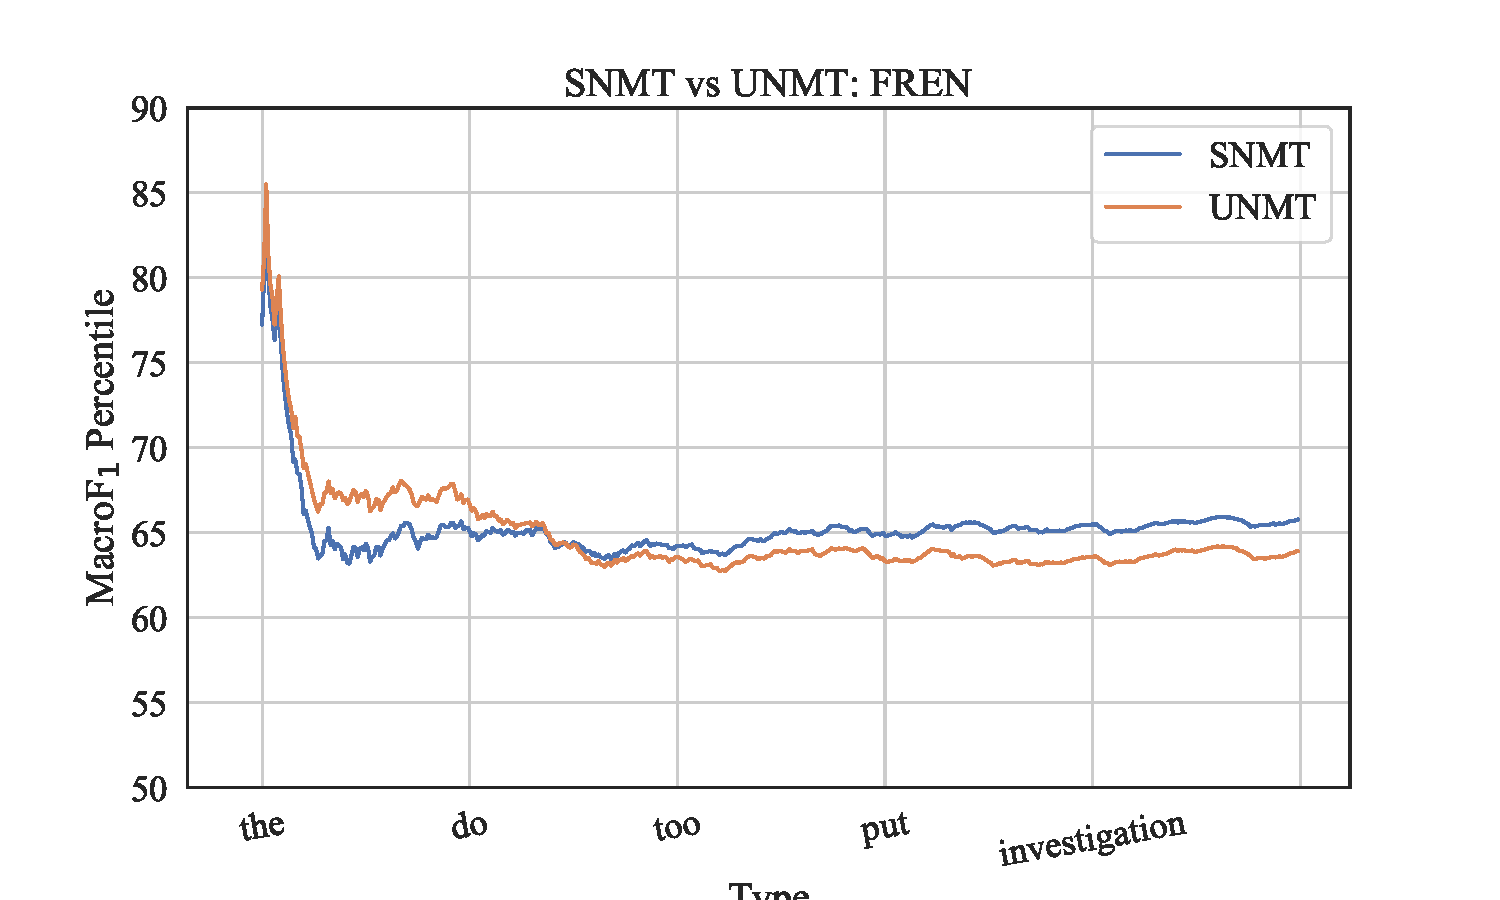
\includegraphics[width=\linewidth,trim={13mm 5mm 25mm 10mm},clip]{macroavg/s_unmt-fren-maf1.pdf}
    \end{subfigure}
    \begin{subfigure}[b]{0.495\linewidth}
    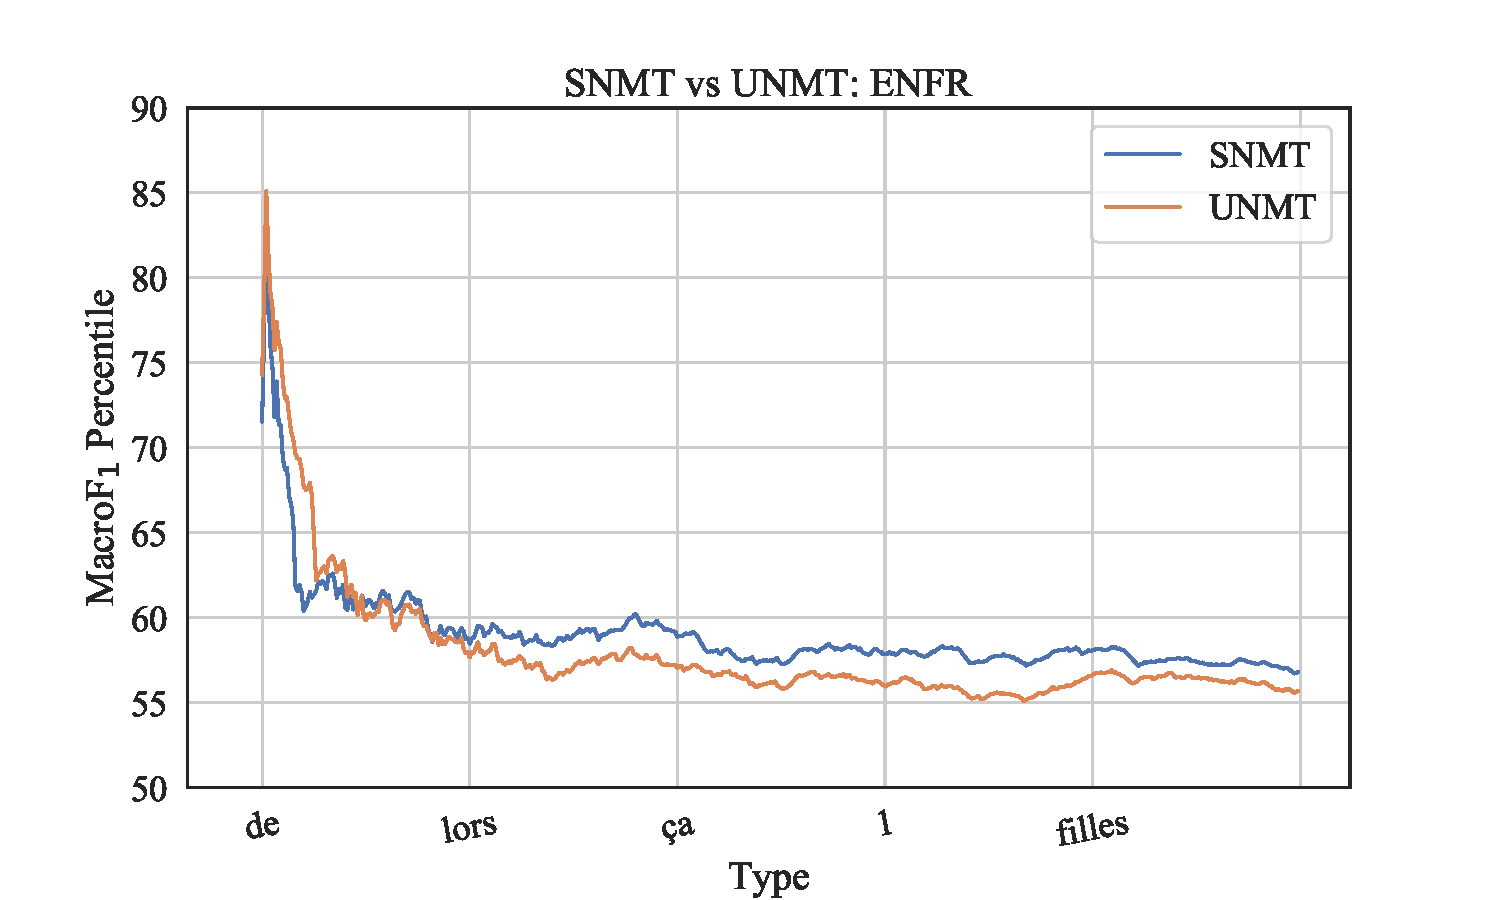
\includegraphics[width=\linewidth,trim={13mm 7mm 25mm 10mm},clip]{macroavg/s_unmt-enfr-maf1.pdf}
    \end{subfigure}
    
    \begin{subfigure}[b]{0.495\linewidth}
    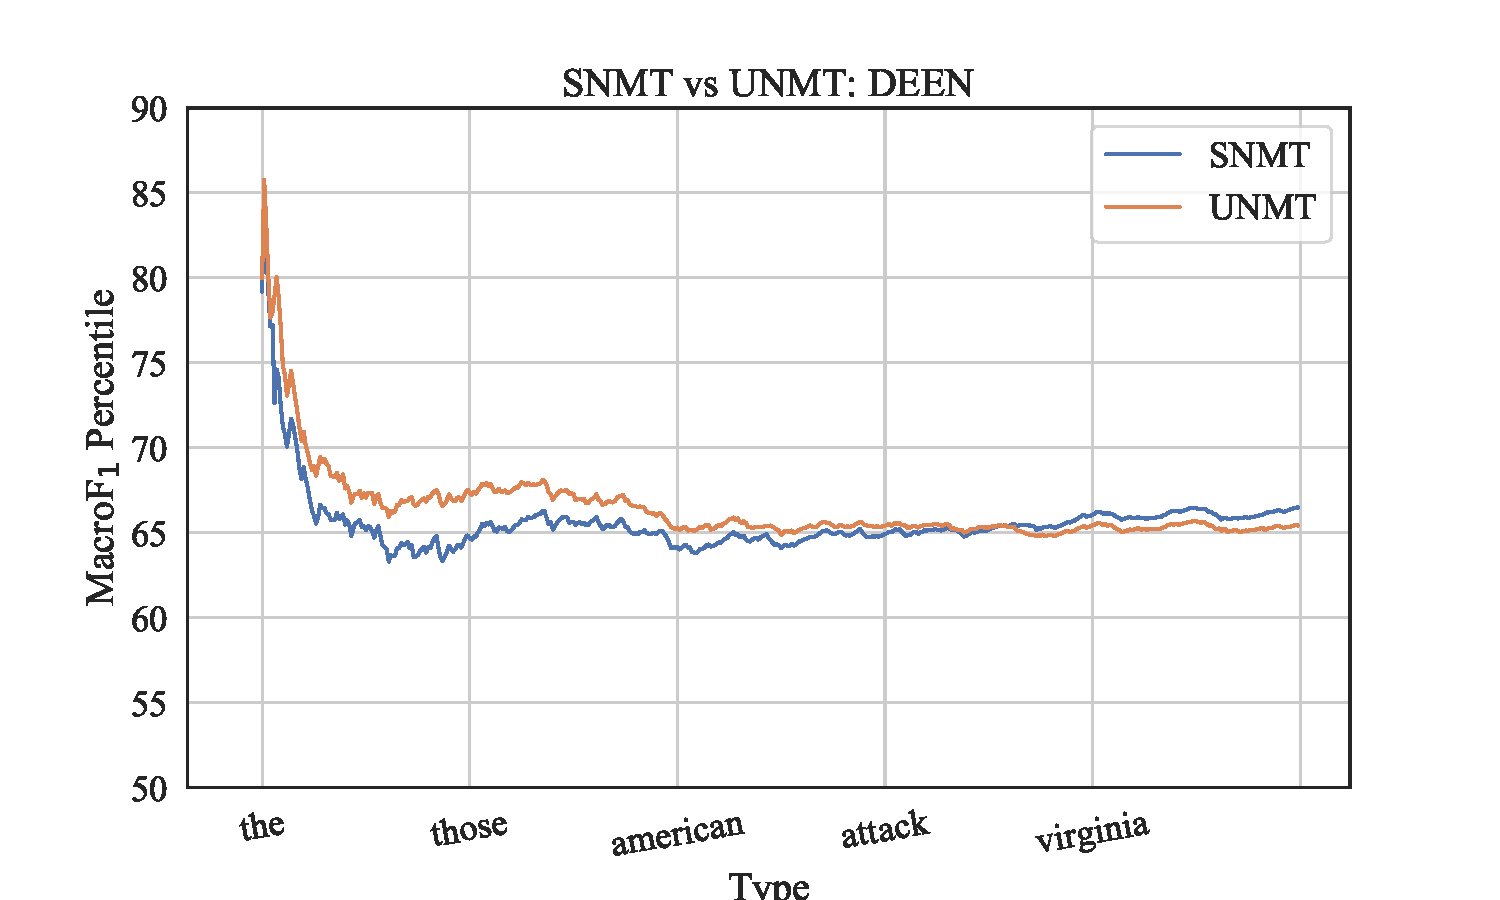
\includegraphics[width=\linewidth,trim={13mm 5mm 25mm 10mm},clip]{macroavg/s_unmt-deen-maf1.pdf}
    \end{subfigure}
    \begin{subfigure}[b]{0.495\linewidth}
    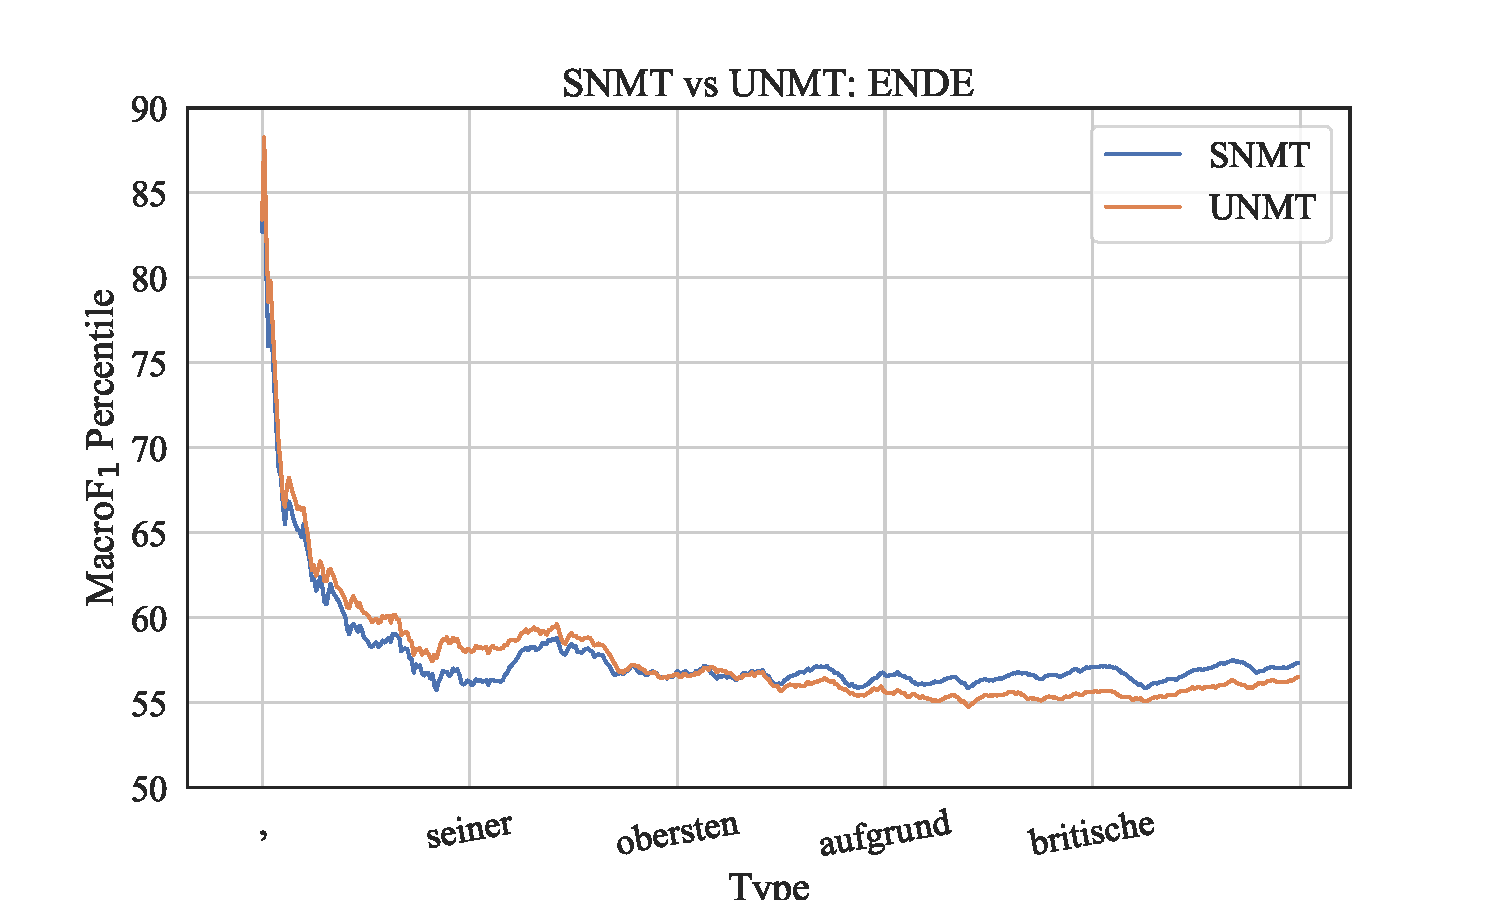
\includegraphics[width=\linewidth,trim={13mm 7mm 25mm 10mm},clip]{macroavg/s_unmt-ende-maf1.pdf}
    \end{subfigure}
    
    \begin{subfigure}[b]{0.495\linewidth}
    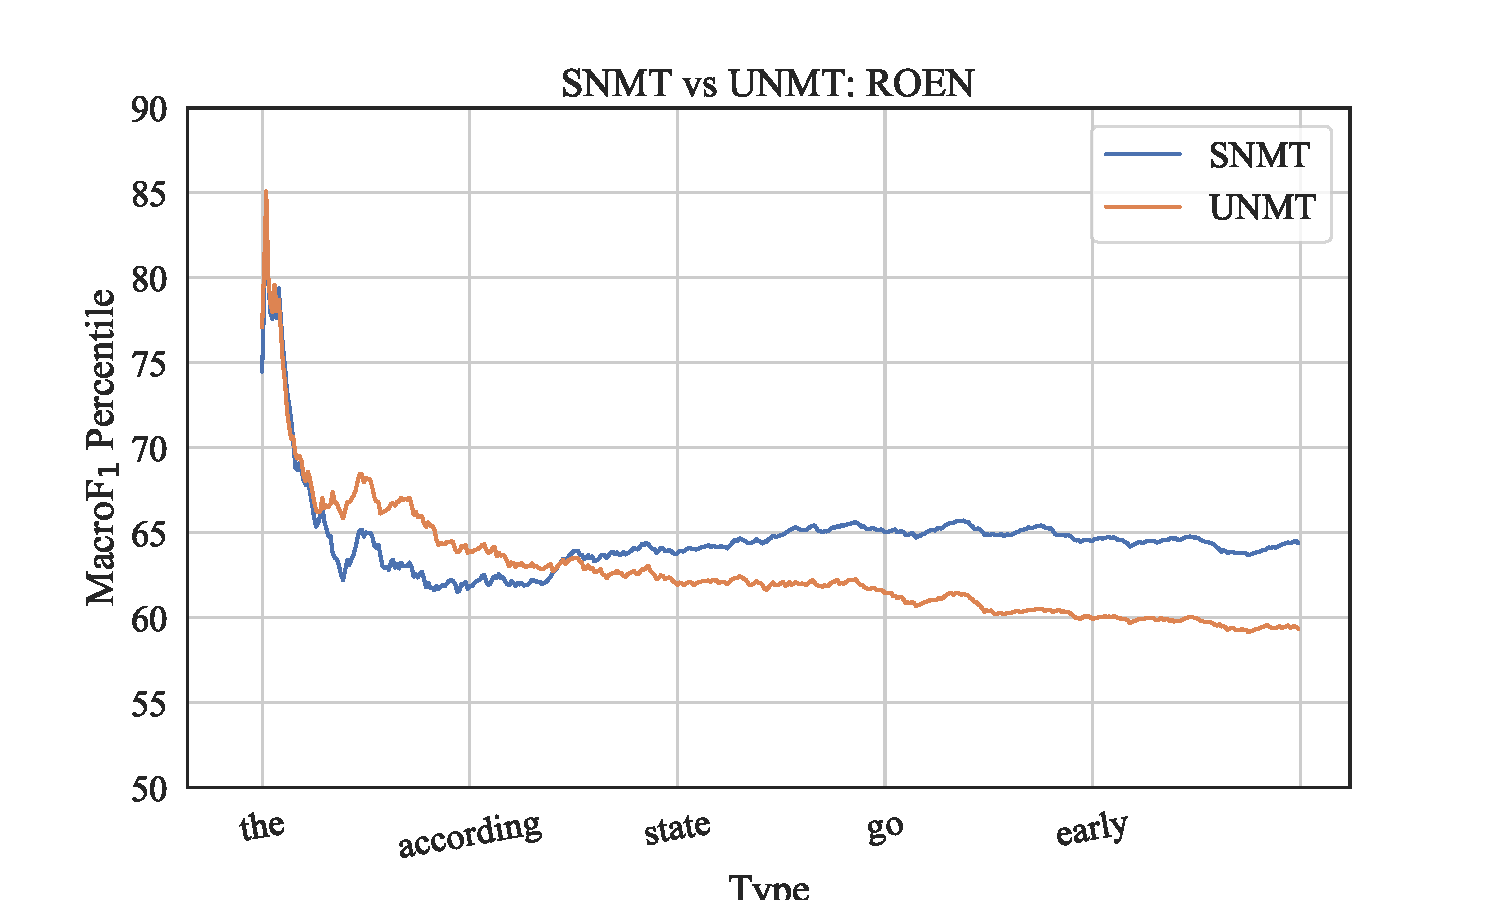
\includegraphics[width=\linewidth,trim={13mm 5mm 25mm 10mm},clip]{macroavg/s_unmt-roen-maf1.pdf}
    \end{subfigure}
    \begin{subfigure}[b]{0.495\linewidth}
      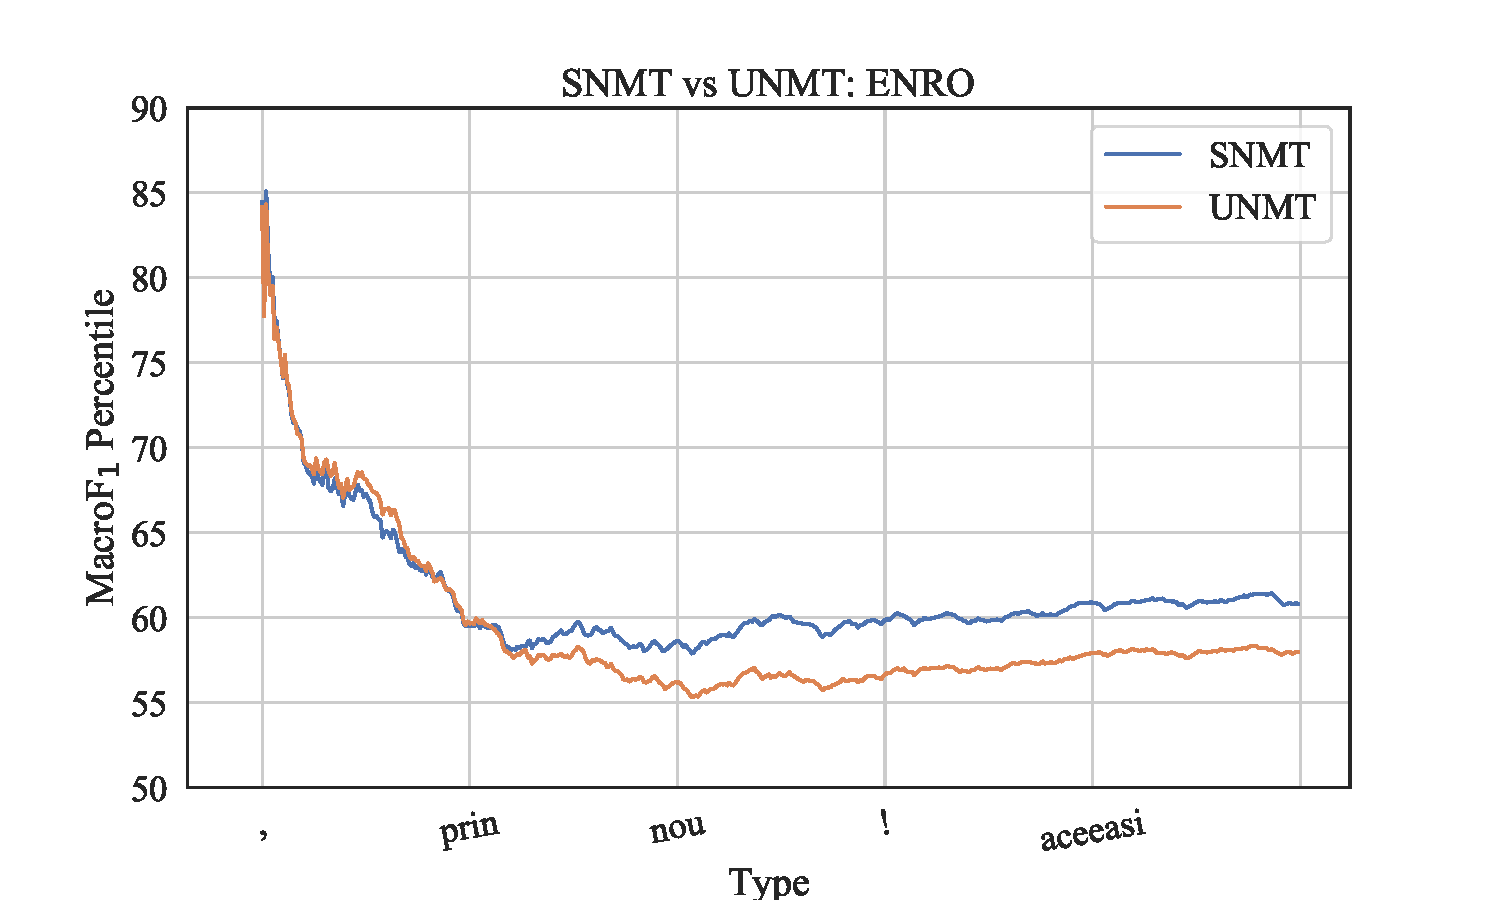
\includegraphics[width=\linewidth,trim={13mm 7mm 25mm 10mm},clip]{macroavg/s_unmt-enro-maf1.pdf}
      %\label{fig:snmt_vs_unmt_rest}
      %\caption{(Continued from Figure~\ref{fig:snmt_vs_unmt}) Visualization of \maf1 between SNMT and UNMT .  }
    \end{subfigure}
     
\caption{SNMT vs UNMT \maf1 on the most frequent 500 types.
UNMT outperforms SNMT on frequent types that are weighed heavily by \bleu\, however, SNMT is generally better than UNMT on rare types; hence, SNMT has a higher \maf1.
Only the most frequent 500 types are visualized in this figure.
}
\label{fig:snmt_vs_unmt}
\end{figure} 



%%%%%%% Appendix %%%%%%%%%%
\section{Metrics Reproducibility}
\label{sec:appmetrics}

\bleu\ scores reported in this work are computed with the \textsc{SacreBleu} library and have signature \texttt{\small BLEU+case.mixed+lang.<xx>-<yy>+numrefs.1+smooth.exp+tok.<TOK>+version.1.4.13}, where \texttt{<TOK>} is \texttt{zh} for Chinese, and \texttt{13a} for all other languages. \maf1 and \mif1 use the same tokenizer as \bleu.
\chrf1 is also obtained using \textsc{SacreBleu} and has signature \texttt{\small chrF1+lang.<xx>-<yy>+numchars.6 +space.false +version.1.4.13}.
BLUERT scores are from the \textit{base} model of \citet{sellam-etal-2020-bleurt}, which is fine-tuned on WMT Metrics ratings data from 2015-2018.
The BLEURT model is retrieved from \url{https://storage.googleapis.com/bleurt-oss/bleurt-base-128.zip}.

\maf1 and \mif1 are computed using our fork of \textsc{SacreBleu} as:\\
\texttt{sacrebleu \$REF -m macrof microf < \$HYP}. 
Our modification to SacreBLEU is available at \url{https://github.com/isi-nlp/sacrebleu/tree/macroavg-naacl21}; alternatively, it can be installed as \code{pip install sacrebleu-macrof}\footnote{\url{https://pypi.org/project/sacrebleu-macrof/2.0.1/}}

\section{Conclusion}
We have evaluated NLG in general and MT specifically as a multi-class classifier, and illustrated the differences between micro- and macro- averages using \mif1 and \maf1 as examples (Section~\ref{sec:mt-as-cls}).
\maf1 captures semantic adequacy better than \mif1 (Section~\ref{sec:webnlg}).
\bleu, being a micro-averaged measure, served well in an era when generating fluent text was at least as difficult as generating adequate text. Since we are now in an era in which fluency is taken for granted and semantic adequacy is a key discriminating factor, macro-averaged measures such as \maf1 are better at judging the generation quality of MT models (Section~\ref{sec:wmt-metrics}).
We have found that another popular metric, \chrf1, also performs well on direct assessment,
however, being an implicitly micro-averaged measure, it does not perform as well as \maf1 on downstream CLIR tasks (Section~\ref{sec:material}).
Unlike BLEURT, which is also adequacy-oriented, \maf1 is directly interpretable, does not require retuning on expensive human evaluations when changing language or domain, and does not appear to have uncontrollable biases resulting from data effects.
It is both easy to understand and to calculate, and is  
inspectable, enabling fine-grained analysis at the level of individual word types. These attributes make it a useful metric for understanding and addressing the flaws of current models. For instance, we have used \maf1 to compare supervised and unsupervised NMT models at the same operating point measured in \bleu, and determined that supervised models have better adequacy than the current unsupervised models (Section~\ref{sec:unmt}).

Macro-average is a useful technique for addressing the importance of the long tail of language, and \maf1 is our first step in that direction; we anticipate the development of more advanced macro-averaged metrics that take advantage of higher-order and character n-grams in the future. 


%\section*{Acknowledgements}
%The authors thank Shantanu Agarwal, Joel Barry, and Scott Miller for their help with CLSSTS CLIR experiments, and Daniel Cohen for discussions on IR evaluation methods. This research is based upon work supported by the Office of the Director of National Intelligence (ODNI), Intelligence Advanced Research Projects Activity (IARPA), via AFRL Contract FA8650-17-C-9116.  The views and conclusions contained herein are those of the authors and should not be interpreted as necessarily representing the official policies or endorsements, either expressed or implied, of the ODNI, IARPA, or the U.S. Government. The U.S. Government is authorized to reproduce and distribute reprints for Governmental purposes notwithstanding any copyright annotation thereon.


\section*{Ethical Consideration}
Since many ML models including NMT are themselves opaque and known to possess data-induced biases~\cite{prates2019-mt-bias}, using opaque and biased evaluation metrics in concurrence makes it even harder to discover and address the flaws in modeling.
Hence, we have raised concerns about the opaque nature of the current model-based evaluation metrics, and demonstrated examples displaying unwelcome biases in evaluation. We advocate the use of the \maf1 metric, as it is easily interpretable and offers the explanation of score as a composition of individual type performances.
In addition, \maf1 treats all types equally, and has no parameters that are directly or indirectly estimated from data sets. Unlike \maf1, \mif1 and other implicitly or explicitly micro-averaged metrics assign lower importance to rare concepts and their associated rare types. 
The use of micro-averaged metrics in real world evaluation could lead to marginalization of rare types.

\textit{Failure Modes:}
The proposed \maf1 metric is not the best measure of fluency of text. 
Hence, we suggest caution while using \maf1 to draw fluency related decisions. \maf1 is inherently concerned with \textit{words}, and assumes the output language is easily segmentable into word tokens. Using \maf1 to evaluate translation into alphabetical languages such as Thai, Lao, and Khmer, that do not use white space to segment words, requires an effective tokenizer. Absent this the method may be ineffective; we have not tested it on languages beyond those listed in Section~\ref{sec:wmt-metrics}.

\textit{Reproducibility:}
Our implementation of \maf1 and \mif1 has the same user experience as \bleu{} as implemented in \textsc{SacreBleu}; signatures are provided in Section~\ref{sec:appmetrics}. 
In addition, our implementation is  computationally efficient, and has the same (minimal) software and hardware requirements as \bleu{}. 
 All data for MT and NLG human correlation studies is publicly available and documented. Data for reproducing the IR experiments in Section~\ref{sec:lignos-etal} is also publicly available and documented. The data for reproducing the IR experiments in Section~\ref{sec:material} is only available to participants in the CLSSTS shared task. 

\textit{Climate Impact:} Our proposed metrics are on par with \bleu{} and such model-free methods, which consume significantly less energy than most model-based evaluation metrics.



\chapter{Imbalanced Classification Learning}
\label{ch:imb-learning}


\section{Data based Methods}
\subsection{Sampling Methods}
These are similar to quota systems. 
\begin{enumerate}
    \item Random Up-sample or Over-sample Minority
    \item Random Down-sample or Under-sample Majority
\end{enumerate}


\subsection{Augmentation Methods}

\begin{enumerate}
 \item Synthetic Minority Over-sample Technique (SMOTE): \citet{chawla2002smote}
 \item Just add more data: law of diminishing returns favor minority classes more than majority classes. \citet{koehn2017sixchallenges} learning curve.
\end{enumerate}


%%%%%%%%%%%%%%%%%%%%
\section{Unequal Objectives}
Preference based methods.

Cross Entropy (CE) is the de-facto objective for deep learning classification models.
Consider a dataset of $N$ examples, $$ D = \{(x^{(i)}, y^{(i)}) | i = 1, 2, 3, ... N\}$$
where, ($x^{(i)}, y^{(i)})$ be (input, label), respectively.

Let $p^(i)_c=p(y^{(i)}_c|x^{(i)})$ be model's output probability.

CE between $y^{(i)}$ and $p^{(i)}$ (i.e., on an example $i$) is:

\begin{equation}
 CE^{(i)} = -\sum^C_{c} y^{(i)}_c\cdot \log(p^{(i)}_c)
\end{equation}
Often, $y^{(i)}$ is a one-hot vector of $C$ classes: $\{y_1, y_2, ... y_C\}$, which zero-out all but one terms in the above summation. However, we retain the generalization due to $y^{(i)}$ sometimes being non one-hot distribution, such as the label smoothing case (Section \ref{sec:label-smooth}).

Models are generally optimized using batch gradient descent, hence, the mean CE on a batch of examples:

\begin{equation} \label{eqn:ce-batch}
 CE = - \frac{1}{N} \sum^N_{i=1}\sum^C_{c=1} y^{(i)}_c\cdot \log(p^{(i)}_c)
\end{equation}

\subsection{Weighted Cross Entropy (wCE)} is a simple way of addressing imbalanced classes by assigning unequal weights to classes.

\begin{equation} \label{eqn:wce-batch}
 wCE = -\frac{1}{N} \sum^N_{i=1} \sum^C_{c=1} w_c \cdot y^{(i)}_c \cdot \log(p^{(i)}_c)
\end{equation}
where $w_c$ is the weight associated with class $c$.
Equation (\ref{eqn:ce-batch}) is a special case of (\ref{eqn:wce-batch}), obtained by  equal weights to all classes, i.e., $\forall c, w_c=1$.

Weights can either be manually set or obtained using heuristics based on training data statistics, which are described in the following sections.
Let $f_c$ be class $c$'s frequency in the training data; $\sum_{c=1}^C f_c = N$. 
The following statistics are used for obtaining weights from frequency:

\begin{enumerate}
\item \textit{\textbf{Inverse Frequency:}}
\begin{equation}
 w_c \propto 1/f_c;\hspace{6mm} w_c = k/f_c
\end{equation}
Where $k$ is proportionality constant, usually min, median or max of $f$.

\item \textit{\textbf{Inverse Log Frequency:}}
\begin{equation}
 w_c \propto 1/\log(f_c); \hspace{6mm} w_c = k/\log(f_c)
\end{equation}

\item \textit{\textbf{Inverse Square Root Frequency}}:
\begin{equation}
 w_c \propto 1/\sqrt{f_c};\hspace{6mm} w_c = k/\sqrt{f_c}
\end{equation}


\item \textit{\textbf{Effective Number of Samples}:}\\
\citet{cui2019effective-samples} argue that the use of raw frequencies for weighing (such as with inverse frequency) is detrimental to model performance. 
They propose effective number of samples for class $c$,  $1 \le E_c \le f_c $ , as an exponential function of $\beta \in [0,1)$, as

$$E_c = \frac{1-\beta^{f_c}}{1-\beta}$$ 
where $f_c$ is the raw frequency of class $c$ in training data.
If $\beta=0$, $E_c=1$ and as $\beta\rightarrow1$, $E_c \rightarrow f_c$.

\begin{equation}
    w_c \propto \frac{1}{E_c}; \hspace{4mm} w_c = k\cdot \frac{1-\beta}{1-\beta^{f_c}}
\end{equation}
for some constant, $k > 0$.

They also offer geometrical interpretation for $\beta=(N-1)/N$, where $N \ge 1$ is the volume of a hyper-space that can contain all the examples. 

\end{enumerate}


%https://www.desmos.com/calculator/xjedqqsbpm
%begin{figure}
%    \centering
%    \includegraphics[width=\linewidth]{weight-fn.png}
%    \caption{Weight functions}
%    \label{fig:weight-fn-viz}
%\end{figure}


\subsection{Focal Loss}
\label{sec:focal-loss}
 Focal loss \cite{lin-etal-2020-focalloss} assigns higher loss for harder-to-learn examples.
 Implicit assumption is that minority classes are harder to learn than the majority classes.
Given $\gamma \ge 0$,
\begin{equation}
    FL^{(i)} = -\sum^C_{c=1} y^{(i)}_c \cdot (1-p^{(i)}_c)^\gamma \cdot \log(p^{(i)}_c) 
\end{equation}
However, noisy examples may have adverse effect on loss landscape (refer to \citet{cui2019effective-samples}).

\section{Label Smoothing}
\label{sec:label-smooth}
Label smoothing \cite{szegedy2016re-inception} is a regularization technique.
Given a hyper parameter $0 \le \varepsilon \le 1$, the ground truth $y$ is transformed from one-hot vector to a smooth distribution, as:
\begin{equation}
    y_c^* = \begin{cases}
     1-\varepsilon & \text{if } y_c = 1 \\
     \frac{\varepsilon}{C-1} & \text{otherwise, i.e. if } y_c=0
    \end{cases}
\label{eqn:label_smooth}
\end{equation}
Intuitively, $\varepsilon$ quantity of probability mass is moved from the correct class (i.e $y_c=1$) and evenly distributed to all other classes (i.e. $y_c=0)$.
All the benefits of label smoothing are not well understood; e.g. \citet{muller-2019-when-labelsmooth} show that label smoothing helps in tighter label cluster formation in hidden space, and model calibration.
We conjecture that label smoothing may also be helping imbalanced classes. 
With the smoothing transformation, though all classes gain equal quantity of probability mass, the classes that occur more frequently lose more mass compared to classes that occur only rarely. 

When combined with weighted cross entropy:
\begin{equation}
 lswCE^{(i)} = -\sum^C_{c=1} w_c \cdot y^{*(i)}_c \cdot \log(p^{(i)}_c)
\end{equation}


\section{Proposed Methods}

In this section, we describe our proposed methods for imbalanced learning.
\subsection{Information Content as Weights}

\cite{shannon1948mathematical}
\begin{equation}
   w_c = -\log_2(\pi_c)
\end{equation}
where $\pi_c$ is probability of class $c$ in training (i.e. prior), obtained as: $$\pi_c = \frac{f_c}{\sum^C_{c'=1}f_{c'}}$$\\


\subsection{Macro Cross Entropy}
Modify the loss function; take macro average

Currently, the weighted CE is:
\begin{equation*}
 wCE = -\frac{1}{N} \sum^N_{i=1} \sum^C_{c=1} w_c \cdot y^{(i)}_c \cdot \log(p^{(i)}_c)
\end{equation*}


We define \textbf{Macro CE} as
\begin{equation} \label{eqn:mCE-batch}
  mCE = -\sum^C_{c=1} \frac{1}{\sum^{N}_{j=1} y^{(j)}_c} \sum^N_{i=1} y^{(i)}_c \cdot \log(p^{(i)}_c)
\end{equation}

If the labels are one-hot vectors, then $\sum^{N}_{j=1} y^{(j)}_c = f_c$. 
Note that, Macro CE (\ref{eqn:mCE-batch}) is equivalent, in theory, to Weighted CE (\ref{eqn:wce-batch}) with $w_c = 1/\sum^{N}_{j=1} y^{(j)}_c$.
Macro CE easily adapts to the imbalance in each min-batch as well as to the smoothed labels, where as Weighted CE has global weights and do not account for smoothed labels.

\subsection{Balanced Label Smoothing}
Let $w_c$ be the weight of class such that $\forall c, w_c > 0$ and $\sum_c w_c = 1$.

Instead of distributing $\varepsilon$ evenly across all other classes, distribute more quantity to the heavily weighted classes (such as the rare ones), and less to the lightly weighted classes. 
 Let $c$ be a class with $y_c=1$ from which $\varepsilon$ quantity of probability mass is moved out.
 
 Let $d$ be another class that receives, i.e., $d \ne c$ and $y_d=0$.  
  Instead of $y^*_d = \frac{1}{C-1} \cdot \varepsilon$, as in Equation (\ref{eqn:label_smooth}), $y^*_d = w_d \cdot \varepsilon$. 
  
  For simplicity\footnote{to ensure $\sum_i y^*_i = 1$}, $y^*_c = 1-\varepsilon + w_c \cdot \varepsilon = 1-\varepsilon(1-w_c)$
  

Related: Adaptive label smoothing \cite{wang-2021-adalabel}

\chapter{Applications}
\label{ch:applications}

\section{Multilingual Translation: 500 Languages to English}

Neural machine translation (NMT)~\cite{bahdanau2014nmtattn,vaswani2017attention} has progressed to reach human performance on select benchmark tasks~\cite{barrault-etal-2019-findings,barrault-etal-2020-findings}. 
However, as MT research has mainly focused on translation between a small number of high resource languages, the unavailability of usable-quality translation models for low resource languages remains an ongoing concern.
Even those commercial translation services attempting to broaden their language coverage has only reached around one hundred languages; this excludes most of the thousands of languages used around the world today.

Freely available corpora of parallel data for many languages are available, though they are hosted at various sites, and are in various forms. A challenge for incorporating more languages into MT models is a lack of easy access to all of these datasets.While standards like ISO 639-3 have been established to bring consistency to the labeling of language resources, these are not yet widely adopted.
In addition, scaling experimentation to several hundred languages on large corpora involves a significant engineering effort.
Simple tasks such as dataset preparation, vocabulary creation, transformation of sentences into sequences, and training data selection becomes formidable at scale due to corpus size and heterogeneity of data sources and file formats.
We have developed tools to precisely address all these challenges, which we demonstrate in this work.
 
Specifically, we offer three tools which can be used either independently or in combination to advance NMT research on a wider set of languages (Section \ref{sec:tools}): firstly, \mtdata, which helps to easily obtain parallel datasets (Section \ref{sec:mtdata}); secondly, \nlcodec, a vocabulary manager and storage layer for transforming sentences to integer sequences, that is efficient and scalable (Section \ref{sec:nlcodec}); and lastly, \rtg, a feature-rich Pytorch-backed NMT toolkit that supports reproducible experiments (Section \ref{sec:rtg}).

We demonstrate the capabilities of our tools by preparing a massive bitext dataset with more than 9 billion tokens per side, and training a single multilingual NMT model capable of translating 500 source languages to English (Section \ref{sec:500-eng}).
We show that the multilingual model is usable either as a service for translating several hundred languages to English (Section \ref{sec:value.off-shelf-mt}), or as a parent model in a transfer learning setting for improving translation of low resource languages (Section \ref{sec:value.transfer-learning}). 
%pretrained multilingual embeddings (Section \ref{sec:value.embeddings}),


\section{Tools}
\label{sec:tools}
 Our tools are organized into the following sections:

\begin{comment}
Specifically, \textsc{MTData} (Section \ref{sec:mtdata}) is useful for preparing training data for hundreds of languages, 
\textsc{NLCodec} (section \ref{sec:nlcodec}) is useful for efficiently proprocessing, storing, and accessing the training data,
and \textsc{RTG} (section \ref{sec:rtg}) NMT toolkit for training an MT model. 
In addition, all these tools are built with reproducibility and usability in mind. 
These tools have been made publicly available, with permissive open source licenses.
We hope these tools help advance MT efforts beyond the top few high resource languages. 
\end{comment}

\subsection{\textsc{MTData}}
\label{sec:mtdata}
\textsc{MTData} addresses an important yet often overlooked challenge -- dataset preparation. 
By assigning an ID for datasets, we establish a clear way of communicating the exact datasets used for MT experiments, which helps in reproducing the experimental setup.
By offering a unified interface to datasets from many heterogeneous sources, \mtdata\ hides mundane tasks such as locating URLs, downloading, decompression, parsing, and sanity checking. Some noteworthy features are:
\begin{itemize}[noitemsep,topsep=0pt,leftmargin=4mm]
\item \textit{Indexer}: a large index of publicly available parallel datasets.
\item \textit{Normalizer:} maps language names to ISO-639-3 codes which has representation space for 7800+ languages.\footnote{\url{https://iso639-3.sil.org}}
\item \textit{Parsers:} parses heterogeneous data formats for parallel datasets, and produces a simple plain text file by merging all the selected datasets.
\item \textit{Extensible:} new datasets and parsers can be easily added.
\item \textit{Local Cache}: reduces network transfers by maintaining a local cache, which is shared between experiments.
\item \textit{Sanity Checker}: performs basic sanity checks such as segment count matching and empty segment removal. When error states are detected, stops the setup with useful error messages.
\item \textit{Reproducible:} stores a signature file that can be used to recreate the dataset at a later time.
\item \textit{Courtesy:} shows the original \BibTeX\ citation attributed to datasets.
\item \textit{Easy Setup:} \texttt{pip install mtdata}
\item \textit{Open-source:} \\ \url{https://github.com/thammegowda/mtdata}
\end{itemize}

Listing \ref{lst:mtdata-eg} shows an example for listing and getting datasets for German-English.
\begin{listing}
\begin{minted}[baselinestretch=1, fontsize=\footnotesize, frame=lines, framesep=2mm,]{bash}
# List all the available datasets for deu-eng
$ mtdata list -l deu-eng
# Get the selected training & held-out sets
$ mtdata get -l deu-eng --merge\
 -tr wmt13_europarl_v7 wmt13_commoncrawl\ 
    wmt18_news_commentary_v13\
 -ts newstest201{8,9}_deen -o data
\end{minted}
\caption{\mtdata\ examples for listing and downloading German-English datasets.
The \texttt{--merge} flag results in merging all of the training datasets specified by \texttt{-tr} argument into a single file. }
\label{lst:mtdata-eg}
\end{listing}
 In Section~\ref{sec:datasets}, we use \mtdata\footnote{At the time of writing, v0.2.8} to obtain thousands of publicly available datasets for a large many-to-English translation experiment.

\subsection{\nlcodec}
\label{sec:nlcodec}
\nlcodec\ is a vocabulary manager with encoding-decoding schemes to transform natural language sentences to and from integer sequences.\\
\textbf{Features:}
\begin{itemize}[noitemsep,topsep=0pt,leftmargin=4mm]
\item \textit{Versatile:} Supports commonly used vocabulary schemes such as characters, words, and byte-pair-encoding (BPE) subwords~\cite{sennrich-etal-2016-bpe}.
\item \textit{Scalable:} Apache Spark\footnote{\url{https://spark.apache.org/}}\cite{zaharia2016spark} backend can be optionally used to create vocabulary from massive datasets.
\item \textit{Easy Setup:} \texttt{pip install nlcodec} 
\item \textit{Open-source:}\\ \url{https://github.com/isi-nlp/nlcodec/}
\end{itemize}

When the training datasets are too big to be kept in the primary random access memory (RAM), the use of secondary storage is inevitable.
The training processes requiring random examples lead to random access from a secondary storage device.
Even though the latest advancements in secondary storage technology such as solid-state drive (SSD) have faster serial reads and writes, their random access speeds are significantly lower than that of RAM. 
%In addition, since sentences are of variable lengths, use of fixed sized tensors are not feasible. 
To address these problems, we include an efficient storage and retrieval layer, \nldb, which has the following features:
\begin{itemize}[noitemsep,topsep=0pt,leftmargin=4mm]
  \item \textit{Memory efficient} by adapting datatypes based on vocabulary size. For instance, encoding with vocabulary size less than 256 (such as characters) can be efficiently represented using 1-byte unsigned integers. Vocabularies with fewer than 65,536 types, such as might be generated when using subword models \cite{sennrich-etal-2016-bpe} require only 2-byte unsigned integers, and 4-byte unsigned integers are sufficient for vocabularies up to 4 billion types. 
As the default implementation of Python, CPython, uses 28 bytes for all integers, we accomplish this using NumPy~\cite{harris2020numpy}. This optimization makes it possible to hold a large chunk of training data in smaller RAM, enabling a fast random access.
  \item \textit{Parallelizable:} Offers a multi-part database by horizontal sharding that supports parallel writes (e.g., Apache Spark) and parallel reads (e.g., distributed training).
%  \item \textit{I/O efficient:} Reads and writes large blocks at once instead of multiple smaller chunks, thus taking advantage of faster serial reads and write speeds.
  \item Supports commonly used batching mechanisms such as random batches with approximately-equal-length sequences.
\end{itemize}

\nldb\ has a minimal footprint and is part of the \nlcodec\ package.
In Section~\ref{sec:500-eng}, we take advantage of the scalability and efficiency aspects of \nlcodec\ and \nldb\ to process a large parallel dataset with 9 billion tokens on each side.


\subsection{\rtg}
\label{sec:rtg}
Reader translator generator (\rtg) is a neural machine translation (NMT) toolkit based on Pytorch~\cite{NEURIPS2019_Pytorch}. 
Notable features of \rtg\ are:
\begin{itemize}[noitemsep,topsep=0pt,leftmargin=4mm]
\item \textit{Reproducible:} All the required parameters of an experiment are included in a single YAML configuration file, which can be easily stored in a version control system such as \texttt{git} or shared with collaborators.
\item Implements Transformer~\cite{vaswani2017attention}, and recurrent neural networks (RNN) with cross-attention models ~\cite{bahdanau2014nmtattn,luong2015effectiveAttn}.
%cho2014GRU,hochreiter1997LSTM
\item Supports distributed training on multi-node multi-GPUs, gradient accumulation, and Float16 operations.
\item Integrated Tensorboard helps in visualizing training and validation losses. 
% shows training speed, estimated finish time on \texttt{tqdm} progress-bar. 
\item Supports weight sharing~\cite{press-wolf-2017-embeddings}, parent-child transfer~\cite{zoph-etal-2016-transfer}, beam decoding with length normalization~\cite{wu-etal-2016-GNMT}, early stopping, and checkpoint averaging. 
%, and transfer learning with selective layer weight freezing. 
\item Flexible vocabulary options with \nlcodec\ and \sentpiece~\cite{kudo-richardson-2018-sentencepiece} which can be either shared or separated between source and target languages.
\item \textit{Easy setup:} \texttt{pip install rtg}
%\item A CLI for running end-to-end experiments based on a YAML config file (\texttt{rtg-pipe}); also supports experiment forking and export (\texttt{rtg-fork}, \texttt{rtg-export}).
%\item In addition to CLI interface for translation generation (\texttt{rtg-decode}), web and REST interfaces are also supported (\texttt{rtg-serve}).
\item \textit{Open-source:} \url{https://isi-nlp.github.io/rtg/}
\end{itemize}

\begin{comment}
% [
%frame=lines,
%framesep=2mm,
% baselinestretch=1.1,
% fontsize=\footnotesize,
%linenos
%]{bash}
\begin{listing}[ht]
\scriptsize
%\tiny
\inputminted{yaml}{sample-conf.yml}
\caption{An example \textit{conf.yml} file from an RTG experiment.}
\end{listing}


\begin{table}[]
    \centering
    \footnotesize
    \begin{tabular}{l  l| r r}
        NMT & BPE Impl  & NewsTest18 & NewsTest19 \\ \hline \hline
        \rtg & \nlcodec\   & 32.6   & 29.0 \\
        \rtg & \scriptsize{\sentpiece\ }& 32.3 & 28.7 \\
        FairSeq & subword-nmt & & \\
        T2T &  (built-in) & &
    \end{tabular}
    \caption{Transformer-base model is trained on the datasets shown in Listing~\ref{lst:mtdata-eg} for 200K optimizer updates having a batch size of 4200 tokens. All models use shared 8000 BPE subwords as vocabulary. The BLEU scores are from \sacrebleu\ \texttt{BLEU+c.mixed+l.de-en+\#.1+s.exp+
    t.wmt1\{8,9\}+tok.13a+v.1.4.13}.  }
    \label{tab:my_label}
\end{table}

\end{comment}



\section{Many-to-English Multilingual NMT}
\label{sec:500-eng}
In this section, we demonstrate the use of our tools by creating a massively multilingual NMT model from publicly available datasets. 

\subsection{Dataset}
\label{sec:datasets}
We use \mtdata\ to download datasets from various sources, given in Table~\ref{tab:data-sources}. 
To minimize data imbalance, we select only a subset of the datasets available for high resource languages, and select all available datasets for low resource languages. The selection is aimed to increase the diversity of data domains and quality of alignments. 

 \begin{table}[ht]
 \centering
 %\footnotesize
 \begin{tabular}{p{0.3\linewidth} p{0.7\linewidth}}
  Dataset   & Reference \\ \hline\hline
 Europarl    & \citet{koehn2005europarl} \\
 KFTT Ja-En & \citet{neubig11kftt}  \\ 
 Indian6     & \citet{post-etal-2012-constructing}   \\ 
 OPUS        & \citet{tiedemann-2012-parallel}  \\
 UNPCv1     & \citet{ziemski-etal-2016-unpc}   \\
 Tilde MODEL & \citet{rozis-skadins-2017-tilde}  \\
 TEDTalks    & \citet{qi-etal-2018-pretrainemb}  \\ 
 IITB Hi-En & \citet{kunchukuttan-etal-2018-iit} \\
 Paracrawl   & \citet{espla-etal-2019-paracrawl} \\
 WikiMatrix & \citet{schwenk-etal-2019-wikimatrixv1} \\
 JW300       & \citet{agic-vulic-2019-jw300}  \\
 PMIndia & \citet{haddow2020pmindia}  \\
 OPUS100    & \citet{zhang-etal-2020-multiling-nmt} \\
 WMT [13-20] & \citet{bojar-etal-2013-findings, bojar-etal-2014-findings, bojar-etal-2015-findings, bojar-etal-2016-findings, bojar-etal-2017-findings, bojar-etal-2018-findings, barrault-etal-2019-findings, barrault-etal-2020-findings} \\

 \end{tabular}
 \caption{Various sources of MT datasets.}
 \label{tab:data-sources}
\end{table}

%\begin{figure*}[ht]
\begin{sidewaysfigure}
\centering
    %trim={5mm 4mm 5mm 5mm},clip
    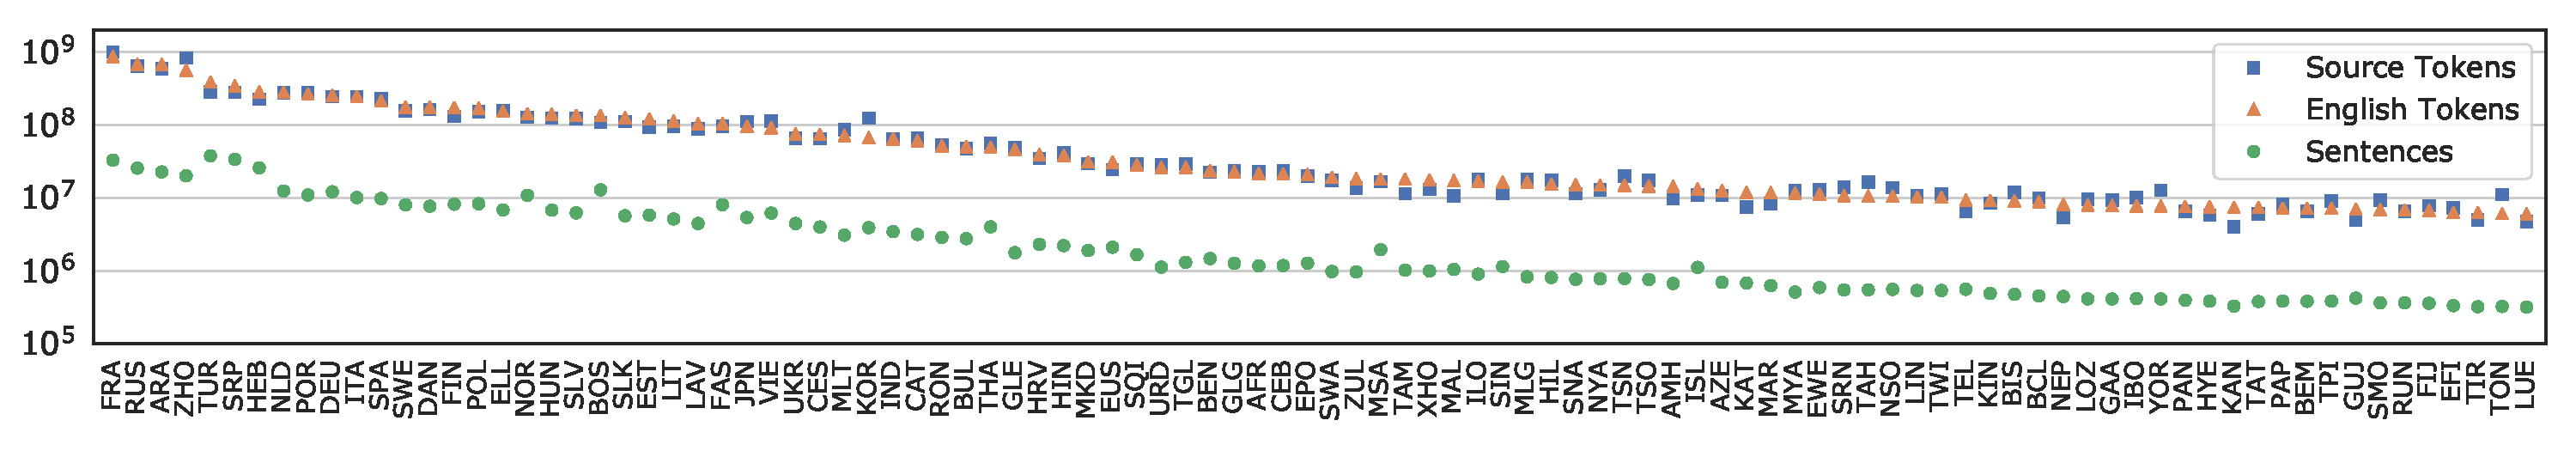
\includegraphics[height=0.14\vsize,trim={5mm 4mm 5mm 5mm},clip]{manyeng/lang-stats-1-100.pdf}
    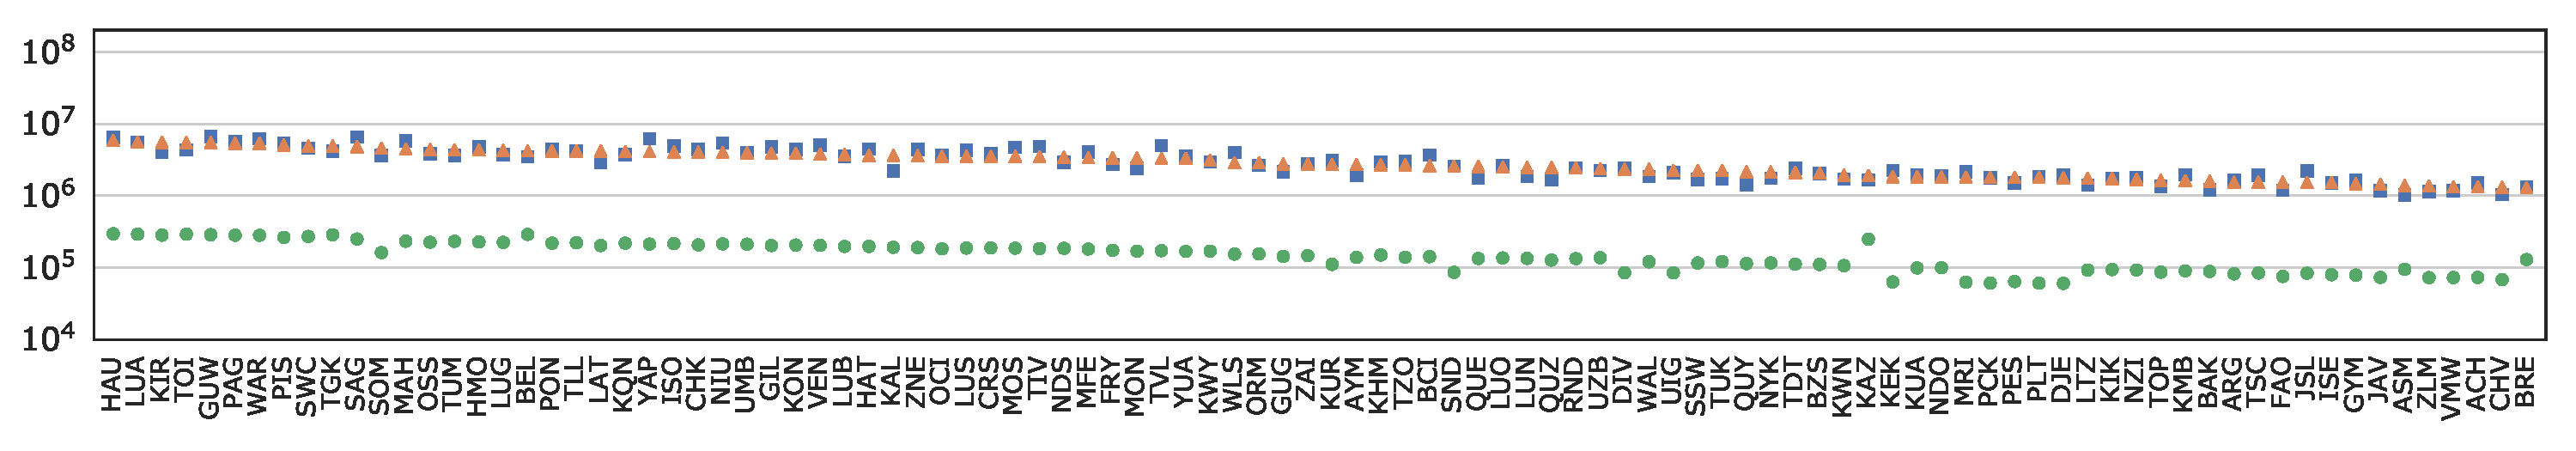
\includegraphics[height=0.14\vsize,trim={5mm 4mm 5mm 5mm},clip]{manyeng/lang-stats-101-200.pdf}
    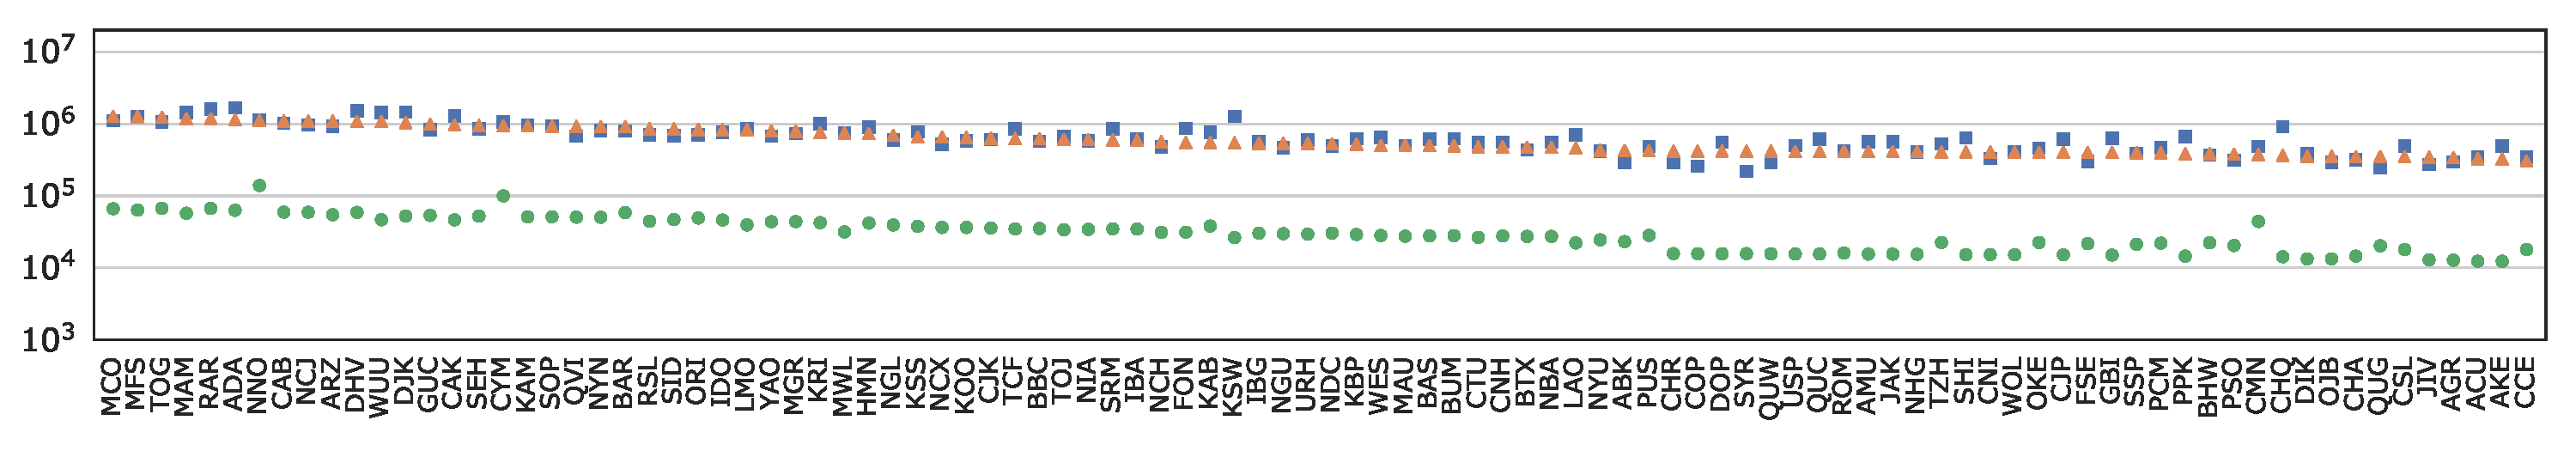
\includegraphics[height=0.14\vsize,trim={5mm 4mm 5mm 5mm},clip]{manyeng/lang-stats-201-300.pdf}
    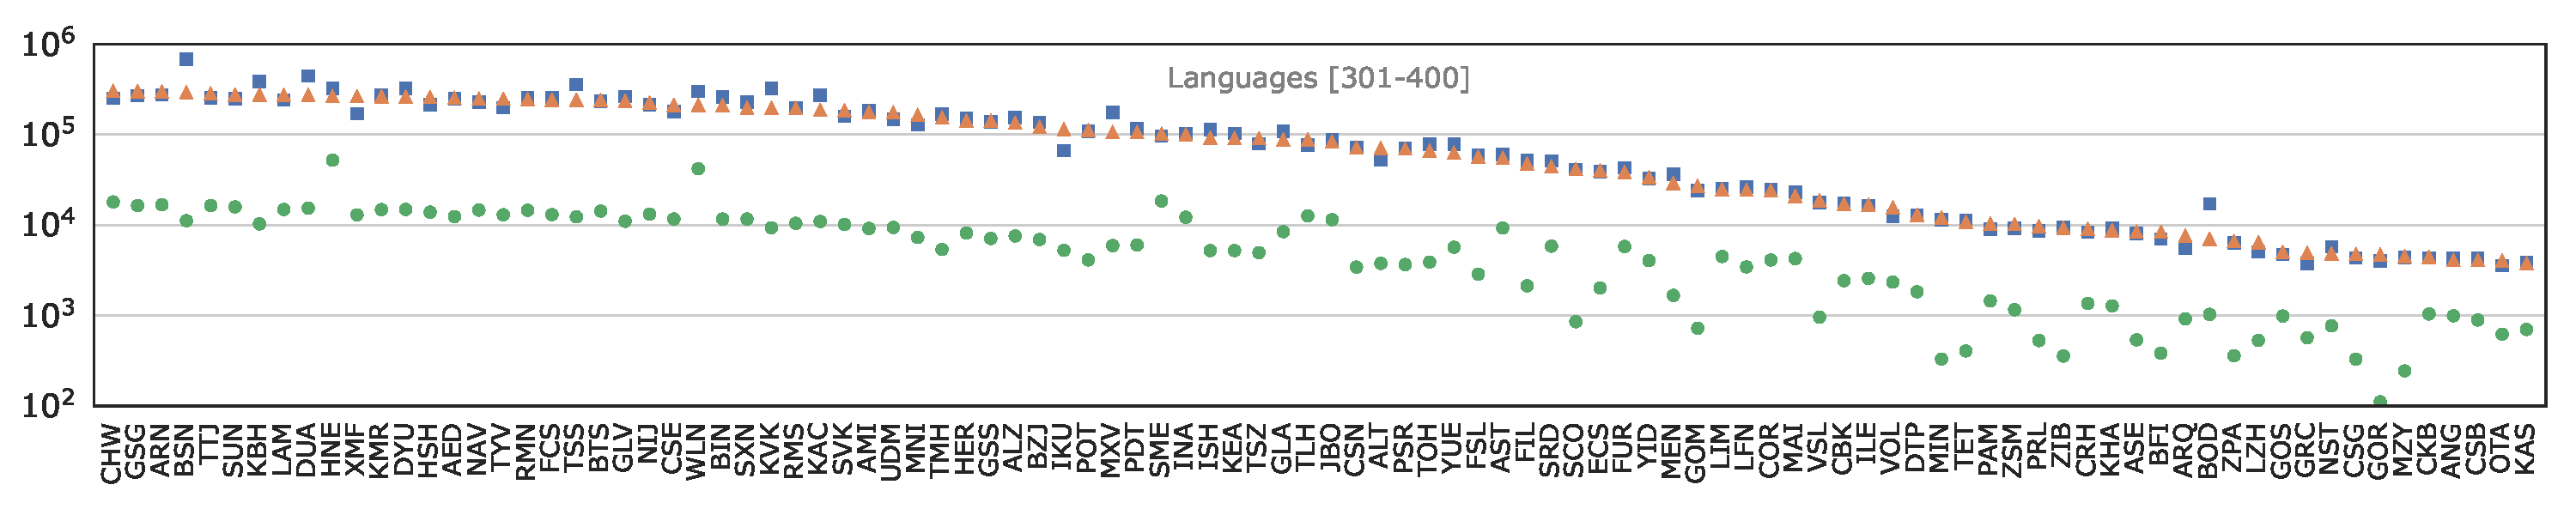
\includegraphics[height=0.14\vsize,trim={5mm 4mm 5mm 5mm},clip]{manyeng/lang-stats-301-400.pdf}
    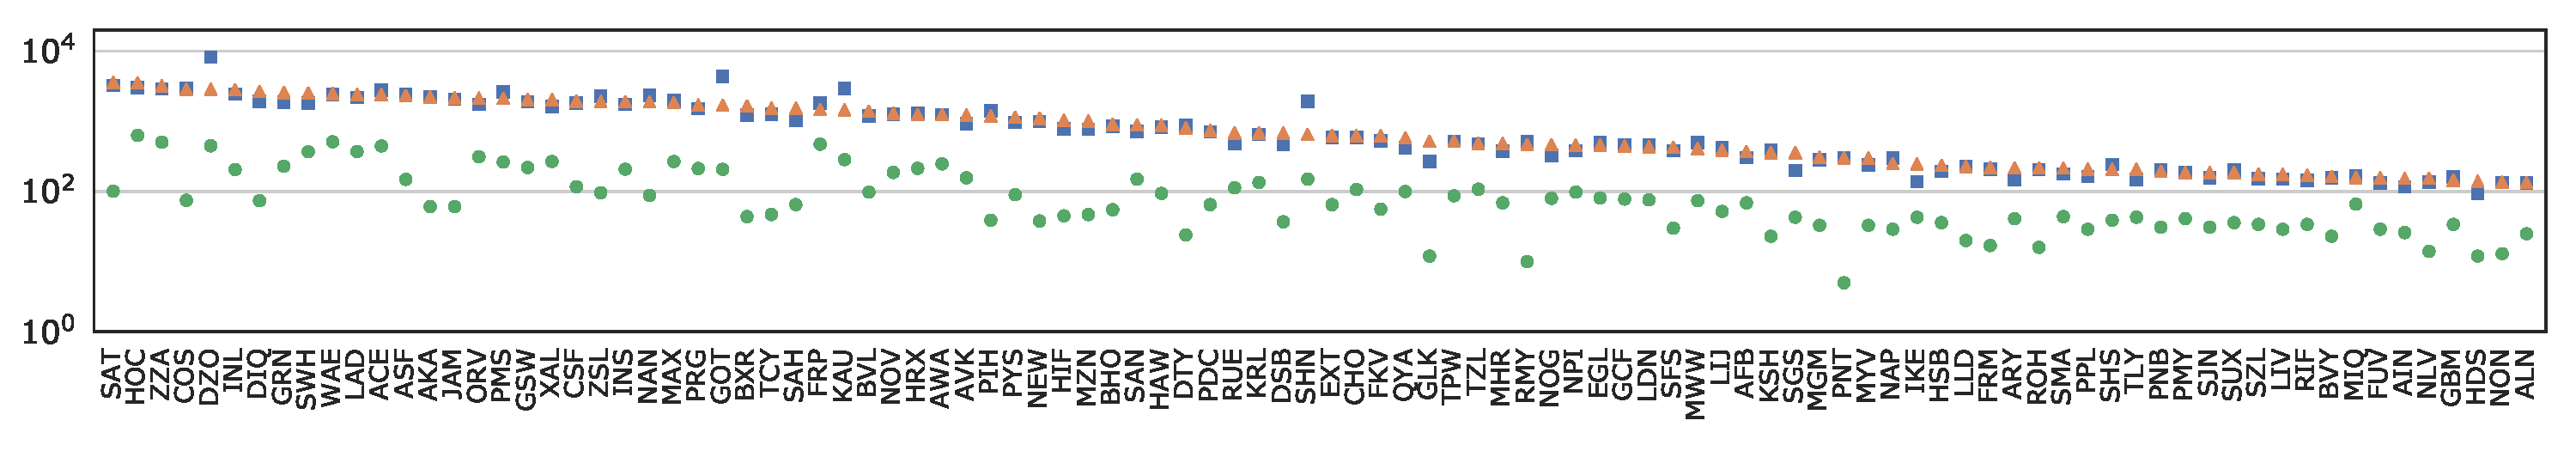
\includegraphics[height=0.14\vsize,trim={5mm 4mm 5mm 5mm},clip]{manyeng/lang-stats-401-500.pdf}     
    \caption{\centering Training data statistics for 500 languages, sorted as descending order of English token count,  obtained after de-duplication and filtering (see Section~\ref{sec:datasets}). The full name for these ISO 639-3 codes can be looked up using \mtdata, e.g. \texttt{mtdata-iso eng}. }
       \label{fig:train-data-stats}
\end{sidewaysfigure}
%\end{figure*}


\textbf{Cleaning:}
 We use \textsc{SacreMoses}\footnote{\url{https://github.com/isi-nlp/sacremoses} a fork of \url{https://github.com/alvations/sacremoses} with improvements to tokenization for many low resource languages.} to normalize Unicode punctuations and digits, followed by word tokenization. 
We remove records that are duplicates, have abnormal source-to-target length ratios, have many non-ASCII characters on the English side, have a URL, or which overlap exactly, either on the source or target side, with any sentences in held out sets.
As preprocessing is compute-intensive, we parallelize using Apache Spark.
The cleaning and tokenization results in a corpus of 474 million sentences and 9 billion tokens on the source and English sides each. The token and sentence count for each language are provided in Figure~\ref{fig:train-data-stats}.
Both the processed and raw datasets are available at \url{http://rtg.isi.edu/many-eng/data/v1/}.\footnote{A copy is at \url{https://opus.nlpl.eu/MT560.php}}

\subsection{Many-to-English Multilingual Model}
\label{sec:500eng-model}
We use \rtg\ to train Transformer NMT \cite{vaswani2017attention} with a few modifications.
Firstly, instead of a shared BPE vocabulary for both source and target, we use two separate BPE vocabularies. 
Since the source side has 500 languages but the target side has English only, we use a large source vocabulary and a relatively smaller target vocabulary.
A larger target vocabulary leads to higher time and memory complexity, whereas a large source vocabulary increases only the memory complexity but not the time complexity.
We train several models, ranging from the standard 6 layers, 512-dimensional Transformers to larger ones with more parameters. Since the dataset is massive, a larger model trained on big mini-batches yields the best results. Our best performing model is a 768 dimensional model with 12 attention heads, 9 encoder layers, 6 decoder layers, feed-forward dimension of 2048, dropout and label smoothing at 0.1, using $512,000$ and $64,000$ BPE types as source and target vocabularies, respectively. The decoder's input and output embeddings are shared.
Since some of the English sentences are replicated to align with many sentences from different languages (e.g. the Bible corpus), BPE merges are learned from the deduplicated sentences using \nlcodec.
Our best performing model is trained with an effective batch size of about 720,000 tokens per optimizer step. Such big batches are achieved by using mixed-precision distributed training on 8 NVIDIA A100 GPUs with gradient accumulation of 5 mini-batches, each having a maximum of 18,000 tokens. We use the Adam optimizer~\cite{kingma2015adam} with 8000 warm-up steps followed by a decaying learning rate, similar to \citet{vaswani2017attention}. 
We stop training after five days and six hours when a total of 200K updates are made by the optimizer; validation loss is still decreasing at this point. 
To assess the translation quality of our model, we report BLEU~\cite{papineni-etal-2002-bleu,post-2018-sacrebleu}\footnote{All our BLEU scores are obtained from \sacrebleu\ \texttt{BLEU+c.mixed+\#.1+s.exp+tok.13a+v.1.4.13}.} on a subset of languages for which known test sets are available, as given in Figure~\ref{fig:test-bleu}, along with a comparison to \citet{zhang-etal-2020-multiling-nmt}'s best model.\footnote{
%a multilingual 24-layered 512-dimensional Transformer model having Merged Attention, Language-aware Layer Normalization and Linear Transformation, and trained including random online backtranslation.
Scores are obtained from \url{https://github.com/bzhangGo/zero/tree/master/docs/multilingual_laln_lalt}; accessed: 2021/03/30}

\begin{figure*}[ht]
    \centering
    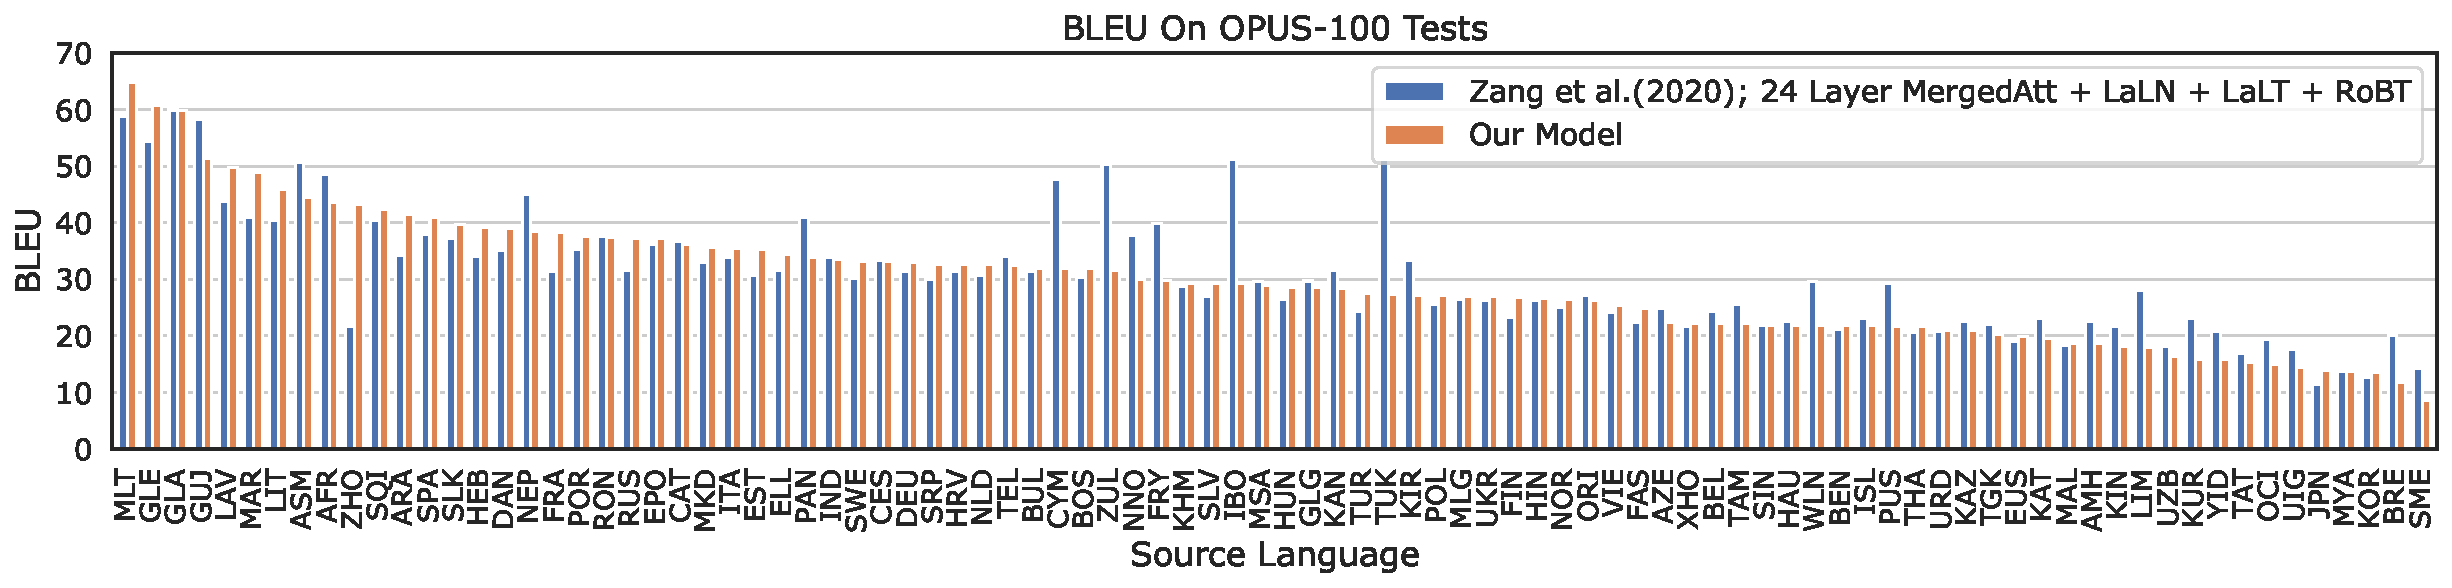
\includegraphics[width=\textwidth]{manyeng/BLEU-opus100.pdf}
    \caption[Caption for LOF]{Many-to-English BLEU on OPUS-100 tests~\cite{zhang-etal-2020-multiling-nmt}. 
    Despite having four times more languages on the source side, our model scores competitive BLEU on most languages with the strongest system of \citet{zhang-etal-2020-multiling-nmt}. The tests where our model scores lower BLEU have shorter source sentences (mean length of about three tokens).}
    \label{fig:test-bleu}
\end{figure*}
%All BLEU scores are mixed-cased and are obtained using the default settings of \sacrebleu.
% https://github.com/bzhangGo/zero/tree/master/docs/multilingual_laln_lalt

\begin{comment}
\begin{subfigure}[t]{0.68\textwidth}
        \centering
        \includegraphics[width=\linewidth]{manyeng/BLEU-nttalksv1.pdf}
        %\caption{Lorem ipsum}
    \end{subfigure}%
    ~ 
    \begin{subfigure}[t]{0.31\textwidth}
        \centering
        \includegraphics[width=\linewidth,trim={7mm 0mm 0mm 0mm},clip]{img/BLEU-wmt-etc.pdf}
        %\caption{Lorem ipsum}
    \end{subfigure}
     TED Talks~\cite{qi-etal-2018-pretrainemb}, WMT~\cite{barrault-etal-2019-findings}, UNv1~\cite{ziemski-etal-2016-unpc}, and Indian-6~\cite{post-etal-2012-constructing}.
\end{comment}



\section{Applications}
\label{sec:value}
The model we trained as a demonstration for our tools is useful on its own, as described in the following sections. 

\subsection{Readily Usable Translation Service}
\label{sec:value.off-shelf-mt}
Our pretrained NMT model is readily usable as a service capable of translating several hundred source languages to English.
By design, source language identification is not necessary.
Figure~\ref{fig:test-bleu} shows that the model scores more than 20 BLEU, which maybe be a useful quality for certain downstream applications involving web and social media content analysis.
Apache Tika \cite{mattmann2011tika}, a content detection and analysis toolkit capable of parsing thousands of file formats, has an option for translating any document into English using our multilingual NMT model.\footnote{\url{https://cwiki.apache.org/confluence/display/TIKA/NMT-RTG}} Our model has been packaged and published to DockerHub\footnote{\url{https://hub.docker.com/}}, which can be obtained by the following command:
\begin{minted}[
%frame=lines,
%framesep=2mm,
baselinestretch=1.1,
fontsize=\small,
%linenos
]{bash}
IMAGE=tgowda/rtg-model:500toEng-v1
docker run --rm -i -p 6060:6060 $IMAGE 
# For GPU support: --gpus '"device=0"' 
\end{minted}

The above command starts a docker image with HTTP server having a web interface, as can be seen in Figure~\ref{fig:rtg-webui}, and a REST API.
An example interaction with the REST API is as follows: 
\begin{figure}[ht]
    \centering
    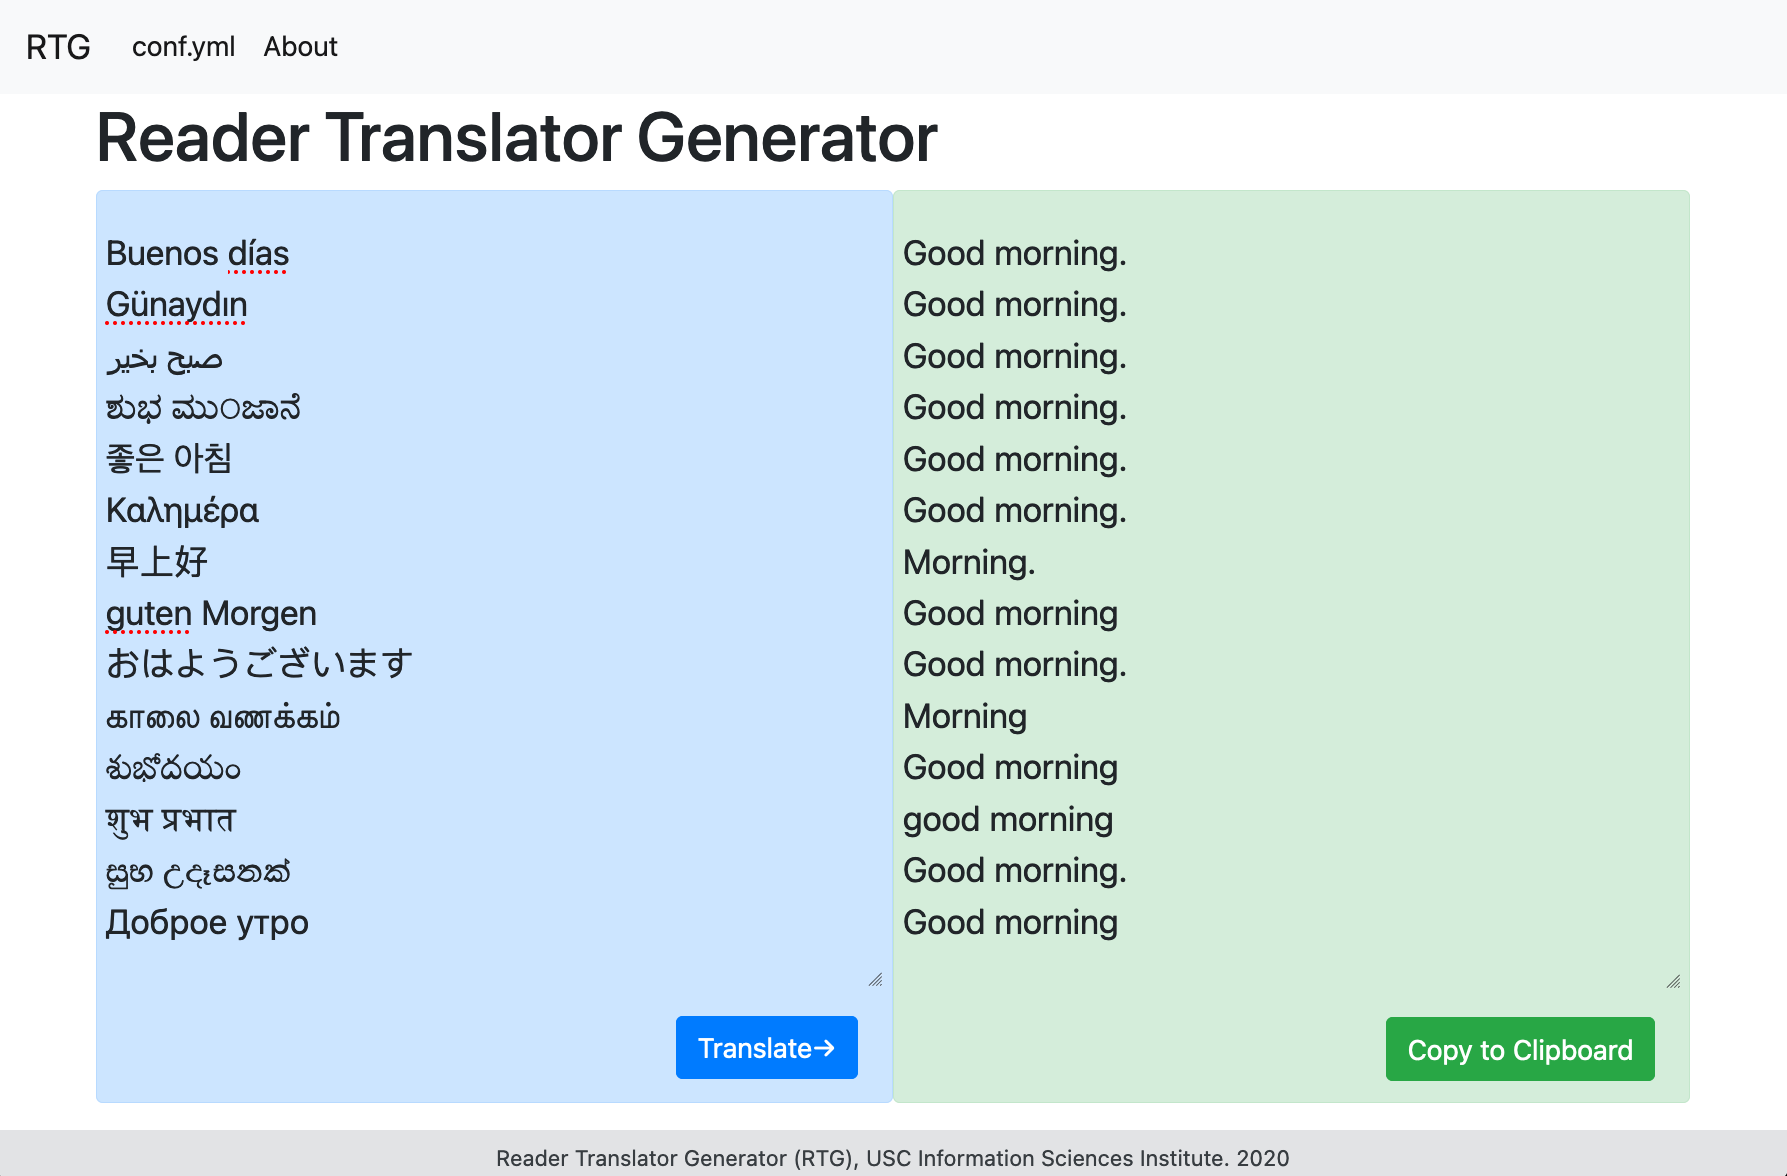
\includegraphics[width=0.6\linewidth,trim=20 60 100 15,clip]{manyeng/rtg-webui.png}
    \caption{RTG Web Interface}
    \label{fig:rtg-webui}
\end{figure}

\begin{minted}[baselinestretch=1.1, fontsize=\small]{bash}
curl --data "source=Comment allez-vous?"\
    --data "source=Bonne journée"\
    http://localhost:6060/translate
\end{minted}
\begin{minted}[baselinestretch=1.1, fontsize=\small]{json}
 {
  "source": [ "Comment allez-vous?",
        "Bonne journée" ],
  "translation": [ "How are you?", 
         "Have a nice day" ]
}
\end{minted}


\subsection{Parent Model for Low Resource MT}
\label{sec:value.transfer-learning}
%WMT 20 has two low resource languages: IU and KM http://statmt.org/wmt20/translation-task.html 
%Uyghur from Lorelei?  Pashto  from Material?
 Fine tuning is a useful transfer learning technique for improving the translation of low resource languages ~\cite{zoph-etal-2016-transfer,neubig-hu-2018-rapid,gheini2019universal}. 
For instance, consider Breton-English (BRE-ENG) and Northern Sami-English (SME-ENG), two of the low resource settings for which our model has relatively poor BLEU (see Figure~\ref{fig:test-bleu}). 
To show the utility of fine tuning with our model, we train a strong baseline Transformer model, one for each language, from scratch using OPUS-100 training data~\cite{zhang-etal-2020-multiling-nmt}, and finetune our multilingual model on the same dataset as the baselines. We shrink the parent model vocabulary and embeddings to the child model dataset, and train all models on NVIDIA P100 GPUs until convergence.\footnote{More info: \url{https://github.com/thammegowda/006-many-to-eng/tree/master/lowres-xfer}}
 Table~\ref{tab:transfer-lowres}, which shows BLEU on the OPUS-100 test set for the two low resource languages indicates that our multilingual NMT parent model can be further improved with finetuning on limited training data. The finetuned model is significantly better than baseline model.

\begin{table}[ht]
    \centering
    %\footnotesize
    \begin{tabular}{l  r r}
        Model     & BRE-ENG & SME-ENG \\ \hline\hline
        Baseline  & 12.7  &  10.7  \\
        Parent    & 11.8  &  8.6  \\
        \textit{Finetuned} & \textbf{22.8}  & \textbf{19.1}  \\ 
    \end{tabular}
    \caption{Finetuning our multilingual NMT on limited training data in low resource settings significantly improves translation quality, as quantified by BLEU.}
    \label{tab:transfer-lowres}
\end{table}

\subsection{Cross-lingual Contextual Embeddings}

The encoder of multilingual NMT model learns bi-directional contexualized embeddings that are cross-lingual across 500 languages.
We created a sequence classifier, and initialized the source embeddings matrix and all the encoder layers from our multilignual NMT. 
We finetuned the classifier on MultiNLI dataset having English training data, and evaluated on XNLI datasets on 15 languages. 
Such a setup is called as ``zero-shot'' or "cross-lingual transfer". 
Our model scores better performance than multilignual BERT, and it is competitive with XLM with translation modeling objective (XLM with MLM+TLM).



\section{Related work}

\subsection{Tools}
\textsc{SacreBleu}~\cite{post-2018-sacrebleu} simplifies MT evaluation.
\mtdata\ attempts to simplify training setup by automating training and validation dataset retrieval.
\textsc{OPUSTools}~\cite{aulamo-etal-2020-opustools} is a similar tool however, it interfaces with OPUS servers only.
Since the dataset index for \textsc{OPUSTools}~ is on a server, the addition of new datasets requires privileged access.
In contrast, \mtdata\ is a client side library, it can be easily forked and extended to include new datasets without needing special privileges. 

\textbf{\nlcodec:} 
\nlcodec\ is a Python library for vocabulary management. It overcomes the multithreading bottleneck in Python by using PySpark.
%It is made out of necessity to experiment with the core functionality of subword encoding schemes. 
\sentpiece~\cite{kudo-richardson-2018-sentencepiece} and \hftok~\cite{wolf-etal-2020-transformers} are the closest alternatives in terms of features, however, modification is relatively difficult for Python users as these libraries are implemented in C++ and Rust, respectively.
 %\nlcodec\ uses a tab-separated-values (TSV) format for model persistence, and \hftok\ uses JSON format; both of these are easily inspectable, however,
In addition, \sentpiece\ uses a binary format for model persistence in favor of efficiency, which takes away the inspectability of the model state. 
Retaining the ability to inspect models and modify core functionality is beneficial for further improving encoding schemes, e.g. subword regularization~\cite{kudo-2018-subwordreg}, BPE dropout~\cite{provilkov-etal-2020-bpedrop}, and optimal stop condition for subword merges~\cite{gowda-may-2020-finding}.
FastBPE is another efficient BPE tool written in C++.\footnote{\url{https://github.com/glample/fastBPE}}  
Subword-nmt~\cite{sennrich-etal-2016-bpe} is a Python implementation of BPE, and stores the model in an inspectable plain text format, however, it is not readily scalable to massive datasets such as the one used in this work.
None of these tools have an equivalent to \nldb's mechanism for efficiently storing and retrieving variable length sequences for distributed training.


\textbf{\rtg:}
Tensor2Tensor \cite{vaswani-etal-2018-tensor2tensor} originally offered the Transformer \cite{vaswani2017attention} implementation using Tensorflow~\cite{tensorflow2015-whitepaper}; 
our implementation uses Pytorch \cite{NEURIPS2019_Pytorch} following \textit{Annotated Transformer} \cite{rush-2018-annotated}.
OpenNMT currently offers separate implementations for both Pytorch and Tensorflow backends~\cite{klein-etal-2017-opennmt,klein-etal-2020-opennmt}.
As open-source toolkits evolve, many good features tend to propagate between them, leading to varying degrees of similarities. Some of the available NMT toolkits are:
Nematus~\cite{sennrich-etal-2017-nematus}, 
xNMT~\cite{neubig-etal-2018-xnmt}.
Marian NMT~\cite{junczys-dowmunt-etal-2018-marian-fast},
Joey NMT~\cite{kreutzer-etal-2019-joeynmt},
Fairseq~\cite{ott-etal-2019-fairseq}, and 
Sockey~\cite{hieber-etal-2020-sockeye}.
An exhaustive comparison of these NMT toolkits is beyond the scope of our current work.

\subsection{Multilingual NMT}
\citet{johnson-etal-2017-googleNMT} show that NMT models are capable of multilingual translation without any architectural changes, and observe that when languages with abundant data are mixed with low resource languages, the translation quality of low resource pairs are significantly improved. They use a private dataset of 12 language pairs; we use publicly available datasets for up to 500 languages. % with varying amounts of training data, aiming to improve translation of low resource languages. 
%\citet{neubig-hu-2018-rapid,gheini2019universal} show that pretrained multilingual NMT models are useful for adapting to low resource language pairs, which is one of the value of our pretrained model.
\citet{qi-etal-2018-pretrainemb} assemble a multi-parallel dataset for 58 languages from TEDTalks domains, which are included in our dataset. 
%\citet{aharoni-etal-2019-massively} conduct a study on massively multilingual NMT, use a dataset having 102 languages which is not publicly available.
\citet{zhang-etal-2020-multiling-nmt} curate OPUS-100, a multilingual dataset of 100 languages sampled from OPUS, including test sets; which are used in this work.
\citet{tiedemann-2020-tatoeba} have established a benchmark task for 500 languages  including single directional baseline models.
\citet{wang-etal-2020-balancing} examine the language-wise imbalance problem in multilingual datasets and propose a method to address the imbalance using a scoring function, which we plan to explore in the future.



\section{Conclusion}

We have introduced our tools: \mtdata\ for downloading datasets, \nlcodec\ for processing, storing and retrieving large scale training data, and \rtg\ for training NMT models.
Using these tools, we have collected a massive dataset and trained a multilingual model for many-to-English translation.
We have demonstrated that our model can be used independently as a translation service, and also showed its use as a parent model for improving low resource language translation. 
All the described tools, used datasets, and trained models are made available to the public for free. 

\section*{Acknowledgments}
The authors would like to thank Lukas Ferrer, Luke Miles, and Mozhdeh Gheini for their contributions to some of the tools used in this work, and thank Jörg Tiedemann for hosting our prepared dataset at OPUS (\url{https://opus.nlpl.eu/MT560.php}). 
The authors acknowledge the Center for Advanced Research Computing (CARC) at the University of Southern California for providing computing resources that have contributed to the research results reported within this publication. URL: \url{https://carc.usc.edu}. 
The authors acknowledge the Texas Advanced Computing Center (TACC) at The University of Texas at Austin for providing HPC resources that have contributed to the research results reported within this paper. URL: \url{http://www.tacc.utexas.edu}. This research is based upon work supported by the Office of the Director of National Intelligence (ODNI), Intelligence Advanced Research Projects Activity (IARPA), via AFRL Contract FA8650-17-C-9116.  The views and conclusions contained herein are those of the authors and should not be interpreted as necessarily representing the official policies or endorsements, either expressed or implied, of the ODNI, IARPA, or the U.S. Government. The U.S. Government is authorized to reproduce and distribute reprints for Governmental purposes notwithstanding any copyright annotation thereon.





\section*{Ethical Consideration}

\textit{Failure Modes:} \mtdata\ will fail to operate, unless patched, when hosting services change their URLs or formats over time.
On certain scenarios when a dataset has been previously accessed and retained in local cache, \mtdata\ continues to operate with a copy of previous version and ignores server side updates.
We have done our best effort in normalizing languages to ISO 639-3 standard; our current version does not accommodate country and script variations of languages; e.g. UK English and US English are both mapped to \textit{eng}. 
Our multilingual NMT model is trained to translate a full sentence at a time without considering source language information; translation of short phrases without a proper context might result in a poor quality translation. 

\textit{Diversity and Fairness:}
We cover all languages on the source side for which publicly available dataset exists, which happens to be about 500 source languages. 
Our model translates to English only, hence only English speakers are benefited from this work. 


\textit{Climate Impact:}
\mtdata\ reduces network transfers to the minimal by maintaining a local cache to avoid repetitive downloads.
In addition to the raw datasets, preprocessed data is also available to avoid repetitive computation.
Our Multilingual NMT has higher energy cost than a typical single directional NMT model due to higher number of parameters, however, since our single model translates hundreds of languages, the energy requirement is significantly lower than the total consumption of all independent models. 
Our trained models with all the weights are also made available for download.


\textit{Dataset Ownership:}
\mtdata\ is a client side library that does not have the ownership of datasets in its index.
Addition, removal, or modification in its index is to be submitted by creating an issue at \url{https://github.com/thammegowda/mtdata/issues}. 
We ask the dataset users to review the dataset license, and acknowledge its original creators by citing their work, whose \BibTeX\ entries may be accessed using:\\ \texttt{\footnotesize mtdata list -n <NAME> -l <L1-L2> --full} \\
The prepared dataset that we have made available for download includes \texttt{citations.bib} that acknowledges all the original creators of datasets.
We do not vouch for quality and fairness of all the datasets.

%-----------------------------------------------------------------------------
%	BIBLIOGRAPHY / REFERENCES
%-----------------------------------------------------------------------------
\begin{singlespace}
\bibliography{anthology}
%\bibliographystyle{acl_natbib}
\bibliographystyle{acl_natbib}
\end{singlespace}


%-----------------------------------------------------------------------------
%	APPENDICES
%-----------------------------------------------------------------------------
\appendix

\chapter{Placeholder Appendix}

\section{Section Placeholder}
Some place holder text



%\backmatter
\end{document}
